


 
\documentclass[10pt]{article}
\usepackage[utf8]{inputenc}
\usepackage{mathtools,amsmath,amssymb}
\usepackage{graphicx}
\usepackage{lmodern}
\usepackage[T1]{fontenc}
%\usepackage{microtype}
\usepackage[pagebackref=false]{hyperref}
\usepackage{bbm}
\usepackage{bm}
\usepackage{appendix}
\usepackage{comment}
\usepackage{mathtools}
\usepackage{array}
\numberwithin{equation}{section}
\numberwithin{equation}{subsection}





%\usepackage[textsize=tiny]{todonotes}
 
% \usepackage[notref,notcite]{showkeys}
\usepackage{xspace}
%\usepackage{bibentry}
%\usepackage{easybmat}

\usepackage{graphicx}

\usepackage{subcaption} 

%\usepackage[numbers,sort&compress]{natbib}
%\usepackage{hypernat}
 
\usepackage{tikz}
\usetikzlibrary{decorations.pathreplacing}
% MACROS
% % 
% \newcommand{\cristian}[1]{{\bf (* {\color{ForestGreen}V:{} \small #1}*)}}
% \newcommand{\jorge}[1]{{\bf (* {\color{BlueViolet}G:{} \small #1}*)}}
% \newcommand{\rouven}[1]{{ (* {\color{red}{} \small #1}*)}}
\newtheorem{definition}{Definition}
\newtheorem{theorem}{Theorem}
\newtheorem{proposition}{Proposition}
\newtheorem{lemma}{Lemma}
\newtheorem{corollary}{Corollary}
\newtheorem{remark}{Remark}
\frenchspacing

\newcommand{\changelocaltocdepth}[1]{%
  \addtocontents{toc}{\protect\setcounter{tocdepth}{#1}}%
  \setcounter{tocdepth}{#1}%
}
\newcommand{\id}{I}
\newcommand{\Xt}{\widetilde{X}}
\newcommand{\co}{\;,}
\newcommand{\dt}{\;.}


\newcommand{\len}{L}
\newcommand{\spe}{N}


\newcommand{\com}[1]{{ (* {\color{red}\small #1}*)}}


\setcounter{tocdepth}{2}

\usepackage[margin=2.5cm]{geometry} 

%%%%%  oscillators
\newcommand{\osc}[1]{\mathbf{#1}}
\newcommand{\oscgreea}[1]{\boldsymbol{#1}}
\newcommand{\dagg}[1]{\bar{#1}}
\newcommand{\ep}{\epsilon}
\newcommand{\ob}{\osc{b}}
\newcommand{\oc}{\osc{c}}
\newcommand{\od}{\osc{d}}
\newcommand{\oab}{\dagg{\osc{a}}}
\newcommand{\obb}{\dagg{\osc{b}}}
\newcommand{\ocb}{\dagg{\osc{c}}}
\newcommand{\odb}{\dagg{\osc{d}}}
\newcommand{\ox}{\oscgreek{\xi}}
\newcommand{\oxb}{\dagg{\oscgreek{\xi}}}
\newcommand{\och}{\oscgreek{\chi}}
\newcommand{\ochb}{\dagg{\oscgreek{\chi}}}
\newcommand{\NN}{\mathbf{N}}
\newcommand{\ccc}{\mathbf{C}}
\newcommand{\qop}{Q}
\newcommand{\sop}{Y}
\newcommand{\q}{\mathbf{\epsilon}}
\newcommand{\ID}{I}
\newcommand{\per}{P}

\newcommand{\EE}{\mathrm{E}}

\newmuskip\pFqmuskip

\newcommand*\pFq[6][8]{%
  \begingroup % only local assignments
  \pFqmuskip=#1mu\relax
  \mathchardef\normalcomma=\mathcode`,
  % make the comma math active
  \mathcode`\,=\string"8000
  % and define it to be \pFqcomma
  \begingroup\lccode`\~=`\,
  \lowercase{\endgroup\let~}\pFqcomma
  % typeset the formula
  {}_{#2}\phi_{#3}{\left[\genfrac..{0pt}{}{#4}{#5};#6\right]}%
  \endgroup
}
\newcommand{\pFqcomma}{{\normalcomma}\mskip\pFqmuskip}


\DeclareMathOperator{\tr}{tr}
\DeclareMathOperator{\Li}{Li}
\DeclareMathOperator{\diag}{diag}


\newcommand{\KL}{\mathcal{K}}
\newcommand{\KR}{\hat{\mathcal{K}}}
\newcommand{\oa}{\mathbf{a}}
\newcommand{\dd}{\mathcal{D}_{u(x)}}
\newcommand{\oad}{\mathbf{a}^{+}}

\newcommand{\phil}{\beta_-}
\newcommand{\phir}{\beta_+}
\newcommand{\ma}{n}

\newcommand{\oaq}{\mathbf{a}_\q}

\newcommand{\oadq}{\mathbf{\bar{a}}_\q}

\newcommand{\N}{\mathbf{N}}
\newcommand{\twoj}{\nu}
\allowdisplaybreaks



\begin{document} 
 
\begingroup
% \centering
\begin{center}
 \begingroup\LARGE
%\bf Multispecies stirring process: duality and exact solution
\bf Multispecies stirring process \\
 with open boundaries
\par\endgroup
 \vspace{3.5em}
 \begingroup\large \bf
% {Rouven Frassek}
 \par\endgroup
\vspace{2em}

\begingroup\sffamily 
%  
% Università degli Studi di Modena e Reggio Emilia
%University of Modena and Reggio Emilia, 
%\\Department of Physics, Informatics and Mathematics,\\
%Via G. Campi 213/b, 41125 Modena, Italy\\ 
\par\endgroup
\vspace{2em}

 Version: \today
\end{center}
%  

\thispagestyle{empty}

\begin{abstract}
\noindent
...
\end{abstract}

%\vfill 

\tableofcontents

% \newpage

\section{Introduction} 
In the past years duality has been developed to study stochastic processes, especially in the boundary driven case, i.e. when the system is put in contact with boundaries that generate a non-equilibrium current. The literature is huge. We can address , for instance, to \cite{giardina2009duality,carinci2013duality,frassek2020duality}. One application of duality is the attempt to characterize the non equilibrium steady state of boundary driven process via the so called absorption probabilities. Indeed, there are many cases where the dual process has absorbing boundaries. This means that the the chain is eventually empty in the long time scale. Moreover, there are cases in which the steady state of a stochastic process can be computed explicitly, thanks to the integrability property of the system (quantum inverse scattering method, matrix product ansatz). In this direction, some examples can be found in \cite{derrida1993exact,frassek2019non,frassek2020eigenstates}. In the past, the focus has been on processes where one can distinguish, in each site of a certain graph, a (or many) particles or an empty state. However, this particles are indistinguishable, in the sense that you can pile up in a site just one type of particles. Some natural questions arise: what happens if we imagine to assign different colours to the particles? Is the duality property still holding? How far can we push our analysis for the characterization of the non equilibrium steady state?\\
The way one can define a multi-type (or multi-species) interacting particle system is not unique. In the literature there are many. Two of them are the following. On one hand, the \textit{multi-layer models}, in which the process is constructed on a many layer graph where each graph correspond to a type and perform a kind of dynamic (independent jump, exclusion/inclusion walkers) and the layers communicate each other with some "switching probabilities". The state space of the Markov process is the Cartesian product of the state spaces of each layer, i.e. of the two species. For example see \cite{floreani2022switching,redig2022ergodic,redig2023equilibrium}. On the other hand, the \textit{single layer models}. Here, there is just one layer, where particles of each type can pile up, in a way that the exclusion dynamic concerns many species together. In other words, now the species can interact "directly", not just by switching layer. Here the state space contains all the species and it is not product anymore. Some examples of such a dynamic can be found in \cite{casini2022uphill,vanicat2017exact,zhou2021orthogonal,casini2023density}. \\
In this work we concentrate our effort in this last "single layer" case with a repulsive process, i.e. a dynamic in which a maximum amount of particles can be present in each site at each time. We will call this amount, the "maximal occupancy" and it will indicated with $\twoj$ where $\twoj\in\mathbb{N}$. Particle of any species can exchange their position in the graph, under this exclusion constraint. The system will be put out of equilibrium and some absorbing duality result are investigated. Moreover, we will use this duality, to study the out of equilibrium steady state. In particular, in case of $\twoj=1$ we retrieve the model studied in \cite{vanicat2017exact}. 
{\color{red}
The case of $\twoj=1$ distinguishes itself from other values of $\twoj$ as in this case the model can be mapped to an integrable higher rank $gl(N)$ Heisenberg XXX spin chain with open (non-diagonal) boundaries. Furthermore the matrix product ansatz \cite{derrida1993exact}  is applicable, see \cite{Crampe:2014aoa,vanicat2017exact}.
}
We will exploit the duality and the underlying symmetries of the model, to write explicitly all the correlations of this \textit{hard-core exclusion} case. The main tool that we will use is the Lie algebraic description of the process, that allows to find the duality as a proper symmetry of the generator. \\
 For a complete review of the quantum inverse scattering method see \cite{Sklyanin:1988yz} and \cite{faddeev1996algebraic}. For application of the QISM to interacting particle systems we refer to \cite{frassek2020eigenstates,frassek2019non,frassek2022exact,vanicat2017exact}. \\
 A new technique to compute absorption probabilities has been proposed in \cite{floreani2023non}.
\paragraph{Organization of the paper}
%
%
%
%
\section{The stirring process with open boundaries}
\subsection{Informal description of the process}
The process studied in this paper is the {\em multi-species stirring process}
with open boundaries. 
In words, the dynamics is described as follows. Each site
of a connected graph can host up to $\nu\in \mathbb{N}$ particles.
The particles have a {\em type} (sometimes called {\em species} or {\em color})
which can take $N$ values.
Then, the dynamics has two parts: on each edge of the graph, 
any two types are swapped at rate $1$; additionally, on each site $x$, 
a particles of a given type (if present) is replaced with a
particle of type $a$ at rate $\alpha_a^x >0$.
The swap dynamics taking place on the edges is of Kawasaki-type 
with $N$ conservation laws
(the total number of particles of each type). 
The site-dynamics is instead of Glauber-type. 
In the long-time limit, a so-called non-equilibrium
steady state sets in.


\noindent
\begin{remark}
\label{hole}
In the following we will often consider type $N$ as a distinguished type
(called `holes'), whose number at each site is fixed by the numbers of particles 
of the remaining $N-1$ types. It is interesting to observe that, in case we stop distinguishing the types of the ``true'' particles of types 
(those of types $\{1,\ldots,N-1\}$), we retrieve the 
boundary-driven version of the partial symmetric exclusion process \cite{schutzSandow,carinci2013duality}.
The choice of type $N$ for the distinguished type is arbitrary and does not affect
the results. In particular, we shall see in Section \ref{sectionDuality} about duality, that
the dual process eventually has only particles of type $N$ on the graph.
Interpreting type $N$ as an hole, one can then say that the dual process voids the graph.  
\end{remark}






\subsection{The process generator}\label{subsectionGeneratorStr}
We now give the mathematical description of the multi-species stirring process.
We consider a connected graph $G=(V,\mathcal{E})$ with vertex set $V$ and edge set $\mathcal{E}$.
At each vertex site $x\in V$, we describe the occupation with an $N-$dimensional vector $n^{x}=(n_{1}^{x},\ldots,n_{N}^{x})$ in which the value of the $a$-th component $n_{a}^{x}$ denotes the number of particles of species $a\in \{1,\ldots,N\}$. On each vertex we allow a total  maximal occupancy $\nu\in \mathbb{N}$. Then, the configuration space of the process on the graph $G$ is 
\begin{equation}\label{stateSpace}
    \Omega:=\bigotimes_{x\in V} \Omega_{x}
\end{equation}
where
\begin{equation}
\Omega_{x}:=\left\{n^x=(n_{1}^{x},\ldots,n_{N}^{x})\in\mathbb{N}_0^{N}\;:\; \sum_{a=1}^{N}n_{a}^{x}=\twoj\right\}\,.
\end{equation}
We denote a particle configuration on the graph as $\bm{n}\in \Omega$, where $\bm{n}=(n_{a}^{x})_{x\in V,\,a\in\{1,\ldots,N\}}$.
The infinitesimal generator of the process reads
\begin{equation}\label{Generator}
    \mathcal{L}=\sum_{(x,y)\in \mathcal{E}}\omega_{x,y}\mathcal{L}_{x,y}+\sum_{x\in V}\Gamma_{x}\mathcal{L}_{x}
\end{equation}
where  $ \omega_{x,y}\geq 0$ are so-called conductances and $\Gamma_{x}\geq 0$ are the couplings to reservoirs. 
The generator $\mathcal{L}_{x,y}$ is called the \textit{edge generator}, while $\mathcal{L}_{x}$ is called the \textit{site generator}. These linear operators act on functions $f:\Omega\to \mathbb{R}$ as follows
\begin{equation}\label{edgeGenerator}
\mathcal{L}_{x,y}f(\bm{n})=\sum_{a,b=1}^{N}n_{a}^{x}n_{b}^{y}\left[f(\bm{n}-\bm{\delta}^{x}_{a}+\bm{\delta}_{b}^{x}+\bm{\delta}_{a}^{y}-\bm{\delta}_{b}^{y})-f(\bm{n})\right]\co
\end{equation}
\begin{equation}\label{siteGenerator}
    \mathcal{L}_{x}f(\bm{n})=\sum_{a,b=1}^{N}\alpha_{a}^{x}n_{b}^{x}\left[f(\bm{n}+\bm{\delta}_{a}^{x}-\bm{\delta}_{b}^{x})-f(\bm{n})\right]\co
\end{equation}
where 
\begin{equation}
(\bm{\delta}_{a}^{x})^{y}_{b}=\begin{cases}
1\qquad &\text{if}\quad y=x,\;b=a\;,\\
0\qquad &\text{otherwise}\dt
\end{cases}
\end{equation}
Thus the dynamics consists in an exchange of particles between connected vertices at Poissonian times. 
This means that on the edge $(x,y)\in \mathcal{E}$  a particle of type $a$ at site $x$ is exchanged with a particle of type $b$ at site $y$ at rate $\omega_{x,y}n_{a}^{x}n_{b}^{y}$. 
Moreover, each vertex  exchanges particles with the external environment (reservoirs). 
Namely, on each site $x\in V$  a particle of type $b$ is replaced with a particle of type $a$ at rate $\Gamma_{x}\alpha_{a}^{x}n_{b}^{x}$. 
%
%For the sake of notation we denote $|\alpha^{x}|=\sum_{a=1}^{N}\alpha_{a}^{x}$. 
%See Figure \ref{fig:1} and  Figure \ref{fig:2} for a visualisation of the dynamics. 
%\begin{figure}[h]
%    \centering
%    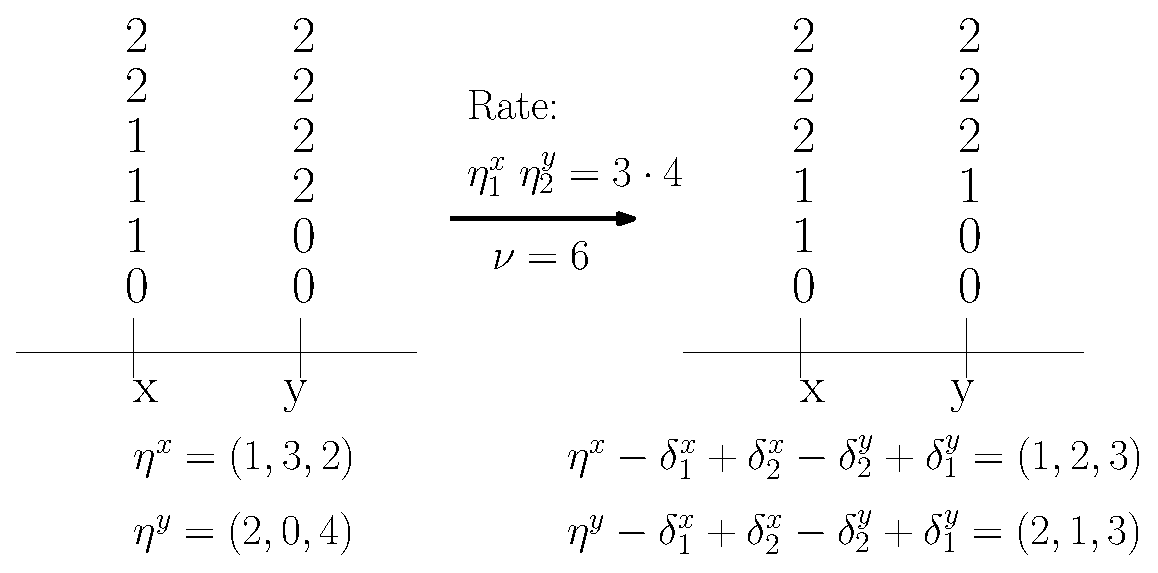
\includegraphics[scale=0.45]{BulkStirring.eps}
%    \caption{The edge dynamics. Maximal occupation is $\nu=6$. A particle of type $2$ is removed in $x$ and placed in $y$. A particle of type $3$ is removed in $y$ and placed in $x$. This transition occurs at rate $n_{2}^{x}n_{3}^{y}=2\cdot 3$.}
%    \label{fig:1}
%\end{figure}
%\begin{figure}[h]
%    \centering
%    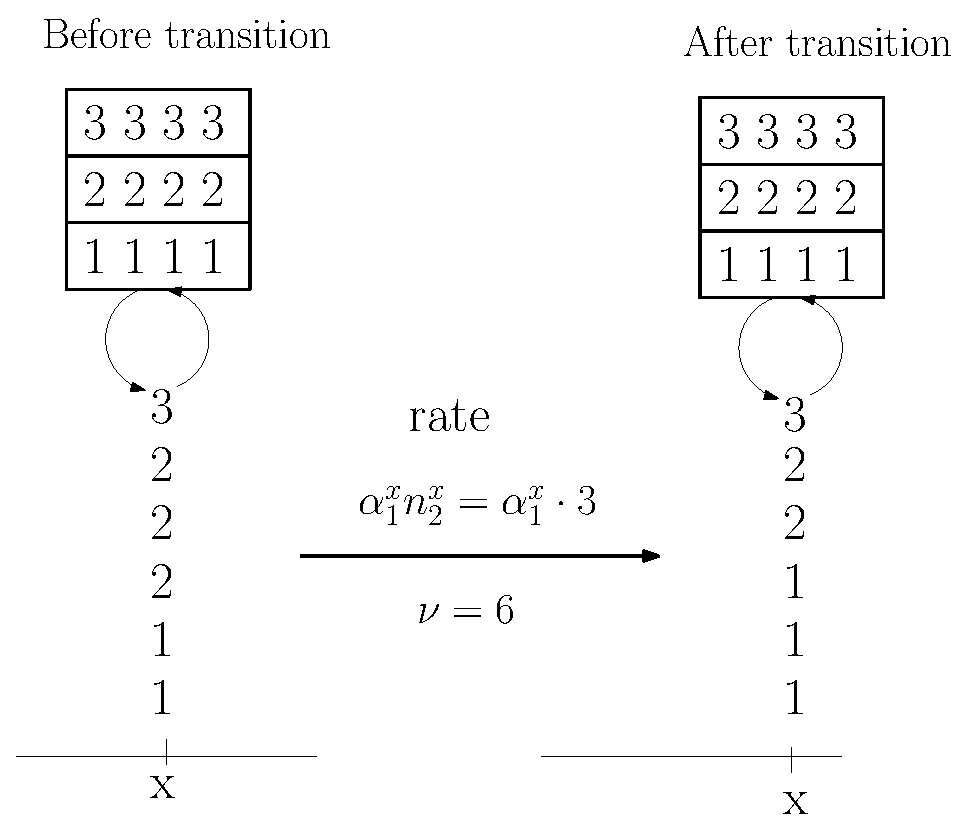
\includegraphics[scale=0.4]{BoundaryStirring.eps}
%    \caption{The site dynamics. Here the maxiaml occupation is $\nu=6$. The reservoir, represented by a square "box" containing all types of particles, remove a type $2$ from site $x$ and replace it with a type $3$. This transition occurs at rate $\alpha_{3}^{x}n_{2}^{x}$.}
%    \label{fig:2}
%\end{figure}
\subsection{Reversible measures in the equilibrium set-up}
For a particular choice of the reservoir parameters one has an $N$-parameter family of reversible measures. More precisely
when the parameters are the same on each site, i.e.
\begin{equation}\label{reversibilityCondition}
\alpha_{a}^{x}=\alpha_{a}\qquad \forall x\in V\,,
\end{equation}
then the process described by the generator \eqref{Generator} is reversible with respect to the 
homogeneous product measure 
\begin{equation}
\label{reversibleMeasure}
\mu_{\text{rev}}=\bigotimes_{x\in V}\mu_{\text{rev}}^{x}
\end{equation}
with marginals $\mu_{\text{rev}}^{x}$ given by 
\begin{equation}
 \mu^{x}_{\text{rev}}\sim \text{Multinomial}\left(\twoj,\rho_{1},\ldots,\rho_{N}\right)\,.
\end{equation}
Here
 $$
\rho_{a}=\frac{\alpha_{a}}{|\alpha|}\co
$$
is the density of specie $a$ and we used the notation $|\alpha|=\sum_{a=1}^{N}\alpha_{a}$. Explicitly, 
\begin{equation}
\mu_{\text{rev}}^{x}(n^{x})=\frac{\nu!}{\prod_{a=1}^{N}n_{a}^{x}!}\prod_{a=1}^{N}\rho_{a}^{n_{a}^{x}}\,.
\end{equation}
This can be proved  by checking that detailed balance is satisfied. 
If condition \eqref{reversibilityCondition} is not met, then reversibility is lost: each reservoir at site $x$ wants to fix its own set of densities $\rho^{x}=(\rho_{1}^{x},\ldots,\rho_{N}^{x})$ with
\begin{equation}
\label{rhox}
\rho_{a}^x=\frac{\alpha_{a}}{|\alpha^x|}
\end{equation}
and  $|\alpha^x|=\sum_{a=1}^{N}\alpha_{a}$. 
Currents will arise when at least two reservoirs have different densities. 

\subsection{Lie algebraic description of the process}

In this paper we will often use the fact that the Markov generator of the multispecies stirring process can be described in terms a Lie algebra of rank $N$.
In this section we provide details about this.

Consider the Lie algebra $gl(N)$ with generators denoted by $\EE_{ab}$ with $a,b\in \{1,\ldots,N\}$ and commutation relations
\begin{equation}\label{eq:comgl}
\left[\EE_{ab},\EE_{cd}\right]=\EE_{ad}\delta_{cb}-\EE_{cb}\delta_{ad}\qquad \forall a,b\in \{1,\ldots,N\}\,.
\end{equation}
The finite-dimensional representations are labelled by partitions $\lambda=(\lambda_1,\lambda_2,\ldots,\lambda_N)$ of $\nu$ with  $\lambda_i\geq \lambda_{i+1}$,  $\lambda_i\in \mathbb{N}$ and $\sum_{i=1}^N \lambda_i = \nu\in\mathbb{N}$.  
We are interested in the {\em symmetric} finite-dimensional representations with 
\begin{equation}\label{eq:dynkin}
    \lambda=(\twoj,0,\ldots,0) \;.
    %\qquad\text{where}\qquad \twoj\in\mathbb{N}\,.
\end{equation} 
The dimension $M_\twoj$ of this symmetric representations is given by the combination of $N$ objects in $\twoj$ positions with repetition, namely
\begin{equation}
	M_\twoj= \frac{(N+\twoj-1)!}{\twoj  !(N-1)!}\dt
\end{equation} 
The generators of the symmetric representations will be denoted by $E_{ab}$.
A basis of the vector space $\mathbb{C}^{M_\twoj}$ are the column vectors denoted by
\begin{equation}
  |n\rangle=  |n_{1},\ldots,n_{N}\rangle,\quad \text{with}\quad n_{i}\in\mathbb{N}_{0}\quad \text{sucht that}\quad \sum_{i=1}^{N}n_{i}=\nu\,.
\end{equation}
%where $\sum_{a=1}^{N}n_{i}=\nu$. 
The basis vectors satisfy the orthogonality relation
\begin{equation}\label{ortho}
   \langle m|n \rangle =\langle m_{1},\ldots,m_{N}|n_{1},\ldots,n_{N}\rangle=\prod_{a=1}^{N}\delta_{m_{a},n_{a}}\co
\end{equation}
where  $ \langle m_{1},\ldots,m_{N}|$ is the row vectors obtained by transposing $|m\rangle=|m_{1},\ldots,m_{N}\rangle$ and $\delta_{m_{a},n_{a}}$ is the Kronecker delta. 

The explicit action of the algebra generators on the basis  vectors $|n\rangle$ is the following:
\begin{equation}\label{actionE}
	\begin{cases}
		E_{ab}|n_{1},\ldots,n_{a},\ldots,n_{b},\ldots,n_{N}\rangle =n_{b}|n_{1},\ldots,n_{a}+1,\ldots,n_{b}-1,\ldots,n_{N}\rangle\qquad\qquad a\neq b\\[0.1cm]
		E_{aa}|n_{1},\ldots,n_{a},\ldots,n_{N}\rangle = n_{a} |n_{1},\ldots,n_{a},\ldots,n_{N}\rangle\dt
	\end{cases}
\end{equation}  
The matrices defined in this way satisfy the commutation relations \eqref{eq:comgl} and yield Dynkin weight \eqref{eq:dynkin}. \\
%{\color{red} Is this remark relevant for us?}
%\newline 
%\textbf{Remark}: it is possible to define these matrices in terms of creation and annihilation operators: see Appendix \ref{appA}.
\\ \\
%\textbf{Remark}: The symmetric representations $\lambda=(\twoj,0,\ldots,0)$ are dual to the representations $\lambda=(\twoj,\ldots,\twoj,0)$ that can be obtained via 
%\begin{equation}
%   \bar E_{ab}=\nu\delta_{ab}-E_{N-b+1,N-a+1}\dt
%\end{equation}
%{\color{red} This needs to be checked and give alternative form of Hamiltonian?}\\
The process with generator \eqref{Generator} can be described in terms of $gl(N)$ Lie algebra generators. The state space \eqref{stateSpace} is given by the $|V|$-fold tensor product of the vector space with basis elements $|n^x\rangle$ at a given site. Namely,
a vector $|{\bf n}\rangle \in \Omega$ can be written as
%We now define the equivalent of \eqref{stateSpace} in the vector notation
% \begin{equation}
%	\Omega':=\left\{|n\rangle=|n_{1},\ldots,n_{N}\rangle \;:\;n\in\mathbb{N}_0^N,\;\;|n|=\twoj\right\}^{\otimes|V|}
%	\end{equation}
%where we denote 
\begin{equation}
|{\bf n}\rangle=\left(\,\bigotimes_{x\in V}	|n_{1}^{x},\ldots,n_{N}^{x}\rangle\right)
\end{equation}
%{\color{blue}
%	\begin{equation*}
%		|{\bf n}\rangle=\left(\,\bigotimes_{x\in V}	|n_{1},\ldots,n_{N}\rangle_{x}\right)
%	\end{equation*}}
%where we require that $n_{a}^{x}\in \mathbb{N}_{0}$ and $\forall x\in V$ we have 
with $\sum_{a=1}^{N}n_{a}^{x}=\nu$ for any $x\in V$. Sometimes it will bw convenient to write $|n^{x}\rangle$ to denote, for a fixed $x\in V$, the vector $|n_{1}^{x},\ldots,n_{N}^{x}\rangle$.
The following orthogonality relation is a consequence of the single site relation \eqref{ortho}
\begin{equation}
    \langle {\bf n}|{\bf m}\rangle =\prod_{x\in V}\prod_{a=1}^N\delta_{n^x_a,m^{x}_a}\,.
\end{equation}
We introduce the Hamiltonian operator
\begin{equation}\label{OriginalHamiltonian}
	\begin{split}
		H=\sum_{(x,y)\in \mathcal{E}}\omega_{x,y}\mathcal{H}_{x,y}+\sum_{x\in V}\Gamma_{x}H_{x}
	\end{split}
\end{equation}
where the edge Hamiltonian that describes the interaction between two connected sites is
\begin{equation}\label{edgeHamiltonian}
\mathcal{H}_{x,y}=\sum_{a,b=1}^{N}\Big(E_{ab}^{x} E_{b a}^{y}-E_{bb}^{x} E_{aa}^{y}\Big)
 \end{equation}
  and where the site Hamiltonian is
 \begin{equation}\label{siteHamiltonian}
H_{x}=\sum_{a,b=1}^{N}\alpha_{a}^{x}\left(E_{ab}^{x}-E_{bb}^{x}\right)
\end{equation}
Here $E_{ab}^{x}$ is a copy of $E_{ab}$ defined in \eqref{actionE} acting on site $x$ (and
acting trivially as the identity on the other sites). 
Following  \cite{belitsky2015self}, the Hamiltonian and the Markov generator are linked by
\begin{equation}\label{Hamiltonian-Generator}
H=\mathcal{L}^{T}\dt
\end{equation}
The action of the generator can also be expressed as 
\begin{equation}
    \mathcal{L}f( {\bf n})=\langle f|H| {\bf n}\rangle
\end{equation}
where 
\begin{equation}
    \langle f|=\sum_{ {{\bf m}\in \Omega}}f( {\bf m})\langle  {\bf m}|
\end{equation}

We can write the edge Hamiltonian \eqref{edgeHamiltonian} as a function of the coproduct of the quadratic Casimir of $gl(N)$
\begin{equation}\label{secondCasimir}
    C=\sum_{a,b=1}^{N}E_{ab}E_{ba}
\end{equation}
that acts diagonally as $C|\bm{n}\rangle=\twoj(\twoj+N)|\bm{n}\rangle$ and belogs to the center of $gl(N)$ (i.e. it commutes with all the algebra elements).  
More precisely,  considering the standard coproduct 
\begin{equation}
\begin{split}
\Delta:gl(N)&\to gl(N)\otimes gl(N)\\
E_{ab}&\mapsto E_{ab}\otimes \mathbbm{1}+\mathbbm{1}\otimes E_{ab}
\end{split}
\end{equation}
we have 
\begin{equation}
\Delta(C)=\sum_{a,b=1}^{N}\Delta(E_{ab})\Delta(E_{ba})=2\sum_{a,b=1}^{N}E_{ab}\otimes E_{ba}+C\otimes \mathbbm{1}+\mathbbm{1}\otimes C\,.
\end{equation}
Then, one can check that 
\begin{equation}\label{hamiltonianCasimir}
	\mathcal{H}_{x,y}=\frac{1}{2}\Delta_{x,y}(C)-\twoj(2\twoj+N)
\end{equation}
where $\Delta_{x,y}(C)$ denotes a copy of $\Delta(C)$ acting on  the sites of edge $(x,y)\in \mathcal{E}$ and acting trivially on the other sites of the graph.


\begin{comment}
We introduce the Hamiltonian operator

\begin{equation}\label{OriginalHamiltonian}
	\begin{split}
		H=\sum_{x,y\in \mathcal{E}}\omega_{x,y}\mathcal{H}_{x,y}+\sum_{x\in V}\Gamma_{x}H_{x}
	\end{split}
\end{equation}
where the edge Hamiltonian is
\begin{equation}\label{edgeHamiltonian}
\mathcal{H}_{x,y}=\sum_{a,l=1}^{N}E_{al}^{x}\otimes E_{la}^{y}-E_{ll}^{x}\otimes E_{aa}^{y}
 \end{equation}
 and where the site Hamiltonian is
 \begin{equation}\label{siteHamiltonian}
H_{x}=\sum_{a,l=1}^{N}\alpha_{a}^{x}\left(E_{al}^{x}-E_{ll}^{x}\right)
\end{equation}
Here $E_{al}^{x}$ is a copy of $E_{al}$ defined in \eqref{actionE} acting on site $x$. 

We can write this Hamiltonian in function of the coproduct of the second Casimir
\begin{equation}
    C_{2}=\sum_{a,b=1}^{N}E_{ab}E_{ba}
\end{equation}
It reads
\begin{equation}
	\mathcal{H}_{x,y}=\left\{\frac{1}{2}\Delta^{xy}(C_{2})-\twoj(2\twoj+N)\frac{1}{2}\mathbbm{1}^{x}\otimes\mathbbm{1}^{y}\right\}
\end{equation}
Here we introduced the standard coproduct
\begin{equation}
\begin{split}
\Delta:gl(N)&\to gl(N)\otimes gl(N)\\
E_{ab}&\to E_{ab}\otimes \mathbbm{1}+\mathbbm{1}\otimes E_{ab}
\end{split}
\end{equation} acting on sites $x,y$ and used that $C_{2}|n\rangle=\twoj(\twoj+N)|n\rangle$. 
\end{comment}
 
\subsection{Integrable process on a line segment}\label{subsection-description-process-LINE}
In this section we specialize the multi-species stirring process to the geometry of the one dimensional chain with sites $\{1,\ldots,L\}$ where two reservoirs act at the boundary sites $1$ and $L$. These reservoirs, exchanging particle with the external environment, put the chain out of equilibrium. The Hamiltonian that we consider here is obtained from \eqref{OriginalHamiltonian} assuming that the conductances are
\begin{equation}
	\omega_{x,y}=\begin{cases}
		1 \quad \text{if}\quad |x-y|=1\\
		0\quad \text{otherwise}
	\end{cases}
\end{equation}
and the coupling to reservoirs are
\begin{equation}
	\Gamma_{x}=\begin{cases}
		1\quad \text{if} \quad x\in \{1,L\}\\
		0\quad \text{otherwise}
	\end{cases}
\end{equation}
The case $\nu=1$, i.e. one particle at most for each site, is special. We will consider this extensively in Section \ref{sectionIntegrabiliy}.
We will denote the element of the representation of the $gl(N)$  Lie algebra with $\nu=1$ by lowercase letters, i.e. $(e_{ab})_{a,b\in\{1,\ldots,N\}}$, to highlight that we are in the first fundamental representation of the algebra.
The Hamiltonian now reads
\begin{equation}\label{hamiltonian}
	H=H_{\text{left}}+H_{\text{bulk}}+H_{\text{right}}
\end{equation}
where
\begin{equation}
	H_{\text{bulk}}=\sum_{x=1}^{L-1}\mathcal{H}_{x,x+1}
\end{equation}
Here $\mathcal{H}_{x,x+1}$  is a copy (acting on the vertices of the edge $x,x+1$) of the two-site Hamiltonian
\begin{equation}\label{H-corsivo}
	\begin{split}
		\mathcal{H}=P-\id
	\end{split}
\end{equation}
with 
\begin{equation}
	P=\sum_{a,b=1}^Ne_{ab}\otimes e_{ba}.
\end{equation} 
 In this context it will be useful to introduce the following notation for the occupation variable of the process. Each configuration is denoted by
\begin{equation}\label{Tau-Notation}
	|\bm{\tau}\rangle=|\tau_{1},\ldots,\tau_{L}\rangle =\begin{pmatrix}
		\tau_{1}\\
		\vdots\\
		\tau_{L}
	\end{pmatrix}
\end{equation} 
with $\tau_{x}\in \{1,\ldots,N\}$, $\forall x\in \{1,\ldots,L\}$. Since the maximal occupancy at each site is $\nu=1$,  the configuration $\bm{n}$ introduced in Section \ref{subsectionGeneratorStr} and $\bm{\tau}$ are related by 
\begin{equation}\label{notation-change-relation}
	n_{a}^{x}=\delta_{\tau_{x},a}
\end{equation}
The state space of the process is now 
\begin{equation}
	\Omega^{'}=\left\{(\tau_{1},\ldots,\tau_{L})\;:\; \tau_{x}\in\{1,\ldots,N\}\right\}
\end{equation}
The action of $\mathcal{H}$ amounts to the permutation of the occupations of the two sites, i.e.
\begin{equation}
	\begin{split}
		\mathcal{H}| \tau\rangle\otimes   |\tau'\rangle&=|\tau'\rangle \otimes |\tau\rangle-|\tau\rangle \otimes|\tau'\rangle\dt
	\end{split}
\end{equation}
The boundary terms are given by 
\begin{equation}
	H_{\text{left}}=\begin{pmatrix}
		\alpha_{1}-1&\alpha_{1}&\alpha_{1}&\ldots&\ldots&\alpha_{1}\\
		\alpha_{2}&\alpha_{2}-1&\alpha_{2}&\ldots&\ldots&\alpha_{2}\\
		\vdots&\vdots& &\ddots& &\vdots\\
		\alpha_{N-1}&\alpha_{N-1}&\ldots&\ldots&\alpha_{N-1}-1&\alpha_{N-1}\\
		\alpha_{N}&\alpha_{N}&\ldots&\ldots&\alpha_{N}&\alpha_{N}-1
	\end{pmatrix}
\end{equation}
\begin{equation}
	H_{\text{right}}=\begin{pmatrix}
		\beta_{1}-1&\beta_{1}&\beta_{1}&\ldots&\ldots&\beta_{1}\\
		\beta_{2}&\beta_{2}-1&\beta_{2}&\ldots&\ldots&\beta_{2}\\
		\vdots&\vdots& &\ddots& &\vdots\\
		\beta_{N-1}&\beta_{N-1}&\ldots&\ldots&\beta_{N-1}-1&\beta_{N-1}\\
		\beta_{N}&\beta_{N}&\ldots&\ldots&\beta_{N}&\beta_{N}-1
	\end{pmatrix}
\end{equation}
where, without loss of generality,  we assume that the parameters satisfy
\begin{equation}\label{ratesConditions}
	\sum_{a=1}^{N}\alpha_{a}=1,\qquad\sum_{a=1}^{N}\beta_{a}=1\;.
\end{equation} 
%We define also 
%\begin{equation}\label{lambdaConditions}
%	(\alpha_{a}-\beta_{a})=\alpha_{a}-\beta_{a}\quad\text{with}\quad \sum_{a=1}^{N}(\alpha_{a}-\beta_{a})=0\,.
%\end{equation}
Under these assumption the Hamiltonian \ref{hamiltonian} is integrable (see \cite{vanicat2017exact} for its derivation within the Quantum Inverse Scattering method). 


\section{Duality}\label{sectionDuality}
In this section we prove the first main result of this paper. We show that the multispecies stirring process with open boundary
can be studied by means of a dual process. After recalling the definition of duality between two
Markov processes in Section \ref{def-duality}, we formulate duality  in Theorem \ref{thm-duality}. A proof of the theorem is given in Section \ref{proof-th-duality}.
The duality result is important since it brings in several simplifications, the main one being that the
dual process has absorbing sites. Therefore, as shown in Proposition \ref{prop-absorbing}, the study of the non-equilibrium steady state for  the multispecies stirring process with open boundary
is reduced to the study of the absorption probabilities of dual particles.


\subsection{Definition}
\label{def-duality}
Consider two Markov processes, $(\eta_{t})_{t\geq 0}$ defined on a state space $\Omega$ and $(\xi_{t})_{t\geq 0}$ defined on a state space $\widetilde{\Omega}$. We say that they are dual, with respect to a duality function $D:\Omega\times \widetilde{\Omega}\to \mathbb{R}$, if $\forall \eta\in\Omega$, $\forall \xi\in\widetilde{\Omega}$ and $\forall t> 0$ we have 
\begin{equation}\label{duality-expectation}
    \mathbb{E}_{\eta}\left[D(\eta_{t},\xi)\right]=\mathbb{E}_{\xi}\left[D(\eta,\xi_{t})\right]
\end{equation}
where $\mathbb{E}_{\eta}$ denotes the expectation with respect to the law of the Markov process $(\eta_{t})_{t\geq 0}$ initialized with the particle configuration $\eta$, whereas $\mathbb{E}_{\xi}$ denotes the expectation with respect to the law of the Markov process $(\xi_{t})_{t\geq 0}$ initialized with the particle configuration $\xi$.
The duality definition can also be formulated as a relation between the generators, provided some minimal technical conditions are satisfied \cite{jansen2014notion}. Call $\mathcal{L}$ the generator of $(\eta_{t})_{t\geq0}$ and $\widetilde{\mathcal{L}}$ the generator of $(\xi_{t})_{t\geq 0}$, then we say that these two processes are dual with respect to the duality function $D:\Omega\times \widetilde{\Omega}\to \mathbb{R}$ if $\forall \eta\in\Omega$ and $\forall \xi\in\widetilde{\Omega}$
\begin{equation}\label{dualityRelationGenerator}
    \left(\mathcal{L}D(\cdot,\xi)\right)(\eta)=\left(\widetilde{\mathcal{L}}D(\eta,\cdot)\right)(\xi)
\end{equation}
In the specific case where $\mathcal{L}=\widetilde{\mathcal{L}}$ we say that the process is self-dual.
\begin{remark}
when the state spaces of the dual processes is countable, the generators of the processes and the duality function can be represented as matrices with elements $\mathcal{L}(\eta,\eta')$, $\widetilde{\mathcal{L}}(\xi,\xi')$ and $D(\eta,\xi)$ for arbitrary $\eta,\eta'\in\Omega$ and $\xi,\xi'\in \widetilde{\Omega}$. Therefore, we can write the duality relation \eqref{dualityRelationGenerator} as 
\begin{equation}
    \sum_{\eta'\in\,\Omega}\mathcal{L}(\eta,\eta')D(\eta',\xi)=\sum_{\xi'\in\, \widetilde{\Omega}}\widetilde{\mathcal{L}}(\xi,\xi')D(\eta,\xi')
\end{equation}
that can be read as
\begin{equation}\label{dualityIntertwines}
    \mathcal{L}D=D\widetilde{\mathcal{L}}^{\,T}
\end{equation}
where the superscript $T$ denotes the matrix transposition. Therefore, the duality relation \eqref{dualityIntertwines} is an intertwining between two linear operators $\mathcal{L}$ and $\widetilde{\mathcal{L}}^{\,T}$. Working in terms of the Hamiltonian operators the duality relation reads 
\begin{equation}\label{DualityRelation}
    H^{T}D=D\widetilde{H}\dt
\end{equation}
\end{remark}
\subsection{Duality for the open multi-species stirring process}\label{statementDualitySubsection}
In this section we formulate duality for the multi-species stirring process $(\bm{n}(t))_{t\geq 0}$ with open boundaries, defined by the generator \eqref{Generator}.
The dual  process $(\bm{\xi}(t))_{t\geq 0}$ is defined on the \textit{enlarged graph} $\widetilde{G}=(\widetilde{V},\widetilde{\mathcal{E}})$ where 
\begin{equation}
	\widetilde{V}:=V\cup \left\{u(x)\,:\, x\in V\right\}\qquad \widetilde{\mathcal{E}}:=\mathcal{E}\cup \left\{(x,u(x))\,:\, x\in V\right\}\dt
\end{equation}
This means that to each site $x\in V$ we associate an ``extra-site'' via a bijection $u:V\to V$. We denote as $u(x)$ the extra-site asspciated to $x\in V$ . The configuration space of the dual process is the enlarged state space
\begin{equation}\label{dualStateSpace}
    \widetilde{\Omega}= \bigotimes_{x\in V} \widetilde{\Omega}_{x}\ = \bigotimes_{x\in V} (\Omega_{x}\times \mathbb{N}_{0}^{N})\dt
\end{equation}
Note that on the extra-site we allow an unbounded number of particles. Thus
dual particle will accumulate in these extra-sites in the course of time. 
We write the configurations $\bm{\xi} \in \widetilde\Omega$  as
\begin{equation}
    \bm{\xi}=\left(\xi_{1}^{x},\ldots,\xi_{N}^{x},\xi_{1}^{u(x)},\ldots,\xi_{N}^{u(x)}\right)_{x\in V}
\end{equation}
where the component $\xi_{a}^{x}$ is interpreted as the number of dual particles of type $a\in \{1,\ldots,N\}$ at site $x$, 
and the component $\xi_{a}^{u(x)}$  gives the number of dual particles of type $a\in \{1,\ldots,N\}$ at 
the extra-site $u(x)$ connected to $x\in V$. We state the following duality result.
\begin{theorem}[Absorbing duality]\label{thm-duality}
	The multi-species stirring process $(\bm{n}(t))_{t\geq 0}$ defined on the state space $\Omega$ with generator $\mathcal{L}$ defined in \eqref{Generator} is dual to a process $(\bm{\xi}(t))_{t\geq 0}$ defined on the enlarged state space $\widetilde{\Omega}$ with generator
	 \begin{equation}\label{DualGenerator}
		\widetilde{\mathcal{L}}=\sum_{(x,y)\in \mathcal{E}}\omega_{x,y}\mathcal{L}_{x,y}+\sum_{x\in V}\Gamma_{x}\widetilde{\mathcal{L}}_{x}
	\end{equation}
where 
$\mathcal{L}_{x,y}$ is defined in \eqref{edgeGenerator} and, for any function $f:\widetilde{\Omega}\to \mathbb{R}$ 
\begin{equation}\label{siteDualGenerator}
	\widetilde{\mathcal{L}}_{x}f(\bm{\xi})=|\alpha^{x}|\sum_{a=1}^{N-1}\xi_{a}^{x}\left(f(\bm{\xi}-\bm{\delta}_{a}^{x}+\bm{\delta}_{N}^{x}+\bm{\delta}_{a}^{u(x)})-f(\bm{\xi})\right)\dt
\end{equation}
The duality function is given by 
\begin{equation}\label{dualityElements}
	D(\bm{n},\bm{\xi})=\prod_{x\in V}\left(\frac{(\nu -\sum_{a=1}^{N-1}\xi_{a}^{x})!}{\nu!}\prod_{a=1}^{N-1}\frac{n_{a}^{x}!}{(n_{a}^{x}-\xi_{a}^{x})!}\left(\rho_{a}^{x}\right)^{\xi_{a}^{u(x)}}\,\right)
\end{equation}
where we have introduced the reservoir densities
\begin{equation}
	\rho_{a}^{x}=\frac{\alpha_{a}^{x}}{|\alpha^{x}|}\dt
\end{equation}
\end{theorem}
\begin{comment}
We define the duality function of the open multi-species stirring process as
\begin{equation}\label{dualityElements}
	D(\bm{n},\bm{\xi})=\prod_{x\in V}\left(\frac{(\nu -\sum_{a=1}^{N-1}\xi_{a}^{x})!}{\nu!}\prod_{a=1}^{N-1}\frac{n_{a}^{x}!}{(n_{a}^{x}-\xi_{a}^{x})!}\left(\rho_{a}^{x}\right)^{\xi_{a}^{u(x)}}\,\right)
\end{equation}
where we recall the notation (see \eqref{rhox}) for the \textit{density} of the species $a\in \{1,\ldots,N-1\}$ imposed by the reservoir at site $x\in V$:
\begin{equation}
\rho_{a}^{x}=\frac{\alpha_{a}^{x}}{|\alpha^{x}|}\dt
\end{equation}
The dual process is defined by its Markov generator, which reads
 \begin{equation}\label{DualGenerator}
    \widetilde{\mathcal{L}}=\sum_{(x,y)\in \mathcal{E}}\omega_{x,y}\mathcal{L}_{x,y}+\sum_{x\in V}\Gamma_{x}\widetilde{\mathcal{L}}_{x}
\end{equation}
where 
$\mathcal{L}_{x,y}$ is defined in \eqref{edgeGenerator} and, for any function $f:\widetilde{\Omega}\to \mathbb{R}$ 
\begin{equation}\label{siteDualGenerator}
    \widetilde{\mathcal{L}}_{x}f(\bm{\xi})=|\alpha^{x}|\sum_{a=1}^{N-1}\xi_{a}^{x}\left(f(\bm{\xi}-\bm{\delta}_{a}^{x}+\bm{\delta}_{N}^{x}+\bm{\delta}_{a}^{u(x)})-f(\bm{\xi})\right)\dt
\end{equation}
\newline
\end{comment}
The dual dynamics is described as follows. On one hand, the edge part $\mathcal{L}_{x,y}$ of the dual Markov generator gives rise to  the multi-species stirring dynamics on the graph. On the other hand, the site
part $\widetilde{\mathcal{L}}_{x}$ of the dual generator replaces a particle of any type $a\in\{1,\ldots,N-1\}$ at site $x$ with a particle of type $N$ and creates a particle of the same type $a$ at the extra-site $u(x)$. This last transition is performed with rate $|\alpha^{x}|\xi_{a}^{x}$. This means that eventually the dual process voids the graph, putting all the dual particles of species $\{1,\ldots,N-1\}$ in the extra-sites. In other words the extra-sites play the role of absorbing boundaries. 
\begin{remark} in the reversible situation, i.e. when $\forall x\in V$ we have $\rho_{a}^{x}=\rho_{a}$, the expectation  of the duality function  $D(\bm{n},\bm{\xi})$ with   $\bm{n}$ distributed as  $\mu_{\text{rev}} = \bigotimes_{x\in V}\text{Multinomial}\left(\twoj, \rho_{1},\ldots,\rho_{N}\right)$ is
\begin{equation}
\mathbb{E}_{\mu^{rev}}\left[D(\bm{n},\bm{\xi})\right]=\prod_{a=1}^{N-1}\left(\rho_{a}\right)^{\sum_{x\in V}\xi_{a}^{x}+\sum_{x\in V}\xi_{a}^{u(x)}}\qquad \forall \bm{n}\in \Omega,\quad\forall \bm{\xi}\in \widetilde{\Omega}\dt
\end{equation}
\end{remark}
%
%
\subsection{Proof of Theorem \ref{thm-duality}}
\label{proof-th-duality}
To prove duality between $(\bm{n}(t))_{t\geq 0}$ and $(\bm{\xi}(t))_{t\geq 0}$ we  show that \eqref{DualityRelation} is fulfilled.  To show this, we will use the Hamiltonians and their Lie algebraic description. Indeed, in this formalism the proof 
reduces to finding symmetries of the generator (for the bulk duality) and group like transformations (for the ``boundary duality'').
To a configuration $\bm{\xi}$ of the configuration space  \eqref{dualStateSpace} of a dual process we associate the vector
\begin{equation}
    |\bm{\xi}\rangle=\bigotimes_{x\in V}\left(|\xi_{1}^{x},\ldots,\xi_{N}^{x}\rangle\otimes |\xi_{1}^{u(x)},\ldots,\xi_{N}^{u(x)}\rangle\right)\dt
\end{equation}
The Hamiltonian of the dual process reads
\begin{equation}\label{DualHamiltonian}
    \widetilde{H}=\sum_{x,y\in \mathcal{E}}\omega_{x,y}\mathcal{H}_{x,y}+\sum_{x\in V}\Gamma_{x}\widetilde{H}_{x}
\end{equation}
where $\mathcal{H}_{x,y}$ is the one defined in \eqref{edgeHamiltonian}, while 
\begin{equation}\label{siteDualHamiltonian}
    \widetilde{H}_{x}=|\alpha^{x}|\sum_{a=1}^{N-1}\left((\mathbf{a}^{+})_{a}^{u(x)}\,E_{Na}^{x}-E_{aa}^{x}\right)\dt
\end{equation}
Here we introduced the pair of bosonic operators $\mathbf{a},\,\mathbf{a}^{+}$ satisfying $[\mathbf{a},\mathbf{a}^{+}]=1$ and acting as
\begin{equation}
	\mathbf{a}^{+}|q\rangle=|q+1\rangle\qquad \mathbf{a}|q\rangle=q|q-1\rangle
\end{equation}
\begin{equation}
	\langle q|\mathbf{a}^{+}=\langle q-1|\qquad \langle q|\mathbf{a}=(q+1) \langle q+1|
\end{equation}
on a generic vector $\langle q|$ with $q\in \mathbb{N}_{0}$, so that in \eqref{siteDualHamiltonian} 
$(\mathbf{a}^{+})_{a}^{u(x)}$ denotes a copy of $\mathbf{a}^{+}$ acting on the extra-site $u(x)$ and on the species $a\in\{1,\ldots,N-1\}$. \\

We will show below that the Hamiltonians \eqref{OriginalHamiltonian} and \eqref{DualHamiltonian} are dual in the sense of \eqref{DualityRelation}. From an algebraic point of view, the duality matrix $D$ \eqref{dualityElements} is described as 
\begin{equation}\label{dualityMatrix}
    D=\prod_{x\in V}d_{x}\otimes \dd \;.
\end{equation}
Here
\begin{equation}\label{bulkElementDualityMatrix}
d_{x}=R_{x}\exp{(E^{x})}
\end{equation}
with 
\begin{equation}\label{Revmatrix}
    R_{x}=\sum_{n^{x}\in\Omega_{x}}\frac{\prod_{a=1}^{N}n_{a}^{x}!}{\nu!}|n_{1}^{x},\ldots,n_{N}^{x}\rangle\langle n_{1}^{x},\ldots,n_{N}^{x}|
\end{equation}
and
\begin{equation}\label{EquationEx}
E^{x}=\sum_{a=1}^{N-1}E_{aN}^{x}\,.
\end{equation}
Furthermore
\begin{equation}\label{dualityMatrix2}
\dd=\sum_{\xi_{1}^{u(x)},\ldots,\xi_{N-1}^{u(x)}=0}^{\infty}\prod_{a=1}^{N-1}\left(\rho_{a}^{x}\right)^{\xi_{a}^{u(x)}}\langle \xi_{1}^{u(x)},\ldots,\xi_{N}^{u(x)}|\dt
\end{equation}
We observe that the matrix $R_{x}$ is diagonal. Its elements are related to the inverse of the weights of the reversible measure \eqref{reversibleMeasure}. In particular, to obtain these elements, we have considered the weights of \eqref{reversibleMeasure} when all the parameters $\rho_{a}=\frac{1}{N}$. Then, the constant $\left(\frac{1}{N}\right)^{\nu}$ has been neglected, since it does not change the duality relation. This $R_{x}$ is called the ``cheap'' duality matrix and is associated to reversibility (see \cite{giardina2009duality}). \\

Since \eqref{dualityMatrix} is product over sites, proving \eqref{DualityRelation} is equivalent to showing that 
\begin{equation}\label{edgeDualRealtion}
    \mathcal{H}_{x,y}^{T}D=D\mathcal{H}_{x,y}\qquad \forall (x,y)\in \mathcal{E}
\end{equation}
and 
\begin{equation}\label{siteDualRelation}
    H_{x}^{T}D=D\widetilde{H}_{x}\qquad \forall x\in V.
\end{equation}
We perform the proof of duality in three steps: first we will show that matrix \eqref{dualityMatrix} has elements \eqref{dualityElements}; second we will prove the bulk duality \eqref{edgeDualRealtion}; finally we will show the boundary duality \eqref{siteDualRelation}. 
As a preliminary result we note that 
\begin{equation}\label{transpositionPropertyR}
(E_{ba}^{x})^{T}=R_{x}E_{ab}^{x}R_{x}^{-1}\qquad \forall x\in V
\end{equation}
that follows immediately from the definition of $E_{ab}$. 
\begin{comment}

\begin{align*}
R_{x}E_{ab}^{x}R_{x}^{-1}=&\sum_{r^{x}\in\Omega_{x}}\frac{\xi_{1}^{x}!\ldots r_{N}!}{\nu!}|\xi_{1}^{x},\ldots,\xi_{N}^{x}\rangle \langle \xi_{1}^{x},\ldots, \xi_{N}^{x}|
	\\&
	\sum_{s^{x}\in \Omega_{x},}s_{b}^{x}|s_{1}^{x},\ldots,s_{a}^{x}+1,\ldots,s_{b}^{x}-1,\ldots s_{N}^{x}\rangle \langle s_{1}^{x},\ldots,s_{N}^{x}|
	\\&
	\sum_{n^{x}\in\Omega_{x}}\frac{\nu!}{n_{1}!\ldots n_{N}!}|n_{1}^{x},\ldots,n_{N}^{x}\rangle \langle n_{1}^{x},\ldots, n_{N}^{x}|
 \\=&\sum_{r^{x}\in \Omega_{x}}
	\xi_{a}^{x}|\xi_{1}^{x},\ldots,\xi_{N}^{x}\rangle \langle \xi_{1}^{x},\ldots,\xi_{a}^{x}-1,\ldots,r_{b}^{x}-1,\ldots,\xi_{N}^{x}|
	\\=&
	\left(E_{ba}^{x}\right)^{T}
\end{align*}
where in the up to last equation we used the orthogonality relation \eqref{ortho}. 
\end{comment}
\paragraph{Elements of the duality matrix.}
Consider the matrix $D$ defined in \eqref{dualityMatrix}.
We aim to show that its matrix elements coincide with duality function \eqref{dualityElements}, i.e.
\begin{equation}\label{proofDualityElements}
\langle \bm{n}|D|\bm{\xi}\rangle=D(\bm{n},\bm{\xi})\qquad   \forall \bm{n}\in \Omega,\quad \bm{\xi}\in \widetilde{\Omega}\,.
\end{equation}
Fix an arbitrary site $x\in V$, then we have that 
\begin{align*}
	 &\langle n^{x}|d_{x}\otimes \dd|\xi^{x}\rangle\\=&\langle n_{1}^{x},\ldots,n_{N}^{x}| (\exp{(E_{N1}^{x}+\ldots+E_{N\,N-1}^{x}}))^{T}R_{x}\otimes\sum_{q_{1}^{u(x)},\ldots,q_{N-1}^{u(x)}=0}^{\infty}\prod_{a=1}^{N-1}\left(\rho_{a}^{x}\right)^{q_{a}^{u(x)}}\langle q_{1}^{u(x)},\ldots,q_{N}^{u(x)}|
	 \\&|\xi_{1}^{x},\ldots,\xi_{N}^{x}\rangle \otimes |\xi_{1}^{u(x)},\ldots,\xi_{N}^{u(x)}\rangle
\end{align*}
where we used \eqref{transpositionPropertyR}. \\
On one hand, on the extra-site $u(x)$ we have 
\begin{align*}
\sum_{q_{1}^{u(x)},\ldots,q_{N-1}^{u(x)}=0}^{\infty}\prod_{a=1}^{N-1}\left(\rho_{a}^{x}\right)^{q_{a}^{u(x)}}\langle q_{1}^{u(x)},\ldots,q_{N}^{u(x)}|\xi_{1}^{u(x)},\ldots,\xi_{N}^{u(x)}\rangle=\prod_{a=1}^{N-1}\left(\rho_{a}^{x}\right)^{\xi_{a}^{u(x)}}
\end{align*}
where  we used the orthogonality relation \eqref{ortho}. 
On the other hand, on the site $x$, we have 
\begin{align*}
&\langle n_{1}^{x},\ldots,n_{N}^{x}|(\exp{(E_{N1}^{x}+\ldots+E_{N\,N-1}^{x})})^{T}R_{x}|\xi_{1}^{x},\ldots,\xi_{N}^{x}\rangle\\&= \langle  n_{1}^{x},\ldots,n_{N}^{x}|\left(\sum_{k_{1}=0}^{\infty}\frac{\left\{\left(E_{N1}^{x}\right)^{T}\right\}^{k_{1}}}{k_{1}!}\ldots\sum_{k_{N-1}=0}^{\infty}\frac{\left\{\left(E_{N\,N-1}^{x}\right)^{T}\right\}^{k_{N-1}}}{k_{N-1}!}\sum_{s\in\Omega_{x}}\frac{s_{1}^{x}!\cdots s_{N}^{x}!}{\nu!}|s_{1}^{x},\ldots,s_{N}^{x}\rangle\langle s_{1}^{x},\ldots,s_{N}^{x}|\right)
\\&
\hspace{2.cm}\qquad|\xi_{1}^{x},\ldots,\xi_{N}^{x}\rangle
%\\&=
%\sum_{k_{1}=0}^{n_{1}^{x}}\ldots\sum_{k_{N-1}=0}^{n_{N-1}^{x}}\langle n_{1}^{x}-k_{1},\ldots,n_{N-1}^{x}-k_{N-1},n_{N}^{x}+k_{1}+\ldots+k_{N-1}|
%\\&
%\hspace{2.cm}\prod_{a=1}^{N-1}\left((n_{a}^{x}(n_{a}^{x}-1)\ldots (n_{a}^{x}-k_{a}+1)\right)\frac{1}{k_{1}!,\ldots,k_{N-1}!}\frac{\xi_{1}^{x}!\ldots \xi_{N}^{x}!}{\nu!}|\xi_{1}^{x},\ldots,\xi_{N}^{x}\rangle
\\&=
\sum_{k_{1}=0}^{n_{1}^{x}}\ldots\sum_{k_{N-1}=0}^{n_{N-1}^{x}}\langle n_{1}^{x}-k_{1},\ldots,n_{N-1}^{x}-k_{N-1},\ldots,n_{N}^{x}+k_{1}+\ldots+k_{N-1}|\frac{n_{1}^{x}!\cdots n_{N-1}^{x}!}{(n_{1}^{x}-k_{1})!\cdots(n_{N-1}^{x}-k_{N-1})!}
\\& 
\hspace{2.cm}\qquad\frac{1}{k_{1}!\cdots k_{N-1}!}\frac{\xi_{1}^{x}!\cdots \xi_{N}^{x}!}{\nu!}|\xi_{1}^{x},\ldots,\xi_{N}^{x}\rangle
\\&=
\frac{(\nu-\sum_{a=1}^{N-1}\xi_{a}^{x})!}{\nu!}\prod_{a=1}^{N-1}\frac{n_{a}^{x}!}{(n_{a}^{x}-\xi_{a}^{x})!}
\end{align*}
where we used the definitions of the action of $E_{ab}$  and the orthogonality relations \eqref{ortho}, together with the fact that $\xi_{N}^{x}=\nu-\sum_{a=1}^{N-1}\xi_{a}^{x}$. 
Finally, by taking the product over $x\in V$ \eqref{proofDualityElements} is proved.
\begin{flushright}
    $\square$
\end{flushright}


\paragraph{Proof of bulk duality \eqref{edgeDualRealtion}.}To show this relation we need two 'ingredients'. First the existence of a similarity transformation between the Hamiltonian $\mathcal{H}_{x,y}$  and its transposed. As we will show, this similarity transformation is $R_{x}R_{y}$.  Second, the possibility of finding a symmetry for the edge Hamiltonian. Exploiting \eqref{hamiltonianCasimir}, we can take any symmetry of the Casimir and apply the co-product. As we will see, it will be convenient to choose $\sum_{a=1}^{N-1}E_{aN}$. 

We first look for the similarity between $\mathcal{H}_{x,y}$ and its transposed. Using \eqref{transpositionPropertyR} we obtain  
\begin{equation}\label{transpositionPropertyH}
    \mathcal{H}_{x,y}^{T}=\left(R_{x}R_{y}\right)\mathcal{H}_{x,y}\left(R_{x}R_{y}\right)^{-1}
\end{equation}
therefore we have found the similarity transformation between $\mathcal{H}_{x,y}$ and its transposed. \\
We now look for a symmetry of $\mathcal{H}_{x,y}$, i.e. a matrix $S_{x,y}$ of the same dimension such that it satisfies 
\begin{equation}
	\mathcal{H}_{x,y}S_{x,y}=S_{x,y}\mathcal{H}_{x,y}
	%\quad \Leftrightarrow \quad [\mathcal{H}_{x,y},S_{x,y}]=0
	\dt
\end{equation}
Using \eqref{hamiltonianCasimir}, we observe that $\mathcal{H}_{x,y}$ is proportional to the coproduct of the second Casimir, up to a diagonal term. Therefore, it is enough to look for a symmetry of $\Delta (C)$. Using the bilinearity of the coproduct operator and the fact that $C$ belongs to the centre of the Lie algebra, it is easy to show that for any matrix $E\in gl(N)$ the following holds:
\begin{equation}
 \text{if } \quad	[C,E]=0\qquad  \text{ then }\qquad \left[\Delta (C),\Delta(E)) \right]=0\dt
\end{equation}
We chose 
\begin{equation}
	E=\sum_{a=1}^{N-1}E_{aN}
\end{equation}
and, for a fixed $(x,y)\in \mathcal{E}$, we define
\begin{equation}
	S_{x,y}=\exp{(\Delta_{x,y}(E))}=\exp{(E^{x})}\exp{(E^{y})}
\end{equation}
where $\Delta_{x,y}(E)$ is a copy of the coproduct acting on sites $x$ and $y$. As a consequence, this operator $S_{x,y}$ satisfies
\begin{equation}\label{symmetryH}
	\left[S_{x,y},\mathcal{H}_{x,y}\right]=0
\end{equation}
i.e. it is a symmetry of $\mathcal{H}_{x,y}$. Exploiting these considerations we may write


\begin{comment}
As already pointed out, $\mathcal{H}_{x,y}$ is a linear function of $\Delta(C_{2})$. This implies that symmetries of  $\Delta(C_{2})$ are also symmetries of  $\mathcal{H}_{x,y}$. Moreover, the coproduct is a Lie algebra homomorphism, i.e. $\forall A,B\in gl(N)$
\begin{equation}\label{symmetryCoproduct}
    [A,B]=0\quad \Longrightarrow\quad \left[\Delta(A),\Delta(B)\right]=0
\end{equation}
This tells us that it is enough to find a symmetry of $C_{2}$. This element belongs to the center of $gl(N)$, and therefore it commutes with all the element of this algebra. Consider
\begin{equation}\label{equationE}
    E=\sum_{a=2}^{N}E_{a1}
\end{equation}
To obtain a product structure of the elements of the duality matrix, we introduce
\begin{equation}
    S=\exp{(\Delta(E))}
\end{equation}
Finally, for fixed $(x,y)\in \mathcal{E}$, we define
\begin{equation}
    S_{x,y}=\exp{(\Delta^{x,y}(E))}=\exp{(E^{x})}\exp{(E^{y})}
\end{equation}
where $\Delta^{x,y}(E)$ is a copy of the coproduct acting on sites $x$ and $y$. This operator $S^{x,y}$ satisfies
\begin{equation}\label{symmetryH}
    \left[S_{x,y},\mathcal{H}_{x,y}\right]=0
\end{equation}
i.e. $S_{x,y}$ is a symmetry of $\mathcal{H}_{x,y}$. \\ Exploiting these considerations we write
\end{comment}
\begin{equation}
    \begin{split}
        \mathcal{H}_{x,y}^{T}D&=(R_{x}R_{y})\mathcal{H}_{x,y}(R_{x}R_{y})^{-1}\left(d_{x}\otimes\dd\right)\left(d_{y}\otimes\mathcal{D}_{u(y)}\right)\prod_{z\in V\,:\, z\neq x,y}\left(d_{z}\otimes \mathcal{D}_{u(z)}\right)
        \\&=\left(R_{x}\exp{(E^{x})}\otimes \dd\right)\left(R_{y}\exp{(E^{y})}\otimes \mathcal{D}_{u(y)}\right)\mathcal{H}_{x,y}\prod_{z\in V\,:\, z\neq x,y}\left(d_{z}\otimes \mathcal{D}_{u(z)}\right)
        \\&=
        D\mathcal{H}_{x,y}
    \end{split}
\end{equation}
 where we used \eqref{transpositionPropertyH} and \eqref{symmetryH} in the second equality. Thus, \eqref{edgeDualRealtion} is proved. 
 %\textbf{Reamrk}: it is important to notice that the elements of the duality matrix \eqref{dualityElements} are well defined only if at each site $x\in V$ and for every species $a\in \{2,\ldots,N\}$ the number of dual particles $r_{x}^{a}$ is lower or equal than the number of original particles $n_{a}^{x}$. This implies that the dynamics of the dual process is simpler, because described by a lower number of particles. By the way, it is possible to perform computations similar to the one made in this proof choosing instead of  \eqref{equationE} {\color{red} $E=\sum_{a=2}^{N}E_{1a}$ or $E=\sum_{a=2}^{N}E_{aa}$.}
 %{\color{blue} That's confusing. What is E?}
 
 
% However, they would lead to duality matrices where the number of dual particles is greater than the number of original ones, loosing the simplification of the dynamics of the dual process. 
 \begin{flushright}
     $\square$
 \end{flushright}
 \paragraph{Proof of boundary duality \eqref{siteDualRelation}.} To prove \eqref{siteDualRelation} we transform via the Hadamard formula the transposed of the site Hamiltonian \eqref{siteDualHamiltonian} and then to  introduce properly a creation operator acting on an extra-site $u(x)$. % that we connect to every site $x\in V$ of the graph $G$. \\
 Considering $A,B\in gl(N)$, the Hadamard formula reads 
 \begin{equation}\label{HadamardFormula}
     \exp{(-B)}A\exp{(B)}=A-\left[B,A\right]+\frac{1}{2!}\left[B,\left[B,A\right]\right]-\frac{1}{3!}\left[B,\left[B,\left[B,A\right]\right]\right]+\ldots
 \end{equation}
In the following we need the application of this with $B=\sum_{a=1}^{N-1}E_{aN}$ defined in \eqref{EquationEx} and with $A$ equal to some of the generator $E_{cd}$ of the Lie algebra $gl(N)$ with $c,d\in\{1,\ldots,N\}$. Therefore we compute 
\begin{align}
	\left[B,A\right]=\sum_{a=1}^{N-1}\left[E_{aN},E_{cd}\right]=\delta_{cN}\sum_{a=1}^{N-1}E_{ad}-(1-\delta_{dN})E_{cN}
\end{align}
and 
\begin{align}
	\left[B\left[B,A\right]\right]=&\left[\sum_{a=1}^{N-1}E_{aN},\delta_{cN}\sum_{b=1}^{N-1}E_{bd}-(1-\delta_{dN})E_{cN}\right]\nonumber\\=&
	\sum_{a=1}^{N-1}\left(\delta_{cN}\sum_{b=1}^{N-1}\left[E_{aN},E_{bd}\right]-(1-\delta_{dN})\left[E_{aN},E_{cN}\right]\right)\nonumber\\=&
	\sum_{a=1}^{N-1}\left(-\delta_{cN}\delta_{ad}\sum_{b=1}^{N-1}E_{bN}-(1-\delta_{dN})\delta_{cN}E_{aN}\right)\nonumber\\=&
	-\left(\delta_{cN}(1-\delta_{dN})+(1-\delta_{dN})\delta_{cN}\right)\sum_{b=1}^{N-1}E_{bN}\nonumber
	\\=&
	-2\delta_{cN}(1-\delta_{dN})\sum_{b=1}^{N-1}E_{bN}
\end{align}
From the third commutator on we always obtain zero, i.e. $[B,[B,[B,A]]]=0$. All in all we have that 
 \begin{align}\label{HT-BA}
 	\exp{\left(-\sum_{a=1}^{N-1}E_{aN}\right)}E_{cd}\exp{\left(\sum_{a=1}^{N-1}E_{aN}\right)}=E_{cd}-\delta_{cN}\sum_{a=1}^{N-1}E_{ad}+(1-\delta_{dN})E_{cN}-\delta_{cN}(1-\delta_{dN})\sum_{b=1}^{N-1}E_{bN}\dt
 \end{align}
\begin{comment}
\begin{enumerate}
    \item for $A=E_{b N}$ with $b\in \{1,\ldots,N-1\}$, we obtain 
    \begin{equation}\label{HT_El1}
        \exp{(-E)}E_{b N}\exp{(E)}=E_{b N}
    \end{equation}
    because $E_{b N}$ commutes with $E$
    \item for $A=E_{bb}$ with $b \in \{1,\ldots,N-1\}$, we obtain 
    \begin{equation}\label{HT_Ell}
        \exp{(-E)}E_{b b}\exp{(E)}=E_{b b}+E_{b N}
    \end{equation}
Indeed, using \eqref{eq:comgl} we have 
    \begin{equation}
       \left[E, E_{bb}\right]=\sum_{a=1}^{N-1}\left(E_{ab}\delta_{b N}-E_{b N}\delta_{ab}\right)=-E_{bN}
    \end{equation}
    Inserting the above commutator in \eqref{HadamardFormula}, we obtain \eqref{HT_Ell}.
    \item for $A=E_{Nb}$ with $b\in \{1,\ldots,N-1\}$, we obtain 
    \begin{equation}\label{HT-E1l}
        \exp{(-E)}E_{N a}\exp{(E)}=E_{Na}+E_{NN}-\sum_{c=1}^{N-1}\left(E_{cN}+E_{ca}\right)
    \end{equation}
  %\com{Why indices have names $b, k, j, a, b$? Fix one set for the generators}
    
    Indeed, using \eqref{eq:comgl} we have 
    \begin{equation}
[E,E_{Na}]=\sum_{c=1}^{N-1}\left(E_{ca}\delta_{NN}-E_{NN}\delta_{ca}\right)= (\sum_{c=1}^{N-1}E_{ca} ) -E_{NN};
\end{equation}
and 
\begin{equation}
\begin{split}
\left[E,[E,E_{Na}]\right]&=\sum_{d=1}^{N-1}\sum_{c=1}^{N-1}\left[E_{dN},E_{ca}\right]-\sum_{d=1}^{N-1}\left[E_{dN},E_{NN}\right]
\\&=
\sum_{d,c=1}^{N-1}\left(E_{da}\delta_{cN}-E_{cN}\delta_{da}\right)-\sum_{d=1}^{N-1}\left(E_{dN}\delta_{NN}-E_{NN}\delta_{dN}\right)
\\=&
-2\sum_{c=1}^{N-1}E_{cN};
\end{split}
\end{equation}
therefore we have that 
\begin{equation}
	content...
\end{equation}
Inserting the above commutators in \eqref{HadamardFormula}, we obtain \eqref{HT-E1l}.
\item for $A=E_{ba}$ with $a,b \in \{1,\ldots,N-1\}$ we obtain 
\begin{equation}\label{HT-Ekl}
    \exp{(-E)}E_{a b}\exp{(E)}=E_{ba}+E_{bN}
\end{equation}
   Indeed, using \eqref{eq:comgl} we have 
\begin{equation}
[E,E_{ba}]=\sum_{c=1}^{N-1}\left(E_{ca}\delta_{b1}-E_{bN}\delta_{c a}\right)=-E_{bN};
\end{equation}
Inserting the above commutator in \eqref{HadamardFormula}, we obtain \eqref{HT-Ekl}.
\item for $A=E_{NN}$ we obtain 
\begin{equation}\label{HT-E11}
    \exp{(-E)}E_{NN}\exp{(E)}=E_{NN}-\sum_{a=1}^{N-1}E_{aN}
\end{equation}
  Indeed, using \eqref{eq:comgl} we have 

\begin{align*}
[E,E_{NN}]=\sum_{c=1}^{N-1}\left(E_{cN}\delta_{NN}-E_{NN}\delta_{cN}\right)=\sum_{c=1}^{N-1}E_{cN};
\end{align*}
  Inserting the above commutator in \eqref{HadamardFormula}, we obtain \eqref{HT-E11}.
\end{enumerate}
\end{comment}
Using \eqref{transpositionPropertyR} we write the transpose of site Hamiltonian \eqref{siteHamiltonian} 
\begin{equation}
    \begin{split}
H_{x}^{T}=\sum_{a,b=1}^{N}\alpha_{a}^{x}\left(E_{ab}^{x}-E_{bb}^{x}\right)^{T}=R_{x}\sum_{a,b=1}^{N}\alpha_{a}^{x}\left(E_{b a}^{x}-E_{bb}^{x}\right)R_{x}^{-1}\dt
    \end{split}
\end{equation}
We multiply both sides by $R_{x}\exp{(E^{x})}$
\begin{equation}\label{intermediateTransposeSite}
    H_{x}^{T}R_{x}\exp{(E^{x})}=R_{x}\sum_{a,b =1}^{N}\alpha_{a}^{x}\left(E_{b a}^{x}-E_{bb}^{x}\right)\exp{(E^{x})}\dt
\end{equation}
%By inserting the identity $I=\exp{(E^{x})}\exp{(-E^{x})}$ and 
By using \eqref{HT-BA} and the fact that 
%the first Casimir operator $C_{1}=
$\sum_{a,b=1}^{N}E_{ab}$ is central for the algebra we have 
\begin{comment}
then, in the right hand side
\begin{equation}\label{intermediateTransposeSite}
H_{x}^{T}R_{x}\exp{(E^{x})}=R_{x}\exp{(E^{x})}\exp{(-E^{x})}\sum_{a,b=1}^{N}\alpha_{a}^{x}\left(E_{b a}^{x}-E_{bb}^{x}\right)\exp{(E^{x})}
\end{equation}
\end{comment}
%where $E^{x}$ is a copy of $E$ acting on site $x\in V$ and $E_{ab}^{x}$ with $a,b\in \{1,\ldots,N\}$ are copies of $E_{ab}$ acting at site $x\in V$.
% Using 
 \begin{comment}
 \eqref{HT_El1}, \eqref{HT_Ell},\eqref{HT-E1l}, \eqref{HT-Ekl}, \eqref{HT-E11} we have that 
\begin{align}
    &\exp{(-E^{x})}\sum_{a=1}^{N}\sum_{b=1}^{N}\alpha_{a}^{x}\left(E_{b a}^{x}-E_{bb}^{x}\right)\exp{(E^{x})}\nonumber
    \\&=\nonumber
    \sum_{a=2}^{N}\alpha_{a}^{x}\left(E_{Na}^{x}+E_{NN}^{x}-\sum_{c=1}^{N-1}(E_{cN}^{x})-\sum_{c=1}^{N-1}(E_{ca}^{x})-E_{NN}^{x}+
    \sum_{c=2}^{N}(E_{cN}^{x})\right)
    \\&+\nonumber
    \alpha_{N}^{x}\sum_{b=1}^{N-1}\left(E_{bN}^{x}-E_{bb}^{x}-E_{bN}^{x}\right)+\sum_{a=1}^{N-1}\sum_{b=1}^{N-1}\alpha_{a}^{x}\left(E_{ba}^{x}+E_{bN}^{x}-E_{bb}^{x}-E_{bN}^{x}\right)
    \\&=\nonumber
    \sum_{a=1}^{N-1}\alpha_{a}^{x}E_{Na}^{x}-|\alpha^{x}|\sum_{b=1}^{N-1}E_{bb}^{x}=
    \sum_{a=1}^{N-1}\left(\alpha_{a}^{x}E_{Na}^{x}-|\alpha^{x}|E_{aa}^{x}\right)
    \\&=\nonumber
    |\alpha^{x}|\sum_{a=1}^{N-1}\left(\frac{\alpha_{a}^{x}}{|\alpha^{x}|}E_{Na}^{x}-E_{aa}^{x}\right)
    \\&=
    |\alpha^{x}|\sum_{a=1}^{N-1}\left(\rho_{a}^{x}E_{Na}^{x}-E_{aa}^{x}\right)
 \end{align}
in short
\end{comment}
\begin{equation}\label{HadTransfBoundary}
\exp{(-E^{x})}\sum_{a=1}^{N}\sum_{b=1}^{N}\alpha_{a}^{x}\left(E_{b a}^{x}-E_{bb}^{x}\right)\exp{(E^{x})}=	|\alpha^{x}|\sum_{a=1}^{N-1}\left(\rho_{a}^{x}E_{Na}^{x}-E_{aa}^{x}\right)\dt
\end{equation}
Thus, we rewrite \eqref{intermediateTransposeSite} as
\begin{equation}\label{siteHadamardI}
H_{x}^{T}R_{x}\exp{(E^{x})}=R_{x}\exp{(E^{x})}|\alpha^{x}|\sum_{a=1}^{N-1}\left(\rho_{a}^{x}E_{Na}^{x}-E_{aa}^{x}\right)\dt
\end{equation}
Taking the tensor product of both sides of \eqref{siteHadamardI} with 
\begin{equation}
\langle \rho|_{u(x)}=\sum_{\xi_{1}^{u(x)},\ldots,\xi_{N-1}^{u(x)}=0}^{\infty}\left(\prod_{a=1}^{N-1}\left(\rho_{a}^{x}\right)^{\xi_{a}^{u(x)}}\right)\langle \xi_{1}^{u(x)},\ldots,\xi_{N}^{u(x)}|_{u(x)}
\end{equation}
%{\color{blue}Think about replacing $\langle \xi_{1}^{u(x)},\ldots,\xi_{N}^{u(x)}|$ with $\langle \xi_{1},\ldots,\xi_{N}|_{u(x)}$}\\
we obtain 
\begin{equation}\label{siteHadamardII}
    \begin{split}
    	H_{x}^{T}d_{x}\otimes\langle\rho|_{u(x)}=
 d_{x}\,
|\alpha^{x}|\sum_{a=1}^{N-1}\left(\rho_{a}^{x}E_{Na}^{x}-E_{aa}^{x}\right)\otimes \langle\rho|_{u(x)}\dt
    \end{split}
\end{equation}
Recalling the action of the bosonic creation operator acting at site $u(x)$ and on the species $a\in \{1,\ldots,N-1\}$ we have that 
\begin{equation}\label{bosonicKX}
    \langle \xi_{1}^{u(x)},\ldots,\xi_{a}^{u(x)}+1,\ldots,\xi_{N}^{u(x)}|(\mathbf{a}^{+})^{u(x)}_{a}=  \langle \xi_{1}^{u(x)},\ldots,\xi_{a}^{u(x)},\ldots,\xi_{N}^{u(x)}|\dt
\end{equation}
Using the above equation we rewrite the right hand side term of \eqref{siteHadamardII} with Lie generator $E_{Na}^{x}$ as 
\begin{equation}\label{extra-site-trick}
    \begin{split}
&\sum_{\xi_{1}^{u(x)},\ldots,\xi_{N-1}^{u(x)}=0}^{\infty}\left(\prod_{b=1}^{N-1}\left(\rho_{b}^{x}\right)^{\xi_{b}^{u(x)}}\right)\rho_{a}^{x}\langle \xi_{1}^{u(x)},\ldots,\xi_{a}^{u(x)},\ldots,\xi_{N}^{u(x)}|
\\=&
\sum_{\xi_{1}^{u(x)},\ldots,\xi_{N-1}^{u(x)}=0}^{\infty}\left(\prod_{b=1\,:\,b\neq a}^{N-1}\left(\rho_{b}^{x}\right)^{\xi_{b}^{u(x)}}\right)\left(\rho_{a}^{x}\right)^{\xi_{a}^{u(x)}+1}\langle \xi_{1}^{u(x)},\ldots,\xi_{a}^{u(x)}+1,\ldots,\xi_{N}^{u(x)}|(\mathbf{a}^{+})_{a}^{u(x)}
\\=&
%\sum_{\xi_{1}^{u(x)},\ldots,\xi_{a-1},\xi_{a+1},\ldots,\xi_{N-1}^{u(x)}=0}^{\infty}\sum_{\xi_{a}^{u(x)}=1}^{\infty}\left(\prod_{b=1}^{N-1}\left(\rho_{b}^{x}\right)^{\xi_{b}^{u(x)}}\right)\langle \xi_{1}^{u(x)},\ldots,\xi_{a}^{u(x)},\ldots,\xi_{N}^{u(x)}|(\mathbf{a}^{+})_{a}^{u(x)}\\=&
\sum_{\xi_{1}^{u(x)},\ldots,\xi_{N-1}^{u(x)}=0}^{\infty}\left(\prod_{b=1}^{N-1}\left(\rho_{b}^{x}\right)^{\xi_{b}^{u(x)}}\right)\langle \xi_{1}^{u(x)},\ldots,\xi_{a}^{u(x)},\ldots,\xi_{N}^{u(x)}|(\mathbf{a}^{+})_{a}^{u(x)}
    \end{split}
\end{equation}
where, in the up to last equality, we performed a change of summation variable and we used the fact that  
\begin{equation}
	\begin{split}
&\sum_{\xi_{a}^{u(x)}=0}^{\infty}(\rho_{a}^{x})^{\xi_{a}^{u(x)}}\langle \xi_{1}^{u(x)},\ldots,\xi_{a}^{u(x)},\ldots,\xi_{N}^{u(x)}|(\mathbf{a}^{+})_{a}^{u(x)}
%=&\sum_{\xi_{a}^{u(x)}=1}^{\infty}(\rho_{a}^{x})^{\xi_{a}^{u(x)}}\langle \xi_{1}^{u(x)},\ldots,\xi_{a}^{u(x)},\ldots,\xi_{N}^{u(x)}|(\mathbf{a}^{+})_{a}^{u(x)}+\langle \xi_{1}^{u(x)},\ldots,0,\ldots,\xi_{N}^{u(x)}|(\mathbf{a}^{+})_{a}^{u(x)}\\
=\sum_{\xi_{a}^{u(x)}=1}^{\infty}(\rho_{a}^{x})^{\xi_{a}^{u(x)}}\langle \xi_{1}^{u(x)},\ldots,\xi_{a}^{u(x)},\ldots,\xi_{N}^{u(x)}|(\mathbf{a}^{+})_{a}^{u(x)}\dt
\end{split}
\end{equation}
%since
%\begin{equation}
%\langle \xi_{1}^{u(x)},\ldots,0,\ldots,\xi_{N}^{u(x)}|(\mathbf{a}^{+})_{a}^{u(x)}=0\dt
%\end{equation}
%This is a consequence of 
%\begin{equation}
%\langle \xi_{1}^{u(x)},\ldots,0,\ldots,\xi_{N}^{u(x)}|(A^{+})_{a}^{u(x)}=0
%\end{equation}
%that follows from \eqref{bosonicKX}.
Therefore, inserting \eqref{extra-site-trick} in \eqref{siteHadamardII} we obtain 
\begin{equation}
    \begin{split}
H_{x}^{T}d_{x}\otimes \dd&=
     H_{x}^{T}d_{x}\otimes \sum_{\xi_{1}^{u(x)},\ldots,\xi_{N-1}^{u(x)}=0}^{\infty}\left(\prod_{a=1}^{N-1}\left(\rho_{a}^{x}\right)^{\xi_{a}^{u(x)}}\right)\langle \xi_{1}^{u(x)},\ldots,\xi_{N}^{u(x)}|
\\&=
\left\{d_{x}\otimes \sum_{\xi_{1}^{u(x)},\ldots,\xi_{N-1}^{u(x)}=0}^{\infty}\left(\prod_{a=1}^{N-1}\left(\rho_{a}^{x}\right)^{\xi_{a}^{u(x)}}\right)\langle \xi_{1}^{u(x)},\ldots,\xi_{N}^{u(x)}|\right\}\,|\alpha^{x}|\sum_{a=1}^{N-1}\left((\mathbf{a}^{+})_{a}^{u(x)}E_{Na}^{x}-E_{aa}^{x}\right)   
%\\&=
%\left\{d_{x}\otimes \sum_{\xi_{1}^{u(x)},\ldots,\xi_{N-1}^{u(x)}=0}^{\infty}\left(\prod_{a=1}^{N-1}\left(\rho_{a}^{x}\right)^{\xi_{a}^{u(x)}}\right)\langle \xi_{1}^{u(x)},\ldots,\xi_{N}^{u(x)}|\right\}\widetilde{H}_{x}
\\&=
\left(d_{x}\otimes \dd\right)\widetilde{H}_{x}\dt
    \end{split}
\end{equation}
Since the duality matrix \eqref{dualityMatrix} is product over sites, the above equality implies \eqref{siteDualRelation}. 
\begin{flushright}
$\square$
\end{flushright}

\subsection{Duality for the integrable process on a line segment}\label{integrableChain-duality}
Here we consider the chain defined in Section \ref{subsection-description-process-LINE} with the hard-core constrain, i.e. $\nu=1$. 
We recall that the geometry is a one dimensional chain with sites $\{1,\ldots,L\}$ where reservoirs are attached to $1$ and $L$. 
We also recall the notation for the occupation variable which is called $\bm{\tau}=(\tau_1,\ldots,\tau_L)$ with $\tau_x\in\{1,\ldots,N\}$.
The dynamics is described by an Hamiltonian that is written in terms of the first fundamental representation of $gl(N)$. The duality result stated in Section \ref{statementDualitySubsection} can be adapted. The extra-sites are denoted by $0$ and $L+1$, and they are connected with sites $1$ and $L$ of the chain respectively. The matrix $R_{x}$ defined in \eqref{Revmatrix} 
reduces to the identity, therefore the relation between the generators of the algebra and its transposed reduces to
\begin{equation}\label{transpostionPropertyFund}
	e_{ab}^T= e_{ba}\dt
\end{equation}
Therefore, duality matrix reads
\begin{equation}
	D=\mathcal{D}_{0}\otimes\prod_{x=1}^{L}\exp{\left(\sum_{a=1}^{N-1}e_{aN}^{x}\right)}\otimes \mathcal{D}_{L+1}
\end{equation}
where $\mathcal{D}_{0}$ and $\mathcal{D}_{L+1}$ are given in \eqref{dualityMatrix2}. 
The elements of this duality matrix are given by
\begin{equation}\label{ElementsDualityMatrixChain_1}
	D(\bm{\tau},\bm{\xi})=\prod_{a=1}^{N-1}\alpha_{a}^{\xi_{a}^{0}}\left(\prod_{x=1}^{L}\prod_{a=1}^{N-1}\mathbbm{1}_{\{\delta_{\tau_{x},a}\geq \xi_{a}^{x}\}}\right)\prod_{a=1}^{N-1}\beta_{a}^{\xi_{a}^{L+1}}\dt
\end{equation}
%\begin{equation}\label{ElementsDualityMatrixChain}
%	D(\bm{n},\bm{\xi})=\prod_{a=1}^{N-1}\alpha_{a}^{\xi_{a}^{0}}\left(\prod_{x=1}^{L}\prod_{a=1}^{N-1}\mathbbm{1}_{\{n_{a}^{x}\geq \xi_{a}^{x}\}}\right)\prod_{a=1}^{N-1}\beta_{a}^{\xi_{a}^{L+1}}\dt
%\end{equation}
The dual Hamiltonian is
\begin{equation}
	\widetilde{H}=\widetilde{H}_{\text{left}}+\sum_{x=1}^{L-1}\mathcal{H}_{x,x+1}+\widetilde{H}_{\text{right}}
\end{equation}
where $\mathcal{H}$ is defined in \eqref{H-corsivo} and 
\begin{equation}\label{boundary-H-dual-chain}
	\widetilde{H}_{\text{left}}=\sum_{a=1}^{N-1}\left((\mathbf{a}^{+})_{a}^{0}\,e_{Na}^{1}-e_{aa}^{1}\right)\qquad 	\widetilde{H}_{\text{right}}=\sum_{a=1}^{N-1}\left((\mathbf{a}^{+})_{a}^{L+1}\,e_{Na}^{L}-e_{aa}^{L}\right)\dt
\end{equation}
In the long-time limit the dual process voids the chain, i.e. all particles of types $\{1,\ldots,N-1\}$ are eventually absorbed at the extra-sites $0$ and $L+1$ and replaced by types $N$. We also notice that, up the the bosonic creation operators $(\mathbf{a}^{+})_{a}$, the dual boundary Hamiltonians \eqref{boundary-H-dual-chain} are triangular. This simplification will be crucial in Section \ref{sectionIntegrabiliy}.\\

%In this notation, the elements of the duality matrix reads
%\begin{equation}\label{ElementsDualityMatrixChain_1}
%	D(\bm{\tau},\bm{\xi})=\prod_{a=1}^{N-1}\alpha_{a}^{\xi_{a}^{0}}\left(\prod_{x=1}^{L}\prod_{a=1}^{N-1}\mathbbm{1}_{\{\delta_{\tau_{x},a}\geq \xi_{a}^{x}\}}\right)\prod_{a=1}^{N-1}\beta_{a}^{\xi_{a}^{L+1}}\dt
%\end{equation}
%\\
Using duality, one can compute the  $m$-point correlations between non-empty particles in terms of the absorption probabilities of $m$ dual particles. Therefore, to determine the non-equilibrium steady state correlations of the integrable multi-species stirring process, it is enough to compute these absorption probabilities. In the following we denote by $\mu$ the non-equilibrium steady state distribution. %For arbitrary $m\in \mathbb{N}$ such that $m<L$, we fix $a_{k}\in\{1,\ldots,N-1\}$ and $x_{k}\in\{1,\ldots,L\}$ such that $x_{k}<x_{k+1}$ for every $k\in\{1,\ldots,m\}$. 
\begin{corollary}[Correlations via duality]
\label{prop-absorbing}
Consider $m\in \{1,\ldots,L\}$ and let $a_{k}\in\{1,\ldots,N-1\}$ species positioned at sites $x_{k}\in\{1,\ldots,L\}$ such that $x_{k}<x_{k+1}$. Then, the $m$-point correlations in the non-equilibrium steady state (NESS) read
\begin{equation}\label{NESS-expectation-ABS}
\mathbb{E}_{\mu}\left[\prod_{k=1}^{m}\mathbbm{1}_{\{\tau_{x_{k}}=a_{k}\}}\right]=\sum_{t_{1}=0}^{1}\ldots \sum_{t_{m}=0}^{1}\prod_{k=1}^{m}\alpha_{a_{k}}^{t_{k}}\beta_{a_{k}}^{1-t_{k}}\mathcal{P}_{x_1,\ldots,x_m}(t_{1},\ldots,t_{m})
\end{equation}
where
\begin{equation}\label{absProbabilitiesIntegrable}
	\mathcal{P}_{x_1,\ldots,x_m}(t_{1},\ldots,t_{m}):=\mathbb{P}\left(\bm{\xi}(\infty)=\sum_{k=1}^{m}\left(t_{k}\delta^{0}_{a_k}+(1-t_{k})\delta^{L+1}_{a_k}\right)\lvert \bm{\xi}(0)=\bm{\xi}\right)
\end{equation}
is the  probability that  $t_{k}$ dual particles of species $a_{k}$ (initially positioned at site $x_{k}$) are absorbed at the extra site $\{0\}$. The dual initial configuration is $\bm{\xi}=\sum_{k=1}^{m}\delta_{a_{k}}^{x_{k}}$, meaning that 
\begin{equation}
\label{xsi-init}
	\begin{cases}
		\xi_{a}^{x}=1\qquad \text{if}\;x=x_{k}\;\text{and}\; a=a_{k}\\
		\xi_{a}^{x}=0\qquad \text{otherwise}
	\end{cases}
\end{equation}
\end{corollary}
\textbf{Proof}:
For any $\bm{\tau}\in \Omega^{'}$ the duality matrix defined in \eqref{ElementsDualityMatrixChain_1} evaluated on the dual configuration $\bm{\xi}\in\widetilde{\Omega}$ given in \eqref{xsi-init} read
\begin{equation}
	D(\bm{\tau},\bm{\xi})%=\prod_{k=1}^{m}\mathbbm{1}_{\{\delta_{\tau_{x_{k}},a_{k}}=1\}}
	=\prod_{k=1}^{m}\mathbbm{1}_{\{\tau_{x_{k}}=a_{k}\}}\dt
\end{equation}
Therefore, by duality and ergodicity we have 
\begin{equation}\label{CorrelationByABS-prob}
	\begin{split}
\mathbb{E}_{\mu}\left[\prod_{k=1}^{m}\mathbbm{1}_{\{\tau_{x_{k}}=a_{k}\}}\right]&=\lim_{t\to \infty}\mathbb{E}_{\bm{\tau}}\left[D(\bm{\tau}(t),\bm{{\xi}})\right]=\lim_{t\to \infty}\mathbb{E}_{\bm{\xi}}\left[D(\bm{\tau},\bm{{\xi}}(t))\right]
	\\&=\sum_{t_{1}=0}^{1}\ldots \sum_{t_{m}=0}^{1}\prod_{k=1}^{m}\alpha_{a_{k}}^{t_{k}}\beta_{a_{k}}^{1-t_{k}}\mathcal{P}_{x_{1},\ldots,x_{m}}(t_{1},\ldots,t_{m})\dt
\end{split}
\end{equation}
\begin{flushright}
	$\square$
\end{flushright} 
\begin{remark}
	The result written in the previous Corollary \ref{prop-absorbing} holds also for chains with higher maximal occupancy ($\nu>1)$, as specified in Section \ref{Subsection-ss-nonI}. 
\end{remark}
    \begin{corollary}[Non-equilibrium steady state measure]\label{Corollary-NESS-ABS}
For any configuration $\bm{\tau}\in \Omega^{'}$ the non-equilibrium steady state probability mass function is given by 
\begin{equation}\label{implicit-mass-function}
	\mu(\bm{\tau})=\sum_{b=0}^{L}(-1)^{b}\sum_{1\leq q_{1}<\ldots<q_{b}\leq L}\left(\prod_{k=1}^{q}\delta_{\tau_{q_{k}},N}\right)\sum_{a_{q_{1}},\ldots,a_{q_{b}}=1}^{N-1}\mathbb{E}_{\mu}\left[\prod_{x=1\,:\,\tau_{x}\neq N}^{L}\mathbbm{1}_{\{\sigma_{x}=\tau_{x}\}}\prod_{k=1}^{b}\mathbbm{1}_{\{\sigma_{q_{k}}=a_{q_{k}}\}}\right]
\end{equation}
where the expectation, computed with respect to the process $\bm{\sigma}$, is given in \eqref{NESS-expectation-ABS} in terms of absorption probabilities. 
\end{corollary}
\textbf{Proof:}
Consider a generic $\bm{\tau}\in \Omega^{'}$, then we have 
\begin{align}
	\mu\left(\bm{\tau}\right)=&\mathbb{E}_{\mu}\left[\prod_{x=1}^{L}\mathbbm{1}_{\{\sigma_{x}=\tau_{x}\}}\right]
	=\mathbb{E}_{\mu}\left[\left(\prod_{x=1\,:\,\tau_{x}\neq N}^{L}\mathbbm{1}_{\{\sigma_{x}=\tau_{x}\}}\right)\left(\prod_{x=1\,:\,\tau_{x}=N}^{L}\mathbbm{1}_{\{\sigma_{x}=N\}}\right)\right]\nonumber\\
	=&\mathbb{E}_{\mu}\left[\left(\prod_{x=1\,:\,\tau_{x}\neq N}^{L}\mathbbm{1}_{\{\sigma_{x}=\tau_{x}\}}\right)\left(\prod_{x=1\,:\,\tau_{x}=N}^{L}\left(1-\sum_{a_{x}=1}^{N-1}\mathbbm{1}_{\{\sigma_{x}=a_{x}\}}\right)\right)\right]
	%\\=&\sum_{\bm{\sigma}\in \Omega^{'}}\prod_{x=1}^{L}\mathbbm{1}_{\{\sigma_{x}=\tau_{x}\}}\langle \bm{\sigma}|\Psi\rangle\nonumber\\
	%	=&\sum_{\bm{\sigma}\in \Omega^{'}}\left(\prod_{x=1\,:\,\tau_{x}\neq N}^{L}\mathbbm{1}_{\{\sigma_{x}=\tau_{x}\}}\right)\left(\prod_{x=1\,:\,\tau_{x}=N}^{L}\mathbbm{1}_{\{\sigma_{x}=N\}}\right)\langle\bm{\sigma}|\Psi\rangle\nonumber\\
	%	=&\sum_{\bm{\sigma}\in \Omega^{'}}\left(\prod_{x=1\,:\,\tau_{x}\neq N}^{L}\mathbbm{1}_{\{\sigma_{x}=\tau_{x}\}}\right)\prod_{x=1\,:\,\tau_{x}=N}^{L}\left(1-\sum_{i_{x}=1}^{N-1}\mathbbm{1}_{\{\sigma_{x}=i_{x}\}}\right)\langle\bm{\sigma}|\Psi\rangle
	%=&\sum_{\bm{\sigma}\in \Omega^{'}}\langle \bm{\sigma}|D|\bm{\xi}\rangle\langle \bm{\sigma}|\Psi\rangle
\end{align}
where in the last equality we exploited the fact that 
\begin{equation}			\mathbbm{1}_{\{\sigma_{x}=N\}}=1-\sum_{a_{x}=1}^{N-1}\mathbbm{1}_{\{\sigma_{x}=a_{x}\}}
\end{equation}
The configuration $\bm{\tau}$ has $\ell=\sum_{x=1}^{L}(1-\delta_{\tau_{x},N})$ occupied sites and then the remaining $L-\ell$ are empty. % We introduce an index $b\in \{0,\ldots,L-\ell\}$. 
Then, we rewrite the argument of the expectation above as
\begin{align}
&\left(\prod_{x=1\,:\,\tau_{x}\neq N}^{L}\mathbbm{1}_{\{\sigma_{x}=\tau_{x}\}}\right)\left(\prod_{x=1\,:\,\tau_{x}=N}^{L}\left(1-\sum_{a_{x}=1}^{N-1}\mathbbm{1}_{\{\sigma_{x}=a_{x}\}}\right)\right)\nonumber\\
=&
\prod_{x=1\,:\,\tau_{x}\neq N}^{L}\mathbbm{1}_{\{\sigma_{x}=\tau_{x}\}}+\left(\prod_{x=1\,:\,\tau_{x}\neq N}^{L}\mathbbm{1}_{\{\sigma_{x}=\tau_{x}\}}\right)(-1)\left\{\sum_{q_{1}=1}^{L}\delta_{\tau_{q_{1}},N}\sum_{a_{q_{1}}=1}^{N-1}\mathbbm{1}_{\{\sigma_{q_{1}}=a_{q_{1}}\}}\right\}+\nonumber\\
+&\left(\prod_{x=1\,:\,\tau_{x}\neq N}^{L}\mathbbm{1}_{\{\sigma_{x}=\tau_{x}\}}\right)(-1)^{2}\left\{\sum_{1\leq q_{1}<q_{2}\leq L}\delta_{\tau_{q_{1}},N}\delta_{\tau_{q_{2}},N}\sum_{a_{q_{1}},a_{q_{2}}=1}^{N-1}\mathbbm{1}_{\{\sigma_{q_{1}}=a_{q_{1}}\}}\mathbbm{1}_{\{\sigma_{q_{2}}=a_{q_{2}}\}}\right\}+\ldots+\nonumber\\
+&\left(\prod_{x=1\,:\,\tau_{x}\neq N}^{L}\mathbbm{1}_{\{\sigma_{x}=\tau_{x}\}}\right)(-1)^{L-\ell}\sum_{1\leq q_{1}<\ldots<q_{L-\ell}\leq L}\left(\prod_{k=1}^{L-\ell}\delta_{\tau_{q_{k}},N}\right)\sum_{a_{q_{1}},\ldots,a_{q_{L-\ell}}=1}^{N-1}\prod_{k=1}^{L-\ell}\mathbbm{1}_{\{\sigma_{q_{k}}=a_{q_{k}}\}}
\end{align} 
Therefore, using the linearity of the expectation and introducing the index $b\in \{0,\ldots,L\}$ we obtain \eqref{implicit-mass-function}. 
\begin{flushright}
	$\square$
\end{flushright}





\section{Exact steady state and correlations for the integrable chain}\label{sectionIntegrabiliy}
In this section we combine duality and the matrix product ansatz (MPA) to determine the correlations of the non-equilibrium steady state for the integrable version of the multi-species stirring process, defined in Section \ref{integrableChain-duality}. As it will turn out, such combination of duality and MPA allows to determine a closed formula for the absorption correlations and thus (using Proposition \ref{prop-absorbing}) for the correlations.
\subsection{Matrix product ansatz for the non-equilibrium steady state}
The matrix product ansatz for the multi-species stirring process has been formulated in \cite{vanicat2017exact}, here we briefly recall the main steps.
 Denoting by $|\Psi(t)\rangle$ the column vector that encodes the probability distribution of the chain with Hamiltonian \eqref{hamiltonian} at time $t\geq 0$, its evolution equation is given by 
 the master equation
\begin{equation}
    \frac{d|{\Psi}(t)\rangle}{dt}=H|{\Psi}(t)\rangle\dt
\end{equation}
This Markov chain is irreducible and positive recurrent, therefore there exists a unique stationary measure, that will be reached when time goes to infinity, regardless of the initial configuration. 
We denote by $|\Psi\rangle$ the column vector that gives the stationary distribution (non-equilibrium steady state). This vector is the right eigenvector with vanishing eigenvalue of $H$, i.e. it solves 
\begin{equation}\label{definition-SteadyStateH}
	H|\Psi\rangle =0\dt
\end{equation}
The MPA states the following
\begin{equation}
	|\Psi\rangle=\frac{1}{Z_{L}}\langle W|\begin{pmatrix}
		X_{1}\\
		\vdots\\
		X_{N}
	\end{pmatrix}\otimes \ldots\otimes \begin{pmatrix}
		X_{1}\\
		\vdots\\
		X_{N}
	\end{pmatrix}|V\rangle
\end{equation}
with the normalization 
\begin{equation}
	Z_{L}=\langle W|(X_{1}+\ldots +X_{N})^{L}|V\rangle\dt
\end{equation}
Here the operators $(X_{a})_{a\in \{1,\ldots,N\}}$ fulfil the commutators
\begin{equation}\label{bulk}
	\left[X_{a},X_{b}\right]=(\alpha_{a}-\beta_{a})X_{b}-(\alpha_{b}-\beta_{b})X_{a}%\qquad\forall a,b=1,\ldots,N
\end{equation}
and their action on the boundary vectors are
\begin{equation}\label{leftBoundary}
	\langle W|\left(\alpha_{a}(X_{1}+\ldots+X_{N})-X_{a}\right)=(\alpha_{a}-\beta_{a})\langle W|%\qquad\forall a=1,\ldots,N\co
\end{equation}
\begin{equation}\label{rightBoundary}
	\left(\beta_{a}(X_{1}+\ldots+X_{N})-X_{a}\right)|V\rangle=-(\alpha_{a}-\beta_{a})|V\rangle%\qquad\forall a=1,\ldots,N\dt
\end{equation}
Without loss of generality, we further assume that $\langle W|V\rangle=1$. 
\begin{remark} Only $N-1$ of the $N$ equations \eqref{leftBoundary}  are independent. This can be seen by summing them over the species $a\in \{1,\ldots,N\}$, i.e.
	\begin{equation}
		\sum_{a=1}^{N}	\langle W|\left(\alpha_{a}(X_{1}+\ldots+X_{N})-X_{a}\right)=0,%\sum_{a=1}^{N}(\alpha_{a}-\beta_{a})\langle W|=0
	\end{equation}
	and using  \eqref{ratesConditions}.
 Similarly for the right boundary  \eqref{rightBoundary} there are only  $N-1$ independent equations. \end{remark} 
The MPA gives an abstract form of the non-equilibrium steady state in terms of an algebra of operators. However, the computation of  correlations are in general involved. 

 In the next Section \ref{subsection-exact} we will show that the existence of absorbing dual process established in Section \ref{sectionDuality} simplifies substantially the algebra of operators. The idea is summarized in the following scheme. 
 We define a sequence of similarity transformation such that 
 \begin{equation}
 	H\;\xleftrightarrow{S_{1}}\;H^{'}\;\xleftrightarrow{S_{2}}\;H^{''}
 \end{equation} 
 where $H^{'}= S_{1} H S_{1}^{-1} $ has both boundary terms in a triangular form, and $H^{''} = S_{2}H' S_{2}^{-1}$ has the left boundary in a triangular form and the right boundary is diagonal. Using these transformations the commutators \eqref{bulk} and the action on the boundary vectors \eqref{leftBoundary}, \eqref{rightBoundary} become simpler. As a consequence, the ground state $|\Psi^{''}\rangle$ of $H^{''}$ can be written explicitly. Finally, reversing the transformations we retrieve $|\Psi\rangle$, i.e. the vector whose components are the probabilities of a certain configuration of the process in the non-equilibrium steady state.
 The first transformation $S_{1}$ is closely related to the duality matrix and we will see that $H^{'}$ is $\widetilde{H}^{T}$, up to the extra-site term described by the bosonic creation operator in \eqref{siteDualHamiltonian}. Therefore, $H^{'}$ is not stochastic, however it turns out that the components of its eigenvector with zero eigenvalue $|\Psi^{'}\rangle$ are the correlation in the non-equilibrium steady state. The second transformation $S_{2}$ diagonalizes the right boundary. Finally, the composition  $S_{2} S_{1}$ allows to simplify the commutators of the MPA algebra. 
\subsection{Explicit correlations in the non-equilibrium steady state}\label{subsection-exact}
In this section we write a formula for the stationary non-equilibrium steady state correlations between $m$- points of the chain.
\begin{theorem}[Correlations in the non-equilibrium steady state]\label{thm-correlations}
Consider $m\in \{1,\ldots,L\}$ points with coordinates given by $(x_{1},\ldots,x_{m})$, such that $x_{k}<x_{k+1}$ $\forall k\in \{1,\ldots,m-1\}$
and consider $m$ species $a_{k}\in \{1,\ldots,N-1\}$. Then the $m$-point correlations with respect to the non-equilibrium steady state measure $\mu$ are given by 
\begin{equation}\label{exactCorrelations}
\mathbb{E}_{\mu}\left[\prod_{k=1}^{m}\mathbbm{1}_{\{\tau_{x_{k}}=a_{k}\}}\right]\\=\sum_{t_{1},\ldots,t_{m}=0}^{1}\left(\prod_{k=1}^{m}\alpha_{a_{k}}^{t_{k}}\beta_{a_{k}}^{1-t_{k}}\right)\mathcal{P}_{x_{1},\ldots,x_{m}}(t_{1},\ldots,t_{m})
\end{equation}
where
\begin{equation}\label{abs-probabilities}
	\mathcal{P}_{x_{1},\ldots,x_{m}}(t_{1},\ldots,t_{m})=\sum_{c_{1}=t_{1}}^{1}\ldots\sum_{c_{m}=t_{m}}^{1}f(c_{1},\ldots,c_{m})\prod_{j=1}^{m}(-1)^{c_{j}-t_{j}}g_{j}(x_{j},c_{j},\ldots,c_{m})
\end{equation}
with
\begin{equation}\label{powerCoeffNOspec}
	f(c_{1},\ldots,c_{m})=\frac{\Gamma(L+2-\sum_{a=1}^{m}c_{a})}{\Gamma(L+2)}
\end{equation}
and
\begin{equation}\label{powerCoeffSpecies}
	g_{j}(x_{j},c_{j},\ldots,c_{m})=\left(L+2-x_{j}-\sum_{k=j}^{m}c_{k}\right)^{c_{j}}
\end{equation}
\end{theorem}
\begin{comment}
 Consider . . Then, with respect to the non-equilibrium stationary distribution, the correlations among these particles are given by
\begin{equation}\label{exactCorrelations}
	\mathbb{E}_{\mu}\left[\prod_{k=1}^{m}\mathbbm{1}_{\{\tau_{x_{k}}=a_{k}\}}\right]=\sum_{c_{1},\ldots,c_{m}=0}^{1}
	f(L,c_{1},\ldots,c_{m})\prod_{k=1}^{m}(\alpha_{a_{k}}-\beta_{a_{k}})^{c_{k}}\beta_{a_{k}}^{1-c_{k}}g_{k}(L,y_{k},c_{k},\ldots,c_{m})
\end{equation}
\end{comment}
\begin{comment}
where 
\begin{equation}\label{powerCoeffSpecies}
	g_{k}(L,x_{k},c_{k},\ldots,c_{m})=\left(L+2-x_{k}-\sum_{j=k}^{m}c_{j}\right)^{c_{k}}
\end{equation}
and 
\begin{equation}\label{powerCoeffNOspec}
	f(L,c_{1},\ldots,c_{m})=\frac{\Gamma(2+L-\sum_{a=1}^{m}c_{a})}{\Gamma(L+2)}
\end{equation}
\end{comment}
%{\color{blue}
%	\begin{remark}
%		The non-equilibrium steady state correlations can also be written as 
%			\begin{equation}\label{exactCorrelation_1}
%			\begin{split}
%				\mathbb{E}_{\mu}\left[\prod_{k=1}^{m}\mathbbm{1}_{\{\tau_{x_{k}}=a_{k}\}}\right]=&\frac{1}{(L+1)!}\sum_{c_{x_{1}},\ldots,c_{x_{m}}=0}^{1}\prod_{k=1}^{m}(\alpha_{a_{k}}-\beta_{a_{k}})^{1-c_{x_{k}}}\beta_{a_{k}}^{c_{x_{k}}}\left(2+L-x_{k}-\sum_{j=k}^{m}(1-c_{x_{j}})\right)\\&\prod_{x=1\,:\,x\notin \{x_{1},\ldots,x_{m}\}}^{L}\left(2+L-x-\sum_{k=1}^{m}\mathbbm{1}_{\{x<y_{k}\}}(1-c_{x_{k}})\right)
%			\end{split}
%		\end{equation}
%\end{remark}
%}
\begin{comment}
\paragraph{Absorption probabilities}
Knowing the non-equilibrium steady state correlations, we can read-off the absorption probabilities defined in \eqref{absProbabilitiesIntegrable}. They are given by
\begin{equation}\label{abs-probabilities}
	\mathcal{P}(t_{1},\ldots,t_{m},\bm{\xi})=\sum_{c_{1}=t_{1}}^{1}\ldots\sum_{c_{m}=t_{m}}^{1}f(L,c_{1},\ldots,c_{m})\prod_{j=1}^{m}(-1)^{c_{j}-t_{j}}g_{j}(L,x_{j},c_{j},\ldots,c_{m})
\end{equation}
. \\ \\
\textbf{Proof of \eqref{abs-probabilities}}: 
From \eqref{exactCorrelations} we have 
 
\begin{flushright}
	$\square$
\end{flushright}
\end{comment}
\subsubsection{Examples of non-equilibrium steady state correlations}
We give examples  of correlations for $m=1,2,3$ applying formula \eqref{exactCorrelations}.
\paragraph{One-point correlations}
We consider the average with respect to $\mu$ of the occupation variable of the species $a_{1}\in \{1,\ldots,N-1\}$ at coordinate $x_{1}\in \{1,\ldots,L\}$. %This reads
%\begin{equation}
%\mathbb{E}_{\mu}\left[\mathbbm{1}_{\{\tau_{x_{1}}=a_{1}\}}\right]=\sum_{t_{1}=0}^{1}\alpha_{a_{1}}^{t_{1}}\beta_{a_{1}}^{1-t_{1}}\sum_{c_{1}=t_{1}}^{1}f(L,c_{1})g_{a_{1}}(L,x_{1},c_{1})\dt
%\end{equation}
Using \eqref{abs-probabilities} we obtain the absorption probabilities 
\begin{equation}
	\mathcal{P}_{x_1}(0)=1-\frac{(L+1-x_{1})}{(L+1)}\qquad \mathcal{P}_{x_1}(1)=\frac{(L+1-x_{1})}{(L+1)}
\end{equation} 
where $\mathcal{P}_{x_1}(1)$ is the probability that a single random walk started at $x_1$ is absorbed in $\{0\}$. Then, using \eqref{exactCorrelations}, we have
\begin{equation}\label{one-pts-corr}
		\langle\rho_{a_{1}}^{x_{1}}\rangle= \mathbb{E}_{\mu}\left[\mathbbm{1}_{\{\tau_{x_{1}}=a_{1}\}}\right]=\frac{(L+1-x_{1})}{(L+1)}\alpha_{a_{1}}+\frac{x_{1}}{(L+1)}\beta_{a_{1}}\dt
\end{equation}
\paragraph{Two-point correlations}
We consider the average with respect to $\mu$ of the occupation variable of the species  $a_{1},a_{2}\in \{1,\ldots,N-1\}$ at coordinates $x_{1},x_{2}\in \{1,\ldots,L\}$ such that $x_{1}< x_{2}$. 
%\begin{equation}
%	\begin{split}
%		 \mathbb{E}_{\mu}\left[\mathbbm{1}_{\{\tau_{x_{1}}=a_{1}\}}\mathbbm{1}_{\{\tau_{x_{2}}=a_{2}\}}\right]= \sum_{t_{1}=0}^{1}\sum_{t_{2}=0}^{1}\left(\prod_{k=1}^{2}\alpha_{a_{k}}^{t_{k}}\beta_{a_{k}}^{1-t_{k}}\right)\sum_{c_{1}=t_{1}}^{1}\sum_{c_{2}=t_{2}}^{1}f(L,c_{1},c_{2})\prod_{j=1}^{2}g_{k}(L,x_{j},c_{j},c_{2})\dt
%	\end{split}
%\end{equation}
Using \eqref{abs-probabilities} we obtain the absorption probabilities
\begin{equation}
	\begin{split}
	&\mathcal{P}_{x_{1},x_{2}}(0,0)=\frac{x_{1}(x_{2}-1)}{L(L+1)}\\
	&\mathcal{P}_{x_{1},x_{2}}(0,1)=\frac{x_{1}(L+1-x_{2})}{L(L+1)}
\end{split}\quad \begin{split}
	&\mathcal{P}_{x_{1},x_{2}}(1,0)=\frac{x_{2}(L+1-x_{1})}{L(L+1)}\\
	&\mathcal{P}_{x_{1},x_{2}}(1,1)=\frac{(L-x_{1})(L+1-x_{2})}{L(L+1)}
	\end{split}
\end{equation}
%where $\bm{\xi}=\delta_{a_{1}}^{x_{1}}+\delta_{a_{2}}^{x_{2}}$. 
%Then, by using \eqref{exactCorrelations} we have 
%\begin{equation}
%\begin{split}
%	\mathbb{E}_{\mu}\left[\mathbbm{1}_{\{\tau_{x_{1}}=a_{1}\}}\mathbbm{1}_{\{\tau_{x_{2}}=a_{2}\}}\right]=&\frac{x_{1}(x_{2}-1)}{L(L+1)}\beta_{a_{1}}\beta_{a_{2}}+\frac{x_{1}(L+1-x_{2})}{L(L+1)}\beta_{a_{1}}\alpha_{a_{2}}\\
%	+&\frac{x_{2}(L+1-x_{1})}{L(L+1)}\alpha_{a_{1}}\beta_{a_{2}}+\frac{(L-x_{1})(L+1-x_{2})}{L(L+1)}\alpha_{a_{1}}\alpha_{a_{2}}
%\end{split}
%\end{equation}
%\begin{equation}
%	\begin{split}
%	 \mathbb{E}_{\mu}\left[\mathbbm{1}_{\{\tau_{x_{1}}=a_{1}\}}\mathbbm{1}_{\{\tau_{x_{2}}=a_{2}\}}\right]&=\beta_{a_{1}}\beta_{a_{2}}+\frac{(L+1-y_{1})}{L+1}(\alpha_{a_{1}}-\beta_{a_{1}})\beta_{a_{2}}+\frac{(L+1-x_{2})}{L+1}(\alpha_{a_{2}}-\beta_{a_{2}})\beta_{a_{1}}\\&+\frac{(L-x_{1})(L+1-x_{2})}{L(L+1)}(\alpha_{a_{1}}-\beta_{a_{1}})(\alpha_{a_{2}}-\beta_{a_{2}})\dt
%	\end{split}
%\end{equation}
Therefore, we compute the second cumulant, i.e. the two-point connected correlation
\begin{equation}\label{two-pts-corr}
	\begin{split}
		 \mathbb{E}_{\mu}\left[\left(\mathbbm{1}_{\{\tau_{x_{1}}=a_{1}\}}-\langle\rho_{a_{1}}^{x_{1}}\rangle \right)\left(\mathbbm{1}_{\{\tau_{x_{2}}=a_{2}\}}-\langle\rho_{a_{2}}^{x_{2}}\rangle \right)\right]=-\frac{x_{1}(L-x_{2}+1)}{L(L+1)^{2}}\left(\alpha_{a_{1}}-\beta_{a_{1}}\right)\left(\alpha_{a_{2}}-\beta_{a_{2}}\right)\dt
	\end{split}
\end{equation}
\paragraph{Three-point correlations}
We consider the average with respect to $\mu$ of the occupation variable of the species  $a_{1},a_{2},a_{3}\in \{1,\ldots,N-1\}$ at coordinates $x_{1},x_{2},x_{3}\in \{1,\ldots,L\}$ such that $x_{1}<x_{2}<x_{3}$. Using \eqref{abs-probabilities} we compute the absorption probabilities 
\begin{equation}
	\begin{split}
	&\mathcal{P}_{x_{1},x_{2},x_{3}}(0,0,0)=\frac{x_{1}(x_{2}-1)(x_{3}-2)}{L(L^{2}-1)}\\
	&\mathcal{P}_{x_{1},x_{2},x_{3}}(1,0,0)=\frac{ x_{2} (x_3-1)(L-1)-x_1 (x_2-1)
		(x_3-2)}{L \left(L^2-1\right)}\\
	&\mathcal{P}_{x_{1},x_{2},x_{3}}(0,1,0)=\frac{x_1 (L (-x_3)+L+x_2 (x_3-2)+1)}{L(L^2-1)}\\
	&\mathcal{P}_{x_{1},x_{2},x_{3}}(0,0,1)=\frac{x_1 (x_2-1) (L-x_3+1)}{L \left(L^2-1\right)}
	\end{split}\quad \begin{split}
	&\mathcal{P}_{x_{1},x_{2},x_{3}}(1,1,0)=\frac{(L-1) x_2 (x_3-1)-x_1 (x_2-1)
		(x_3-2)}{L \left(L^2-1\right)}\\
	&\mathcal{P}_{x_{1},x_{2},x_{3}}(1,0,1)=\frac{(L-x_3+1) (x_2 (L-x_1-1)+x_1)}{L
		\left(L^2-1\right)}\\
	&\mathcal{P}_{x_{1},x_{2},x_{3}}(0,1,1)=\frac{x_1 (L-x_2) (L-x_3+1)}{L \left(L^2-1\right)}\\
	&\mathcal{P}_{x_{1},x_{2},x_{3}}(1,1,1)=\frac{(L-x_{1}-1)(L-x_{2})(L-x_{3}+1)}{L(L^{2}-1)}
\end{split}
\end{equation}
%where $\bm{\xi}=\delta_{a_{1}}^{x_{1}}+\delta_{a_{2}}^{x_{2}}+\delta_{a_{3}}^{x_{3}}$ 
%Then, by using \eqref{exactCorrelations} we obtain 
%\begin{align}
%\mathbb{E}_{\mu}\left[\prod_{k=1}^{3}\mathbbm{1}_{\{\tau_{x_{k}}=a_{k}\}}\right]=\frac{x_{1}(x_{2}-1)(x_{3}-2)}{L(L^{2}-1)}&\beta_{a_{1}}\beta_{a_{2}}\beta_{a_{3}}\nonumber\\+\frac{ x_{2} (x_3-1)(L-1)-x_1 (x_2-1)
%	(x_3-2)}{L \left(L^2-1\right)}&\alpha_{a_{1}}\beta_{a_{2}}\beta_{a_{3}}\nonumber\\
%+\frac{x_1 (L (-x_3)+L+x_2 (x_3-2)+1)}{L(L^2-1)}&\beta_{a_{1}}\alpha_{a_{2}}\beta_{a_{3}}\nonumber\\+\frac{x_1 (x_2-1) (L-x_3+1)}{L \left(L^2-1\right)}&\beta_{a_{1}}\beta_{a_{2}}\alpha_{a_{3}}\nonumber\\
%+ \frac{(L-1) x_2 (x_3-1)-x_1 (x_2-1)
%	(x_3-2)}{L \left(L^2-1\right)}& \alpha_{a_{1}}\alpha_{a_{2}}\beta_{a_{3}}\nonumber\\+\frac{(L-x_3+1) (x_2 (L-x_1-1)+x_1)}{L
%	\left(L^2-1\right)}&\alpha_{a_{1}}\beta_{a_{2}}\alpha_{a_{3}}\nonumber\\
%+\frac{x_1 (L-x_2) (L-x_3+1)}{L \left(L^2-1\right)}&\alpha_{a_{1}}\alpha_{a_{2}}\beta_{a_{3}}\nonumber\\+\frac{(L-x_{1}-1)(L-x_{2})(L-x_{3}+1)}{L(L^{2}-1)}&\alpha_{a_{1}}\alpha_{a_{2}}\alpha_{a_{3}}
%\end{align}
\begin{comment}
\begin{align}\label{three-pts-corr}
 \mathbb{E}_{\mu}\left[\prod_{k=1}^{3}\mathbbm{1}_{\{\tau_{x_{k}}=a_{k}\}}\right]&=\beta_{a_{1}}\beta_{a_{2}}\beta_{a_{3}}+\frac{(L+1-x_{1})}{(L+1)}(\alpha_{a_{1}}-\beta_{a_{1}})\beta_{a_{2}}\beta_{a_{3}}
	\\&+\nonumber
	\frac{(L+1-x_{2})}{(L+1)}(\alpha_{a_{2}}-\beta_{a_{2}})\beta_{a_{1}}\beta_{a_{3}}+\frac{(L+1-x_{3})}{(L+1)}(\alpha_{a_{3}}-\beta_{a_{3}})\beta_{a_{1}}\beta_{a_{2}}
	\\&+\nonumber
	\frac{(L-x_{2})(L-x_{3}+1)}{L(L+1)}(\alpha_{a_{2}}-\beta_{a_{2}})(\alpha_{a_{3}}-\beta_{a_{3}})\beta_{a_{1}}
	\\&+\nonumber
	\frac{(L-x_{1})(L-x_{3}+1)}{L(L+1)}(\alpha_{a_{1}}-\beta_{a_{1}})(\alpha_{a_{3}}-\beta_{a_{3}})\beta_{a_{2}}
	\\&+\nonumber
	\frac{(L-x_{1})(L-x_{2}+1)}{L(L+1)}(\alpha_{a_{1}}-\beta_{a_{1}})(\alpha_{a_{2}}-\beta_{a_{2}})\beta_{a_{3}}
	\\&+\nonumber
	\frac{(L-x_{1}-1)(L-x_{2})(L-x_{3}+1)}{L(L-1)(L+1)}(\alpha_{a_{1}}-\beta_{a_{1}})(\alpha_{a_{2}}-\beta_{a_{2}})(\alpha_{a_{3}}-\beta_{a_{3}})\dt
\end{align}
\end{comment}
Therefore, we compute the third cumulant, i.e. the three-point connected correlation as 
\begin{align}
	&\mathbb{E}_{\mu}\left[\left(\mathbbm{1}_{\{\tau_{x_{1}}=a_{1}\}}-\langle\rho_{a_{1}}^{x_{1}}\rangle \right)\left(\mathbbm{1}_{\{\tau_{x_{2}}=a_{2}\}}-\langle\rho_{a_{2}}^{x_{2}}\rangle \right)\left(\mathbbm{1}_{\{\tau_{x_{3}}=a_{3}\}}-\langle\rho_{a_{3}}^{x_{3}}\rangle \right)\right]\nonumber\\
	=&-\frac{2x_{1}(L+1-2x_{2})(L+1-x_{3})}{(L+1)^{3}(L-1)L}(\alpha_{a_{1}}-\beta_{a_{1}})(\alpha_{a_{2}}-\beta_{a_{2}})(\alpha_{a_{3}}-\beta_{a_{3}})\dt
\end{align}
\begin{remark} The first and second cumulants, computed in \eqref{one-pts-corr} and \eqref{two-pts-corr} respectively, match with those found in Section 4.3 of \cite{vanicat2017exact}.
	\end{remark}
%The computation are organized as follows: we first define the similarity transformations $S_{1},S_{2}$ and the Hamiltonians $H^{'},H^{''}$. Second, we compute right eigenvector with vanishing eigenvalue of $H^{''}$ exploiting the simpler commutators. Finally, we invert the similarities and retrieve the right eigenvector of $H^{'}$ with vanishing eigenvalue and  the arbitrary correlations in the non-equilibrium steady state. The explicit expression of the steady state $|\Psi\rangle$ of $H$ is reported in Appendix \ref{appB}. 
\begin{comment}
{\color{blue}We aim to find an explicit for for the steady state $|\Psi\rangle$. The MPA gives the steady state in terms of an abstract algebra of operators. If an explicit representation of $(X_{a})_{a=1,\ldots,N}$ was available, it would be possible to compute explicitly all the correlations and currents of particles for the Hamiltonian \eqref{hamiltonian}. Another way of computing this steady state, without passing through a representation, is using the commutators \eqref{bula} and the actions \eqref{leftBoundary} and \eqref{rightBoundary}. For the one and two point correlation and for the currents this has been done in \cite{vanicat2017exact}. Inspired by this last reference, in this subsection, we aim to find exact formulas for the steady state  $|\Psi\rangle$ using only the \eqref{bula}, \eqref{leftBoundary} and \eqref{rightBoundary}. In subsection \ref{correlation-section}, this result will leads to exact correlation for arbitrary number of particles of type $\{2,\ldots,N\}$. This aim will be achieved by the help of a similarity transformation $\mathcal{S}$ that makes commutation relations simpler, and allows to find the steady state $|\widetilde\Psi\rangle$ of a transformed Hamiltonian, denoted  $\mathbb{H}$, with lower-triangular left boundary and diagonal right boundary. Therefore, inverting this similarity, one can retrieve the steady state of \eqref{hamiltonian}. A fundamental 'ingredient' of these computation is duality, that has been proved in section~\ref{sectionDuality}. Indeed, the similarity transformation $\mathcal{S}$ relies on an "intermediate transformation" $V$ (see \eqref{transformationV}) that is, up to the diagonal operator $R$, the duality matrix.} \com{clarify}
\end{comment}
\subsection{Proof of Theorem \ref{thm-correlations}}
The proof of formula \eqref{exactCorrelations} is split into the following steps:
\begin{itemize}
	\item In Section \ref{subsectionSTransf}, we introduce two similarity transformations $S_1$ and  $S_2$. 
	 The first turns the Hamiltonian $H$ into $H^{'}= S_{1} H S_{1}^{-1} $ with boundary terms in a triangular form;
	 the second  turns the Hamiltonian $H'$ into $H^{''} = S_{2}H' S_{2}^{-1}$ having the left boundary in a triangular form and the right boundary is diagonal.
	Associated to $H^{'}$ and $H^{''}$ there are two ground states denoted by $|\Psi^{'}\rangle$ and $|\Psi^{''}\rangle$ respectively. 
	\item In Section \ref{subsectionSSHsec} we apply the MPA to $H^{''}$. Here the commutation relations defining the matrix algebra are simpler. The explicit expression for $|\Psi^{''}\rangle$ is determined (see \eqref{ResulsBasis}).
	\item In subsection \ref{subsectionSSdual}, we invert the similarity transformation $S_2$ to recover  the ground state $|\Psi^{'}\rangle$ from the explicit expression of $|\Psi^{''}\rangle$  (see \eqref{ABS}).
	\item In Section \ref{correlation-section} we show, using duality, that the correlations are in turn the components of the vector $|\Psi^{'}\rangle$. By exploiting a binomial formula we rewrite the correlations in terms
	as a polynomial in the left and right boundary densities with coefficients given by the absorption probabilities. For completeness, we also provide the expression of the steady state $|\Psi\rangle$ in Appendix \ref{appB}. 
\end{itemize}
\subsubsection{The similarity transformations}\label{subsectionSTransf}
Consider the matrices
\begin{align}
	\mathcal{S}_{1}:=\exp{\left(\sum_{a=1}^{N-1}e_{Na}\right)}\label{S1Gen}\co\\
	\mathcal{S}_{2}:=\exp{\left(-\sum_{a=1}^{N-1}\beta_{a}e_{aN}\right)}\dt\label{S2Gen}
\end{align}
We introduce
\begin{equation}\label{transformationV}
 \mathcal{S}_{1}^{x}:=\exp{\left(\sum_{a=1}^{N-1}e_{Na}^{x}\right)}\co %=\mathbbm{1}+\sum_{a=2}^{N}e_{1a}
\end{equation}
that is a copy of $\mathcal{S}_{1}$ (see \eqref{S1Gen}) acting at site $x$. 
Observe that $\mathcal{S}_{1}^{x}$ is the transposed of the bulk part of the duality matrix $d_{x}$  at site $x\in \{1,\ldots,L\}$ (see \eqref{bulkElementDualityMatrix}). By taking the product over the chain we define
\begin{equation}\label{S1-Whole}
    S_{1}=\prod_{x=1}^{L}\mathcal{S}_{1}^{x}
\end{equation}
that is related with the bulk duality matrix by 
\begin{equation}
S_{1}=\prod_{x=1}^{L}d_{x}^{T}\dt
\end{equation}
 As the transformation $S_{1}$ is invertible,  we can introduce 
\begin{equation}\label{hatHamiltonian}
   H^{'}=H^{'}_{\text{left}}+H_{\text{bulk}}+H^{'}_{\text{right}}
\end{equation}
that is related to $H$ by
\begin{equation}\label{similarV}
   H^{'}=S_{1}HS_{1}^{-1}\dt
\end{equation}
The bulk part of the Hamiltonian is left unchanged (because it is written using the coproduct of the second Casimir, see equation \eqref{hamiltonianCasimir}) while the boundaries are given by 
\begin{equation}
	H^{'}_{\text{left}}=\sum_{a=1}^{N-1}\left(\alpha_{a}e_{aN}^{1}-e_{aa}^{1}\right)\qquad H^{'}_{\text{right}}=\sum_{a=1}^{N-1}\left(\beta_{a}e_{aN}^{L}-e_{aa}^{L}\right)\dt
\end{equation}
Indeed, using \eqref{HadTransfBoundary}, \eqref{ratesConditions} and \eqref{transpostionPropertyFund}, we obtain for the left boundary
\begin{equation}
	\begin{split}
		H_{\text{left}}^{'}&=S_{1}H_{\text{left}}S_{1}^{-1}=\exp{\left(\sum_{c=1}^{N-1}e_{Nc}^{1}\right)}\sum_{a,b=1}^{N}\alpha_{a}\left(e_{ab}^{1}-e_{bb}^{1}\right)\exp{\left(-\sum_{c=1}^{N-1}e_{Nc}^{1}\right)}
		\\&=
		\left\{\exp{\left(-\sum_{c=1}^{N-1}e_{cN}^{1}\right)}\sum_{a,b=1}^{N}\alpha_{a}\left(e_{ba}^{1}-e_{bb}^{1}\right)\exp{\left(\sum_{c=1}^{N-1}e_{cN}^{1}\right)}\right\}^{T}
		\\&=
		\sum_{a=1}^{N-1}\left(\alpha_{a}e_{Na}^{1}-e_{aa}^{1}\right)^{T}
		\\&=
		\sum_{a=1}^{N-1}\left(\alpha_{a}e_{aN}^{1}-e_{aa}^{1}\right)\dt
	\end{split}
\end{equation}
Similarly, for the right boundary we have 
\begin{equation}
H_{\text{right}}^{'}=S_{1}H_{\text{right}}S_{1}^{-1}=
% \exp{\left(\sum_{c=1}^{N-1}e_{1N}^{L}\right)}\sum_{a,b=1}^{N}\alpha_{a}\left(e_{ab}^{L}-e_{bb}^{L}\right)\exp{\left(-\sum_{c=1}^{N-1}e_{Nc}^{L}\right)}=
\sum_{a=1}^{N-1}\left(\beta_{a}e_{aN}^{L}-e_{aa}^{L}\right)\dt
\end{equation}
\begin{remark}
	The boundary Hamiltonians $H_{\text{left}}^{'}$ and $H_{\text{right}}^{'}$ relates to the transposed of  $\widetilde{H}_{\text{left}}$ and $\widetilde{H}_{\text{right}}$, i.e. to the transposed of the boundary part of the dual Hamiltonian  defined in \eqref{siteDualHamiltonian}. They are obtained replacing the  extra-site bosonic creation operators $(\mathbf{a}^{+})_{a}^{0}$  (resp. $(\mathbf{a}^{+})_{a}^{L+1}$) with the corresponding reservoir parameters $\alpha_a$ (resp. $\beta_a$).
\end{remark}
We have the following correspondence between eigenvectors with zero eigenvalues
\begin{equation}\label{S1-Inverse}
	|\Psi\rangle =S_{1}^{-1}|\Psi^{'}\rangle
\end{equation}
where $|\Psi^{'}\rangle$ satisfies $H^{'}|\Psi^{'}\rangle=0$.

We introduce
 \begin{equation}
 	\mathcal{S}_{2}^{x}:=\exp{\left(-\sum_{a=1}^{N-1}\beta_{a}e_{aN}^{x}\right)}\co%=\mathbbm{1}-\sum_{a=2}^{N}\beta_{a}e_{a1}
 \end{equation}
which is a copy of $\mathcal{S}_{2}$ (see \eqref{S2Gen}) acting at site $x$. By taking the product over the chain we obtain 
\begin{equation}\label{S2-Whole}
	S_{2}=\prod_{x=1}^{L}\mathcal{S}_{2}^{x}\dt
\end{equation}
We define 
\begin{equation}\label{HSecond}
	H^{''}=H_{\text{left}}^{''}+H_{\text{bulk}}+H_{\text{right}}^{''}\co
\end{equation}
that is related to $H'$ by
\begin{equation}
	H^{''}=S_{2}H^{'}S_{2}^{-1}\dt
\end{equation}
The boundary Hamiltonians of $H^{''}$ reads
\begin{align}\label{tri-diag-boundaryHamiltonians}
	H_{\text{left}}^{''}=e_{NN}^{1}-\mathbbm{1}+\sum_{a=1}^{N-1}(\alpha_{a}-\beta_{a})e_{aN}^{1}\qquad H_{\text{right}}^{''}=e_{NN}^{L}-\mathbbm{1}\dt
\end{align}
The left one is lower triangular and depends on the differences between the boundary parameters, while the right one is diagonal. Equations \eqref{tri-diag-boundaryHamiltonians} are proved using the Hadamard formula \eqref{HadamardFormula} with $B=\sum_{c=1}^{N-1}\beta_{c}e_{cN}$, $A_{N}=e_{aN},$ and $A_{a}=e_{aa}$.
\begin{comment}
 We compute
\begin{enumerate}
	\item $A_{N}=e_{aN}$ with $a\neq 1$
	\begin{equation}
		\exp{\left(-\sum_{c=1}^{N-1}\beta_{c}e_{cN}\right)}e_{aN}\exp{\left(\sum_{c=1}^{N-1}\beta_{c}e_{cN}\right)}=e_{aN}
	\end{equation}
\item $A_{a}=e_{aa}$ with $a\neq 1$
\begin{equation}
		\exp{\left(-\sum_{c=1}^{N-1}\beta_{c}e_{cN}\right)}e_{aa}\exp{\left(\sum_{c=1}^{N}\beta_{c}e_{cN}\right)}=e_{aa}+\beta_{a}e_{aN}
	\end{equation}
Indeed 
\begin{equation}
	\sum_{c=1}^{N-1}[e_{cN},e_{aa}]=\sum_{c=1}^{N-1}\beta_{c}\left(e_{ca}\delta_{aN}-e_{aN}\delta_{ca}\right)=-\beta_{a}e_{aN}
\end{equation}
\end{enumerate}
\end{comment}
Therefore, using \eqref{HT-BA} we obtain for the left boundary 
\begin{equation}
	\begin{split}
		H_{\text{left}}^{''}&=S_{2}H_{\text{left}}^{'}S_{2}^{-1}
% 		=\exp{\left(-\sum_{c=1}^{N-1}\beta_{c}e_{cN}^{1}\right)}\sum_{a=1}^{N-1}\left(\alpha_{a}e_{aN}^{1}-e_{aa}^{1}\right)\exp{\left(-\sum_{c=1}^{N-1}\beta_{c}e_{cN}^{1}\right)}
		=
		\sum_{a=1}^{N-1}\left(\alpha_{a}e_{aN}^{1}-e_{aa}^{1}-\beta_{a}e_{aN}^{1}\right)
		=
		e_{NN}^{1}-\mathbbm{1}+\sum_{a=1}^{N-1}(\alpha_{a}-\beta_{a})e_{aN}^{1}\dt
	\end{split}
\end{equation}
Similarly, using again \eqref{HT-BA} we have for the right boundary 
\begin{equation}
	\begin{split}
% <<<<<<< HEAD
% 			H_{\text{right}}^{''}&=S_{2}H_{\text{right}}^{'}S_{2}^{-1}=\exp{\left(-\sum_{c=1}^{N-1}\beta_{c}e_{cN}^{L}\right)}\sum_{a=1}^{N-1}\left(\beta_{a}e_{aN}^{L}-e_{aa}^{L}\right)\exp{\left(-\sum_{c=1}^{N-1}\beta_{c}e_{cN}^{L}\right)}
% 			\\&=
% =======
			H_{\text{right}}^{''}=S_{2}H_{\text{right}}^{'}S_{2}^{-1}
% 			&=\exp{\left(-\sum_{c=1}^{N-1}\beta_{c}e_{cN}^{L}\right)}\sum_{a=1}^{N-1}\left(\beta_{a}e_{aN}^{L}-e_{aa}^{L}\right)\exp{\left(-\sum_{c=1}^{N-1}\beta_{c}e_{cN}^{L}\right)}
			=
% >>>>>>> c7f11c8ce72f62a51dea6d275334057112d03a47
			\sum_{a=1}^{N-1}\left(\beta_{a}e_{aN}^{L}-e_{aa}^{L}-\beta_{a}e_{aN}^{L}\right)=
			e_{NN}^{L}-\mathbbm{1}\dt
	\end{split}
\end{equation}
The relation between eigenvectors with vanishing eigenvalue is 
\begin{equation}\label{S2-Inverse}
	|\Psi^{'}\rangle = S_{2}^{-1}|\Psi^{''}\rangle
\end{equation}
and $|\Psi^{''}\rangle$ solves
\begin{equation}\label{steadyS-SECOND-def}
	H^{''}|\Psi^{''}\rangle=0\dt
\end{equation}
It is convenient to introduce also the transformation
\begin{equation}\label{similarity}
	S=S_{2}S_{1}=\prod_{x=1}^{L}\exp{\left(-\sum_{a=1}^{N-1}\beta_{a}e_{aN}^{x}\right)}\exp{\left(\sum_{a=1}^{N-1}e_{aN}^{x}\right)}\dt
\end{equation}
This matrix $S$ connects $H$ with $H^{''}$ by 
\begin{equation}
H=S^{-1}H^{''}S
\end{equation}
and, the relation between eigenvectors with vanishing eigenvalue is
\begin{equation}
	|\Psi\rangle=S^{-1}|\Psi^{''}\rangle\dt
\end{equation}

\begin{comment}
Using \eqref{transformationV} we introduce the \textit{similarity transformation} 
\begin{equation}\label{similarity}
    S:=\sum_{a=2}^{N}\beta_{a}\sum_{b=1}^{N}e_{ab}+V=-\sum_{a=2}^{N}\beta_{a}\sum_{b=1}^{N}e_{ab}+\exp{\left(\sum_{a=2}^{N}e_{1a}\right)}
\end{equation}
Taking the tensor product over the sites of the chain we further define
\begin{equation}
    \mathcal{S}:=S^{\otimes L}
\end{equation}
Therefore, we call
\begin{equation}\label{bbHamiltonian}
    \mathbb{H}=\mathbb{B}_{1}+H_{\text{bulk}}+\mathbb{B}_{L}
\end{equation}
such that 
\begin{equation}\label{similarS}
    H=\mathcal{S}^{-1} \mathbb{H}\mathcal{S}
\end{equation}
The Hamiltonian $\mathbb{H}$ has lower-triangular left boundary and diagonal right boundary, i.e.
\begin{equation}
    \mathbb{B}_{1}=SB_{1}S^{-1}=e_{11}-\mathbbm{1}+\sum_{a=2}^{N}\left(\alpha_{a}-\beta_{a}\right)e_{a1}=\begin{pmatrix}
		0&0&\ldots&0&0\\
		\alpha_{2}-\beta_{2}&-1&\ldots&0&0\\
		\vdots&\vdots&\ddots&\vdots&\vdots\\
		\alpha_{N-1}-\beta_{N-1}&0&\ldots&-1&0\\
		\alpha_{N}-\beta_{N}&0&\ldots&0&-1
	\end{pmatrix}
\end{equation}
and 
\begin{equation}
    \mathbb{B}_{L}=SB_{L}S^{-1}=e_{11}-\mathbbm{1}=\begin{pmatrix}
		0&0&\ldots&0&0\\
		0&-1&\ldots&0&0\\
		\vdots&\vdots&\ddots&\vdots&\vdots\\
		0&0&\ldots&-1&0\\
		0&0&\ldots&0&-1
  \end{pmatrix}
\end{equation}
The bulk part of $\mathbb{H}$ is left unchanged by this transformation, i.e.
\begin{equation}
    \mathcal{H}_{x,x+1}=\left(S\otimes S\right)\mathcal{H}_{x,x+1}\left(S\otimes S\right)^{-1}
\end{equation}
In the following of our analysis it will be useful to have a relation between \eqref{hatHamiltonian} and \eqref{bbHamiltonian}. This relation reads as
\begin{equation}
    \widehat{H}=\mathcal{T}^{-1}\mathbb{H}\;\mathcal{T}
\end{equation}
where
\begin{equation}
    T=\left(S^{-1}\right)^{T}V=\exp{\left(\sum_{a=2}^{N}\beta_{a}e_{1a}\right)}
\end{equation}
and 
\begin{equation}
    \mathcal{T}:=T^{\otimes L}
\end{equation}
Indeed, by imposing equal \eqref{similarV} and \eqref{similarS} we obtain 
\begin{align*}
    		\left(\mathcal{V}^{-1}\right)^{T}\widehat{H}^{T}\mathcal{V}^{T}&=\mathcal{S}\mathbb{H}\mathcal{S}^{-1}\\
		\mathcal{V}\widehat{H}\mathcal{V}^{-1}&=\mathcal{S}^{T}\mathbb{H}^{T}\left(\mathcal{S}^{-1}\right)^{T}\\
		\widehat{H}&=\mathcal{V}^{-1}\mathcal{S}^{T}\mathbb{H}^{T}\left(\mathcal{S}^{-1}\right)^{T}\mathcal{V}\\
		\widehat{H}&=\mathcal{T}^{-1}\mathbb{H}^{T}\mathcal{T}
\end{align*}
Associated with these new Hamiltonians $\widehat{H}$ and $\mathbb{H}$ we define the following steady states
\begin{equation}
	\mathbb{H}|\widetilde{\Psi}\rangle=0\qquad \widehat{H}^{T}|\widehat{\Psi}\rangle=0
\end{equation}
The steady states $|\Psi\rangle$, $|\widehat{\Psi}\rangle$ and $|\widetilde{\Psi}\rangle$ are linked by 
\begin{align}
	|\Psi\rangle=&\left(\mathcal{S}^{-1}\right)|\widetilde{\Psi}\rangle\label{SteadystateTilde}
 \\|\Psi\rangle =&\left((\mathcal{{V}}^{T})^{-1}\right)|\widehat{\Psi}\rangle \label{SteadystateHat}
 \\|\widehat{\Psi}\rangle=&\left(\mathcal{T}^{T}\right)|\widetilde{\Psi}\rangle\label{SteadyStateHatTilde}
\end{align}
In the following subsections we will first compute the steady state $|\widetilde{\Psi}\rangle$. Then, using the transformation $\mathcal{T}$ we will retrieve $|\widehat{\Psi}\rangle$. Finally, using the transformation $\mathcal{V}$ we will find $|\Psi\rangle$. 
\end{comment}
\subsubsection{Explicit formula for $|\Psi^{''}\rangle$}\label{subsectionSSHsec}
\begin{comment}
\textbf{Notation}: sometimes, in the following, we will denote differently the configuration of this hard-core chain. Each configuration can be written as
\begin{equation}\label{Tau-Notation}
	|\bm{\tau}\rangle=|\tau_{1},\ldots,\tau_{L}\rangle =\begin{pmatrix}
		\tau_{1}\\
		\vdots\\
		\tau_{L}
	\end{pmatrix}
\end{equation} 
with $\tau_{x}\in \{1,\ldots,N\}$, $\forall x\in \{1,\ldots,L\}$. The notation with $\bm{n}$, introduced in Section \ref{subsectionGeneratorStr} and the one with $\bm{\tau}$ are related by 
\begin{equation}
	n_{a}^{x}=\delta_{\tau_{x},a}
\end{equation}
\end{comment}
\begin{comment}

This notation is equivalent to the one introduced. Indeed, assume that at site $x$ we have a particle of type $a\in\{1,\ldots,N\} $, then $|n^{x}\rangle$ is composed by zeros but in the component $n_{a}^{x}$ where there is $1$. Therefore, we can uniquely associate  $\tau_{x}=a$ to this $|n^{x}\rangle$, denoting the presence of the species $a$ at site $x$. With this notation, we have that 
\begin{equation}\label{notation}
	|n^{x}\rangle =|\tau_{x}\rangle \qquad \text{and}\qquad|\bm{n}\rangle=|\bm{\tau}\rangle
\end{equation}
with the meaning explained above. It will be useful to introduce also $\bm{\tau}=(\tau_{x})_{x\in \{1,\ldots,L\}}$.
\end{comment} 
The ground state of the Hamiltonian $H^{''}$ is given by 
\begin{equation}\label{ResulsBasis}
	|\Psi^{''} \rangle= \sum_{\bm{\tau}\in \Omega^{'}}\frac{1}{\left(1+L\right)!}\prod_{x=1}^{L} (\alpha_{\tau_{x}}-\beta_{\tau_{x}})^{(1-\delta_{\tau_{x},N})}\left(1+\sum_{j=x}^{L}\delta_{\tau_{j},N}\right) |\bm{\tau}\rangle
\end{equation}
%\begin{equation}\label{ResulsBasis}
%	|\Psi^{''} \rangle=\sum_{\tau_{1},\ldots,\tau_{L}=1}^{N}\frac{\Gamma\left(2+\sum_{x=1}^{L}\delta_{\tau_{x},N}\right)}{\Gamma\left(2+L\right)}\left(\prod_{x=1}^{L}\left[(\alpha_{\tau_{x}}-\beta_{\tau_{x}})\left(1+\sum_{j=x}^{L}\delta_{\tau_{j},N}\right)\right]^{1-\delta_{\tau_{x},N}}\right)|\mathbf{\bm{\tau}}\rangle
%\end{equation}
where 
\begin{equation}
    \delta_{\tau_{x},N}:=\begin{cases}
        N\quad \text{if}\quad \tau_{x}=N\\
        0\quad \text{otherwise}
    \end{cases}
\end{equation}

%and the basis vector $|\bm{\tau}\rangle =\bigotimes_{x=1}^{L}|\tau_{x}\rangle$ with $\tau_{x}\in\{1,\ldots,N\}$ denotes the species that occupies the site $i\in \{1,\ldots,L\}$.
\paragraph{Proof of formula \eqref{ResulsBasis}} 
%In the first part of the proof we will use the notation with $\bm{n}$, then we will change to the notation with $\bm{\tau}$ at the end of the proof. We recall that these two notations are related by \eqref{notation-change-relation}.  
We consider the vector with elements given by the operators of the MPA $(X_{1},\ldots,X_{N})$ and we act on it with the similarity transformation $S=S_{2}S_{1}$ obtaining new operators $(\Xt_{1},\ldots,\Xt_{N})$ that will satisfy simpler commutation relations. 
For the sake of notation we denote by
\begin{equation}
    \begin{pmatrix}
		X_{a}\\ 
		X_{N}
	\end{pmatrix}=\begin{pmatrix}
	    X_{1}\\
     \vdots\\
     X_{N}
	\end{pmatrix}%\quad \forall a\in \{1,\ldots,N-1\}\dt
\end{equation}
We define the transformed matrix product operators
\begin{equation}\label{Xtildes2b}
	\begin{pmatrix}
		\Xt_{a}\\ 
		\Xt_{N}
	\end{pmatrix} =S\begin{pmatrix}
		X_{a}\\X_{N}
	\end{pmatrix}=\begin{pmatrix} 
		X_{a}-\beta_{a}(X_{1}+\ldots+X_{N})\\
				X_{1}+\ldots +X_{N}\\
	\end{pmatrix}%=\begin{pmatrix} 
	%	X_{a}-\beta_{a}\Xt_{N}\\ 
		%	X_{1}+\ldots +X_{N}\\
	%\end{pmatrix}
	%\qquad \forall a=1,\ldots N-1
\end{equation}
We can also reverse the transformation by $S^{-1}$ and get back: 
\begin{equation}\label{Xes}
	\begin{pmatrix}
		X_{a}\\
		X_{N} 
	\end{pmatrix} =S^{-1}\begin{pmatrix}
		\widetilde{X}_{a}\\
		\widetilde{X}_{N}
	\end{pmatrix}=\begin{pmatrix}
		\Xt_{a}+\beta_{a}\Xt_{N}\\ 
		\beta_N\Xt_{N}-(\Xt_{1}+\ldots+\Xt_{N-1})
	\end{pmatrix}%\qquad\forall a\in \{1,\ldots,N-1\}\dt
\end{equation}
Summing over $b\in \{1,\ldots,N\}$ in commutation relations \eqref{bulk} we have
\begin{equation} 
	\left[X_{a},\Xt_{N}\right]=(\alpha_{a}-\beta_{a})\Xt_{N}%\qquad\forall a=1,\ldots,N\co
\end{equation}
with $\widetilde{X}_{N}=\widetilde{X}_{1}+\ldots+\widetilde{X}_{N}$. 
Therefore, we obtain the commutation relations for $\Xt_{a}$ 
\begin{equation}\label{commutationsBula}
	\left[\Xt_{a},\Xt_{N}\right]=(\alpha_{a}-\beta_{a})\Xt_{N}\qquad %\forall a\in \{1,\ldots,N-1\}\dt
\end{equation}
Moreover using \eqref{Xtildes2b} and \eqref{Xes}, the action of $\Xt_{a}$ on the boundary vectors are given by 
\begin{equation}\label{commLEFT}
	\langle W|\left((\alpha_{a}-\beta_{a})\Xt_{N}-\Xt_{a}\right)=(\alpha_{a}-\beta_{a})\langle W|%\qquad\forall a=1,\ldots,N-1
\end{equation}
\begin{equation}\label{commRIGHT}
	\Xt_{a} |V\rangle= (\alpha_{a}-\beta_{a})|V\rangle%\qquad\forall a=1,\ldots,N-1
\end{equation} 
Using the transformed operators $(\widetilde{X}_{a})_{a\in\{1,\ldots,N\}}$, the vector $|\Psi^{''}\rangle$ of the matrix product ansatz is written as
\begin{equation}\label{toDetermineTilde}
	|\Psi^{''}\rangle = \frac{1}{Z_{L}}\sum_{\bm{\tau}\in \Omega^{'}}\langle W|\prod_{x=1}^{L}\widetilde{X}_{\tau_{x}}
	|V \rangle \,|\bm{\tau}\rangle
\end{equation}
where the normalization is given by 
\begin{align}
		Z_{L}&=\langle W|(X_{1}+\ldots+X_{N})^{L}|V\rangle=\langle W|\widetilde{X}_{N}^{L}|V\rangle\dt
\end{align}
\begin{comment}
The basis is 
$$
|\bm{n}\rangle =|n_{1}^{1},\ldots,n_{N}^{1}\rangle \otimes \ldots\otimes |n_{1}^{L},\ldots,n_{N}^{L}\rangle
$$
such that, for each site $x\in \{1,\ldots,L\}$, $|n^{x}\rangle=|n_{1}^{x},\ldots,n_{N}^{x}\rangle\in \Omega_{x}^{'}$. \\
\end{comment}
To determine the eigenvector \eqref{toDetermineTilde}, we compute the coefficient $\langle W|\prod_{x=1}^{L}\widetilde{X}_{\tau_{x}}
|V \rangle$ and the normalization $Z_{L}$. Using \eqref{commutationsBula} we have
\begin{equation}\label{UsefulRelation}
	\widetilde{X}_{a}\widetilde{X}_{N}=\widetilde{X}_{N}\left((\alpha_{a}-\beta_{a})+\widetilde{X}_{a}\right)
\end{equation}
Fix $ a\in \{1,\ldots,N-1\}$ and arbitrary $ \ell,n\in \mathbb{N}$. By applying the above formula \eqref{UsefulRelation} we have
\begin{align}\label{usefulRelaton-many}
	\widetilde{X}_{a}^{n}\widetilde{X}_{N}^{\ell}&=%\widetilde{X}_{a}^{n-1}\left((\alpha_{a}-\beta_{a})\widetilde{X}_{N}+\widetilde{X}_{N}\widetilde{X}_{a}\right)\widetilde{X}_{N}^{\ell-1}
%	\\&=(\alpha_{a}-\beta_{a})\widetilde{X}_{a}^{n-1}\widetilde{X}_{N}^{\ell}+\widetilde{X}_{a}^{n-1}\widetilde{X}_{N}\widetilde{X}_{a}\widetilde{X}_{N}^{\ell-1}
%	\\&=
%	(\alpha_{a}-\beta_{a})\widetilde{X}_{a}^{n-2}\left((\alpha_{a}-\beta_{a})\widetilde{X}_{N}+\widetilde{X}_{N}\widetilde{X}_{a}\right)\widetilde{X}_{N}^{\ell-1}+\widetilde{X}_{a}^{n-2}\left((\alpha_{a}-\beta_{a})\widetilde{X}_{N}+\widetilde{X}_{N}\widetilde{X}_{a}\right)\left((\alpha_{a}-\beta_{a})\widetilde{X}_{N}+\widetilde{X}_{N}\widetilde{X}_{a}\right)\widetilde{X}_{N}^{\ell -1}
%	\\&=\ldots\\&=
	\widetilde{X}_{N}^{\ell}\left(\widetilde{X}_{a}+\ell(\alpha_{a}-\beta_{a})\right)^{n}
\end{align}
\begin{comment}
therefore 
\begin{align*}
	\widetilde{X}_{1}^{n_{1}}\ldots\widetilde{X}_{N-1}^{n_{N-1}}\widetilde{X}_{N}^{n_{N}}=\widetilde{X}_{N}^{n_{N}}\prod_{a=1}^{N-1}\left(\widetilde{X}_{a}+n_{N}(\alpha_{a}-\beta_{a})\right)^{n_{a}}\dt
\end{align*}
\end{comment}
By taking the product over the sites $x$ from $1$ to $L$ we obtain 
\begin{equation}
	\prod_{x=1}^{L}\widetilde{X}_{\tau_{x}}=\widetilde{X}_{N}^{\sum_{x=1}^{L}\delta_{\tau_{x},N}}\prod_{x=1}^{L}\left(\widetilde{X}_{\tau_{x}}+(\alpha_{\tau_{x}}-\beta_{\tau_{x}})\sum_{j=x}^{L}\delta_{\tau_{x},N}\right)^{1-\delta_{\tau_{x},N}}\dt
\end{equation}
Multiplying by the boundary vectors and by using \eqref{commRIGHT} we have 
%\begin{equation}
%	\langle W|\prod_{x=1}^{L}\prod_{a=1}^{N}\widetilde{X}_{a}^{n_{a}^{x}}
%	|V \rangle=\langle %V^{*}|\widetilde{X}_{N}^{\sum_{i=1}^{L}n_{N}^{i}}\prod_{x=1}^{L}\prod_{a=1}^{N-1}\left(\widetilde{X}_{a}+(\alpha_{a}-\beta_{a})\sum_{j=x}^{L}n_{N}^{j}\right)^{n_{a}^{x}}|V\rangle
%\end{equation}
%Using 
\begin{align}
	\langle W|\prod_{x=1}^{L}\widetilde{X}_{\tau_{x}}
	|V \rangle=
	\prod_{x=1}^{L}\left(\alpha_{\tau_{x}}-\beta_{\tau_{x}}\right)^{1-\delta_{\tau_{x},N}}\left(1+\sum_{j=x}^{L}\delta_{\tau_{j},N}\right)^{1-\delta_{\tau_{x},N}}\langle W|\widetilde{X}_{N}^{\sum_{x=1}^{L}\delta_{\tau_{x},N}}|V\rangle \dt
\end{align}
We now compute $\langle W|\widetilde{X}_{N}^{\sum_{i=1}^{L}\delta_{\tau_{x},N}}|V\rangle$. For all $n\in \mathbb{N}$ we have that  
\begin{align}
	\langle W|\widetilde{X}_{N}^{n}|V\rangle&=\langle W|\widetilde{X}_{N}\widetilde{X}_{N}^{n-1}|V\rangle=\langle W|\widetilde{X}_{N}^{n-1}|V\rangle +\langle W|\frac{1}{(\alpha_{a}-\beta_{a})}\widetilde{X}_{a}\widetilde{X}_{N}^{n-1}|V\rangle\nonumber
	\\&=
	\langle W|\widetilde{X}_{N}^{n-1}|V\rangle+\frac{1}{(\alpha_{a}-\beta_{a})}\langle W|\widetilde{X}_{N}^{n-1}\left(\widetilde{X}_{a}+(\alpha_{a}-\beta_{a})(n-1)\right)|V\rangle\nonumber
	\\&=
	\langle W|\widetilde{X}_{N}^{n-1}|V\rangle+\left(n+1-1\right)\langle W|\widetilde{X}_{N}^{n-1}|V\rangle\nonumber
	\\&=
	\left(2+n-1\right)\langle W|\widetilde{X}_{N}^{n-1}|V\rangle\nonumber
	\\&=
	\frac{(1+n)!}{n!}\langle W|\widetilde{X}_{N}^{n-1}|V\rangle
\end{align}
where in the second equality we used \eqref{usefulRelaton-many}. 
This leads to the recursion relation
\begin{align}
		\langle W|\widetilde{X}_{N}^{n}|V\rangle=\frac{(1+n)!}{n!}\langle W|\widetilde{X}_{N}^{n-1}|V\rangle
\end{align}
with $	\langle W|\widetilde{X}_{N}^{0}|V\rangle=1$. 
Therefore, we obtain 
\begin{align}
	\langle W|\widetilde{X}_{N}^{n}|V\rangle&=%\frac{\Gamma(2+n_{N})}{\Gamma(2+n_{N}-1)}\langle W|\widetilde{X}_{N}^{n_{N}-1}|V\rangle=\langle W|\widetilde{X}_{N}^{n_{N}}|V\rangle=\frac{\Gamma(2+n_{N})}{\Gamma(2+n_{N}-1)}\frac{\Gamma(2+n_{N}-1)}{\Gamma(2+n_{N}-2)}\langle W|\widetilde{X}_{N}^{n_{N}-2}|V\rangle\\&=
	\frac{(1+n)!}{n!}\frac{n!}{(n-1)!}\ldots \frac{3!}{2!}\frac{2!}{1!}\langle W|\widetilde{X}_{N}^{0}|V\rangle=
	(1+n)!
\end{align}
By using this result we have that
\begin{equation}
	\langle W|\prod_{x=1}^{L}\widetilde{X}_{\tau_{x}}
	|V \rangle=(1+\sum_{x=1}^{N}\delta_{\tau_{x},N})!\prod_{x=1}^{L}\left(\alpha_{\tau_{x}}-\beta_{\tau_{x}}\right)^{1-\delta_{\tau_{x},N}}\left(1+\sum_{j=x}^{L}\delta_{\tau_{j},N}\right)^{1-\delta_{\tau_{x},N}}
\end{equation}
The normalization constant is then given by
\begin{align}
	Z_{L}&=\langle W|(X_{1}+\ldots+X_{N})^{L}|V\rangle=\langle W|\widetilde{X}_{N}^{L}|V|\rangle=
	(L+1)!\dt
\end{align}
Therefore, we write
\begin{equation}\label{resulEsteady}
	|\Psi^{''}\rangle= \sum_{\bm{\tau}\in \Omega^{'}}\frac{(1+\sum_{x=1}^{L}\delta_{\tau_{x},N})!}{(L+1)!}\prod_{x=1}^{L}\left(\alpha_{\tau_{x}}-\beta_{\tau_{x}}\right)^{1-\delta_{\tau_{x},N}}\left(1+\sum_{j=x}^{L}\delta_{\tau_{j},N}\right)^{1-\delta_{\tau_{x},N}}|\bm{\tau}\rangle\dt
\end{equation}
We observe that, for all $x$, we have
\begin{equation}
	\left(1+\sum_{j=x}^{L}\delta_{\tau_{j},N}\right)^{1-\delta_{\tau_{x},N}}=\frac{(1+\sum_{j=x+1}^{L}\delta_{\tau_{j},N})!}{(\sum_{j=x}^{L}\delta_{\tau_{j},N})!}
\end{equation}
\begin{comment}
Using the notation $\tau_{x}$, $|\bm{\tau}\rangle $ with $\bm{\tau}$, related to the one with $\bm{n}$ by \eqref{notation-change-relation}, we have 
\begin{equation}
	\prod_{a=1}^{N-1}\left((\alpha_{a}-\beta_{a})\right)^{n_{a}^{x}}\left(1+\sum_{j=x}^{L}n_{N}^{j}\right)^{n_{a}^{x}}=\left[(\alpha_{\tau_{x}}-\beta_{\tau_{x}})\left(1+\sum_{j=x}^{L}\delta_{\tau_{j},N}\right)\right]^{1-\delta_{\tau_{x},N}}
\end{equation}
and 
\begin{equation}
	\frac{\Gamma(2+\sum_{i=1}^{L}n_{N}^{i})}{\Gamma(L+2)}=\frac{\Gamma\left(2+\sum_{x=1}^{L}\delta_{\tau_{x},N}\right)}{\Gamma\left(2+L\right)}\dt
\end{equation}
Therefore we obtain
\begin{equation}
|\Psi^{''}\rangle=\sum_{\tau_{1},\ldots,\tau_{L}=1}^{N}\frac{\Gamma\left(2+\sum_{x=1}^{L}\delta_{\tau_{x},N}\right)}{\Gamma\left(2+L\right)}\prod_{x=1}^{L}\left[(\alpha_{\tau_{x}}-\beta_{\tau_{x}})\left(1+\sum_{j=x}^{L}\delta_{\tau_{j},N}\right)\right]^{1-\delta_{\tau_{x},N}}|\mathbf{\bm{\tau}}\rangle\dt
\end{equation}

\end{comment}
\begin{comment}
{\color{blue}
\begin{equation}
\begin{split}
\Psi^{''}(\tau_1,\ldots,\tau_L)&=\left[\prod_{x=1}^{L}(\alpha_{\tau_{x}}-\beta_{\tau_{x}})^{(1-\delta_{\tau_{x},N})}\right] \frac{\Gamma\left(2+L-\sum_{x=1}^{L}(1-\delta_{\tau_{x},N})\right)}{\Gamma\left(2+L\right)}\prod_{x=1}^{L} \frac{\Gamma\left(2+L-x-\sum_{j=x+1}^{L}(1-\delta_{\tau_{j},N})\right)}{\Gamma\left(2+L-x-\sum_{j=x}^{L}(1-\delta_{\tau_{j},N})\right)}\\
&=\left[\prod_{x=1}^{L}(\alpha_{\tau_{x}}-\beta_{\tau_{x}})^{(1-\delta_{\tau_{x},N})}\right] \frac{\Gamma\left(2 \right)}{\Gamma\left(2+L\right)}\prod_{x=1}^{L} \frac{\Gamma\left(3+L-x-\sum_{j=x}^{L}(1-\delta_{\tau_{j},N})\right)}{\Gamma\left(2+L-x-\sum_{j=x}^{L}(1-\delta_{\tau_{j},N})\right)}\\
&=\left[\prod_{x=1}^{L}(\alpha_{\tau_{x}}-\beta_{\tau_{x}})^{(1-\delta_{\tau_{x},N})}\right] \frac{\Gamma\left(2 \right)}{\Gamma\left(2+L\right)}\prod_{x=1}^{L} \frac{\Gamma\left(2+\sum_{j=x}^{L}\delta_{\tau_{j},N}\right)}{\Gamma\left(1+\sum_{j=x}^{L}\delta_{\tau_{j},N}\right)}\\
&=  \frac{1}{\left(1+L\right)!}\prod_{x=1}^{L} (\alpha_{\tau_{x}}-\beta_{\tau_{x}})^{(1-\delta_{\tau_{x},N})}\left(1+\sum_{j=x}^{L}\delta_{\tau_{j},N}\right)
% &=\left[\prod_{x=1}^{L}(\alpha_{\tau_{x}}-\beta_{\tau_{x}})^{(1-\delta_{\tau_{x},N})}\right] \frac{\Gamma\left(2 \right)}{\Gamma\left(2+L\right)}\prod_{x=1}^{L}\frac{1}{\Gamma(-1)} B(3+L-x-\sum_{j=x}^{L}(1-\delta_{\tau_{x},N}),-1)\\
\end{split}
\end{equation}}
\end{comment}
It follows that 
\begin{align}\label{remove-exponent}
&\frac{(1+\sum_{x=1}^{L}\delta_{\tau_{x},N})!}{(L+1)!}\prod_{x=1}^{L}\left(\alpha_{\tau_{x}}-\beta_{\tau_{x}}\right)^{1-\delta_{\tau_{x},N}}\left(1+\sum_{j=x}^{L}\delta_{\tau_{j},N}\right)^{1-\delta_{\tau_{x},N}}\nonumber\\
=&\frac{(1+\sum_{x=1}^{L}\delta_{\tau_{x},N})!}{(L+1)!}\prod_{x=1}^{L}\frac{(1+\sum_{j=x+1}^{L}\delta_{\tau_{j},N})!}{(\sum_{j=x}^{L}\delta_{\tau_{j},N})!}\nonumber\\
=&\frac{1}{(L+1)!}\prod_{x=1}^{L}\frac{(1+\sum_{j=x}^{L}\delta_{\tau_{j},x})!}{(\sum_{j=x}^{L}\delta_{\tau_{j},x})!}\nonumber\\
=&\frac{1}{(L+1)!}\prod_{x=1}^{L}\left(1+\sum_{j=x}^{L}\delta_{\tau_{j},N}\right)
\end{align}
Therefore, we obtain \eqref{ResulsBasis}.
%The last factor only depends on the positions of particles $N$. The $\lambda$-factor depends only on the number of particles of types $1,\ldots,N-1$.
\begin{flushright}
	$\square$
\end{flushright} 
\subsubsection{Explicit formula for $|\Psi^{'}\rangle$}\label{subsectionSSdual}
By knowing the ground state  of the Hamiltonian $H^{''}$ we use \eqref{S2-Inverse} to retrieve the ground state of the Hamiltonian $H^{'}$. The result is the following 
\begin{equation}\label{ABS-vect}
    |\Psi^{'}\rangle =\sum_{\bm{\tau}\in \Omega^{'}}\Psi^{'}(\bm{\tau})|\bm{\tau}\rangle 
\end{equation}
where  
\begin{equation}\label{ABS}
		\begin{split}
			\Psi^{'}(\bm{\tau})=\frac{1}{(L+1)!}\sum_{c_{1}=\delta_{\tau_{1},N}}^{1}\ldots\sum_{c_{L}=\delta_{\tau_{L},N}}^{1}\prod_{x=1}^{L}\left(1+\sum_{j=x}^{L}c_{j}\right)(\alpha_{\tau_{x}}-\beta_{\tau_{x}})^{1-c_{x}}\beta_{\tau_{x}}^{c_{x}-\delta_{\tau_{x},N}}
		\end{split}
	\end{equation} 
%\begin{equation}\label{ABS}
%	\begin{split}
%		\Psi^{'}(\bm{\tau})=\sum_{c_{1}=0}^{1-\delta_{\tau_{1},N}}\ldots\sum_{c_{L}=0}^{1-\delta_{\tau_{L},N}}\frac{\Gamma(2+L-\sum_{z=1}^{L}c_{z})}{\Gamma(L+2)}\prod_{x=1}^{L}\left((\alpha_{\tau_{x}}-\beta_{\tau_{x}})\left(2+L-x-\sum_{j=x}^{L}c_{j}\right)\right)^{c_{x}}\beta_{\tau_{x}}^{(1-c_{x})(1-\delta_{\tau_{x},N})}\dt
%	\end{split}
%\end{equation} 
\begin{comment}
{\color{blue}
	\begin{equation}
		\Psi^{'}(\bm{\tau})=\frac{1}{(L+1)!}\sum_{c_{1}=0}^{1-\delta_{\tau_{1},N}}\ldots\sum_{c_{L}=0}^{1-\delta_{\tau_{L},N}}\prod_{x=1}^{L}(\alpha_{\tau_{x}}-\beta_{\tau_{x}})^{c_{x}}\left(2+L-x-\sum_{j=x}^{L}c_{j}\right)\beta_{\tau_{x}}^{(1-c_{x}-\delta_{\tau_{x},N})}
	\end{equation}
\begin{equation}
	\Psi^{'}(\bm{\tau})=\sum_{c_{1}=0}^{1-\delta_{\tau_{1},N}}\ldots\sum_{c_{L}=0}^{1-\delta_{\tau_{L},N}}\frac{\Gamma(2+L-\sum_{z=1}^{L}c_{z})}{\Gamma(L+2)}\prod_{x=1}^{L}\left((\alpha_{\tau_{x}}-\beta_{\tau_{x}})\left(2+L-x-\sum_{j=x}^{L}c_{j}\right)\right)^{c_{x}}\beta_{\tau_{x}}^{(1-c_{x})(1-\delta_{\tau_{x},N})}\dt
\end{equation}
	\begin{equation}
		\Psi^{'}(\bm{\tau})=\frac{1}{(L+1)!}\sum_{c_{1}=0}^{1-\delta_{\tau_{1},N}}\ldots\sum_{c_{L}=0}^{1-\delta_{\tau_{L},N}}\prod_{x=1}^{L}\left(\frac{(\alpha_{\tau_{x}}-\beta_{\tau_{x}})}{\beta_{\tau_x}}\right)^{c_{x}}\left(2+L-x-\sum_{j=x}^{L}c_{j}\right)\beta_{\tau_{x}}^{1-\delta_{\tau_{x},N} }
	\end{equation}
}
\end{comment}
	%\com{Double check this. Sum looks strange}
%and where
% \begin{equation}\label{CiEquation}
%	c_{y}=\begin{cases}
%		1\quad \text{if}\quad \tau_{y}\neq 1\\
%		0\quad \text{if}\quad \tau_{y}=1
%	\end{cases}\qquad \forall y\in \{1,\ldots,L\}
%\end{equation}
\paragraph{Proof of formula \eqref{ABS-vect}} We have that $|\Psi^{'}\rangle=S_{2}^{-1}|\Psi^{''}\rangle$ (see \eqref{S2-Inverse}), thus we only show how the transformation $S_{2}^{-1}$ acts on the vector $|\Psi^{''}\rangle$. Using the exponential series we have that  
\begin{equation}
   \mathcal{S}_{2}^{-1}=\mathbbm{1}+\sum_{a=1}^{N-1}\beta_{a}e_{aN}\co
\end{equation}
which action on the occupation variable $|\sigma\rangle$ of a site is 
\begin{equation}
  \mathcal{S}_{2}^{-1} |\sigma\rangle= |\sigma\rangle+\delta_{N,\mu}\sum_{a=1}^{N-1}\beta_a|a\rangle\dt
\end{equation} 
Therefore, taking the tensor product over the chain we obtain 
\begin{equation}
 S_{2}^{-1} |\bm{\sigma}\rangle=\left( |\sigma_1\rangle+\delta_{N,\sigma_1}\sum_{a=1}^{N-1}\beta_a|a\rangle\right)\otimes\ldots\otimes \left( |\sigma_L\rangle+\delta_{N,\sigma_L}\sum_{a=1}^{N-1}\beta_a|a\rangle\right)\dt
\end{equation} 
By projecting over a vector $\langle \bm{\tau}|$ we have 
\begin{equation}\label{goodTP-S2}
  \langle \bm{\tau}|S_{2}^{-1} |\bm{\sigma}\rangle=\prod_{x=1}^L\left[ \delta_{\tau_x,\sigma_x}+\delta_{N,\sigma_x}\beta_{\tau_x} (1-\delta_{\tau_x,N})\right]
\end{equation} 
\begin{comment}
{\color{blue}
We introduce $\forall x\in\{1,\ldots,L\}$, for $i\in \{1,\ldots,L\}$ and $q_{1},\ldots,q_{i}\in\{1,\ldots,L\}$ 
\begin{equation}
	\varphi_{x}^{i}(q_{1},\ldots,q_{i})=\begin{cases}
		\tau_{x}\qquad &\text{if}\quad x\notin\{q_{1},\ldots,q_{i}\}\\
		N\qquad &\text{if}\quad x\in\{q_{1},\ldots,q_{i}\}\\
	\end{cases}\dt
\end{equation}
This is a new configuration at site $x$ where, if $x\in\{q_{1},\ldots,q_{i}\}$, the occupation $\tau_{x}$ is replaced by $N$, while it is left uncaged if $x\notin \{q_{1},\ldots,q_{i}\}$. The dependence of $\varphi_{x}^{i}(q_{1},\ldots,q_{i})$ with respect to $q_{1},\ldots,q_{i}$ is usually understood for the sake of notation. } 
\end{comment}
 By considering a fixed $\bm{\tau}\in \Omega^{'}$, and by using \eqref{goodTP-S2} the formula for $|\Psi^{''}\rangle$ we obtain 
\begin{align}\label{ABS_intermediate}
		\Psi^{'}(\bm{\tau})=&\langle\bm{\tau}|\Psi^{'}\rangle=\langle \bm{\tau}|S_{2}^{-1}|\Psi^{''}\rangle\nonumber\\=&\sum_{\bm{\sigma}\in \Omega^{'}}\frac{1}{(L+1)!}\prod_{x=1}^L(\alpha_{\sigma_{x}}-\beta_{\sigma_{x}})^{1-\delta_{\sigma_{x},N}}\left(1+\sum_{j=x}^{L}\delta_{\sigma_{j},N}\right)\left[ \delta_{\tau_x,\sigma_x}+\beta_{\tau_x} \delta_{N,\sigma_x} (1-\delta_{\tau_x,N})\right]
	\end{align}
%where, for arbitrary $i\in\{1,\ldots,L\}$,  $\Psi^{''}(\tau_{1},\ldots,\underbrace{N}_{q_{1}},\ldots,\underbrace{N}_{q_{i}}\ldots,\tau_{L})$ means that the $\tau_{q_{1}},\ldots,\tau_{q_{i}}$ have been replaced by $N$. 
\begin{comment}
{\color{blue}
	Old proposal
\begin{equation*}
	\begin{split}
		\Psi^{'}(\bm{\tau})&=\langle \bm{\tau}|(\mathcal{S}_{2}^{-1})^{\otimes L}|\Psi^{''}\rangle\\&= \Psi^{''}(\bm{\tau})+\sum_{q_{1}= 1}^{L}(1-\delta_{\tau_{q_{1}},N})\Psi^{''}(\varphi_{1}^{1},\ldots,\varphi_{L}^{1})\beta_{q_{1}^{1}}\\&+
		\sum_{q_{1},q_{2}= 1}^{L}(1-\delta_{\tau_{q_{1}},N})(1-\delta_{\tau_{q_{2}},N})\Psi^{''}(\varphi_{1}^{2},\ldots,\varphi_{L}^{2})\beta_{q_{1}}\beta_{q_{2}}\\&+\ldots+\Psi^{''}(N,\ldots,N)\left(\prod_{x=1}^{L}(1-\delta_{\tau_{x},N})\right)\prod_{x=1}^{L}\beta_{\tau_{x}}\dt%^{1-\delta_{\tau_{x},N}}
	\end{split}
\end{equation*}}
{\color{blue}
	Other proposal
\begin{equation*}
	\begin{split}
		\Psi^{'}(\bm{\tau})&=\langle \bm{\tau}|(\mathcal{S}_{2}^{-1})^{\otimes L}|\Psi^{''}\rangle\\&= \Psi^{''}(\bm{\tau})+\sum_{q_{1}= 1}^{L}(1-\delta_{\tau_{q_{1}},N})\Psi^{''}(\tau_{1},\ldots,\tau_{q_{1}}=N,\ldots,\tau_{L})\beta_{q_{1}^{1}}\\&+
		\sum_{q_{1},q_{2}= 1}^{L}(1-\delta_{\tau_{q_{1}},N})(1-\delta_{\tau_{q_{2}},N})\Psi^{''}(\tau_{1},\ldots,\tau_{q_{1}}=N,\ldots,\tau_{q_{2}}=N,\ldots,\tau_{L})\beta_{q_{1}}\beta_{q_{2}}\\&+\ldots+\Psi^{''}(N,\ldots,N)\left(\prod_{x=1}^{L}(1-\delta_{\tau_{x},N})\right)\prod_{x=1}^{L}\beta_{\tau_{x}}\dt%^{1-\delta_{\tau_{x},N}}
	\end{split}
\end{equation*}
}
\end{comment}
%For a fixed configuration $\bm{\sigma}=(\sigma_{1},\ldots,\sigma_{L})$, \\ \\ 
We observe that, for any fixed $x\in \{1,\ldots,L\}$ and for any fixed $\tau_{x},\sigma_{x}\in \{1,\ldots,N\}$, we have 
\begin{align}
	\delta_{\tau_{x},\sigma_{x}}+\beta_{\tau_{x}}\delta_{\sigma_{x},N}(1-\delta_{\tau_{x},N})=&\delta_{\tau_{x},\sigma_{x}}(\delta_{\sigma_{x},N}+1-\delta_{\sigma_{x},N})+\beta_{\tau_{x}}\delta_{\sigma_{x},N}(1-\delta_{\tau_{x},N})\nonumber\\
	=&\delta_{\tau_{x},\sigma_{x}}\delta_{\sigma_{x},N}+\delta_{\tau_{x},\sigma_{x}}(1-\delta_{\sigma_{x},N})+\beta_{\tau_{x}}\delta_{\sigma_{x},N}(1-\delta_{\tau_{x},N})\nonumber\\
	=&\delta_{\tau_{x},N}\delta_{\sigma_{x},N}+(1-\delta_{\tau_{x},N})(1-\delta_{\sigma_{x},N})+\beta_{\tau_{x}}\delta_{\sigma_{x},N}(1-\delta_{\tau_{x},N})
\end{align}
%\begin{equation}
%	c_{x}(\sigma_{x})=\delta_{\sigma_{x},N}
%\end{equation}
%To simplify notation we will assume that the dependence on $\sigma_{x}$ is understood. Using these $c_{x}$ we obtain
%\begin{align}
%	\Psi^{'}(\bm{\tau})%=&\frac{1}{(L+1)!}\sum_{\sigma_{1}=1}^{N}\ldots\sum_{\sigma_{L}=1}^{N}\prod_{x=1}^{L}(\alpha_{\sigma_{x}}-\beta_{\sigma_{x}})^{1-\delta_{\sigma_{x},N}}\left(1+\sum_{j=x}^{L}(1-\delta_{\sigma_{j},N})\right)\left[ \delta_{\tau_x,\sigma_x}+\beta_{\tau_x} (1-\delta_{\tau_x,N})\delta_{N,\sigma_x}\right]\nonumber\\
%	=&\frac{1}{(L+1)!}\sum_{\sigma_{1}=1}^{N}\ldots\sum_{\sigma_{L}=1}^{L}\prod_{x=1}^{L}\left(\alpha_{\sigma_{x}}-\beta_{\sigma_{x}}\right)^{1-\delta_{\sigma_{x},N}}\left(1+\sum_{j=x}^{L}\delta_{\sigma_{j},N}\right)\nonumber\\
%	&\left[\delta_{\tau_{x},\sigma_{x}}\delta_{\sigma_{x},N}+\delta_{\tau_{x},\sigma_{x}}(1-\delta_{\sigma_{x},N})+\beta_{\tau_{x}}\delta_{\sigma_{x},N}(1-\delta_{\tau_{x},N})\right]\nonumber\\
%	=&\frac{1}{(L+1)!}\sum_{\sigma_{1}=1}^{N}\ldots\sum_{\sigma_{L}=1}^{L}\prod_{x=1}^{L}\left(\alpha_{\sigma_{x}}-\beta_{\sigma_{x}}\right)^{1-\delta_{\sigma_{x},N}}\left(1+\sum_{j=x}^{L}\delta_{\sigma_{j},N}\right)\nonumber\\
%	&\left[\delta_{\tau_{x},N}\delta_{\sigma_{x},N}+(1-\delta_{\tau_{x},N})(1-\delta_{\sigma_{x},N})+\beta_{\tau_{x}}\delta_{\sigma_{x},N}(1-\delta_{\tau_{x},N})\right]
%\end{align}
%Consider the factor $(\alpha_{\sigma_{x}}-\beta_{\sigma_{x}})^{1-c_{x}}$ in the above equation. When $\sigma_{x}\neq N$ (then $c_{x}=0$) and $\tau_{x}\neq N$, it becomes $(\alpha_{\sigma_{x}}-\beta_{\sigma_{x}})$. On the other hand, when $\sigma_{x}=N$ (then $c_{x}=1$)  and $\tau_{x}\neq N$, then it becomes $1$. Finally, if $\sigma_{x}=N$ and $\tau_{x}=N$ it becomes $0$. Therefore, we can replace it by $(\alpha_{\tau_{x}}-\beta_{\tau_{x}})^{1-c_{x}}$. It follows that 
It follows that 
\begin{equation}
	\begin{split}
	&\sum_{\sigma_{x}=1}^{N}(\alpha_{\sigma_{x}}-\beta_{\sigma_{x}})^{1-\delta_{\sigma_{x},N}}\left[\delta_{\tau_{x},N}\delta_{\sigma_{x},N}+(1-\delta_{\tau_{x},N})(1-\delta_{\sigma_{x},N})+\beta_{\tau_{x}}\delta_{\sigma_{x},N}(1-\delta_{\tau_{x},N})\right]\\
	=&\begin{cases}
		(\alpha_{\tau_{x}}-\beta_{\tau_{x}})+\beta_{\tau_{x}}\qquad &\text{if}\quad \tau_{x}\neq N\\
		1\qquad &\text{if}\quad \tau_{x}= N
	\end{cases}
\end{split}
\end{equation}
Therefore we can replace $(\alpha_{\sigma_{x}}-\beta_{\sigma_{x}})$ with $(\alpha_{\tau_{x}}-\beta_{\tau_{x}})$ in \eqref{ABS_intermediate}. 
%\begin{equation}
%	\begin{split}
%	&\sum_{\sigma_{x}=1}^{N}(\alpha_{\sigma_{x}}-\beta_{\sigma_{x}})^{1-\delta_{\sigma_{x},N}}\left[\delta_{\tau_{x},\sigma_{x}}\delta_{\sigma_{x},N}+\delta_{\tau_{x},\sigma_{x}}(1-\delta_{\sigma_{x},N})+\beta_{\tau_{x}}\delta_{\sigma_{x},N}(1-\delta_{\tau_{x},N})\right]
%	\\=&\sum_{\sigma_{x}=1}^{N}(\alpha_{\tau_{x}}-\beta_{\tau_{x}})^{1-\delta_{\sigma_{x},N}}\left[\delta_{\tau_{x},\sigma_{x}}\delta_{\sigma_{x},N}+\delta_{\tau_{x},\sigma_{x}}(1-\delta_{\sigma_{x},N})+\beta_{\tau_{x}}\delta_{\sigma_{x},N}(1-\delta_{\tau_{x},N})\right]
%	\end{split}
%\end{equation}
As a consequence we rewrite \eqref{ABS_intermediate} as 
\begin{align}
\Psi^{'}(\bm{\tau})%=&\frac{1}{(L+1)!}\sum_{\sigma_{1}=1}^{N}\ldots\sum_{\sigma_{L}=1}^{N}\prod_{x=1}^{L}\left(\alpha_{\sigma_{x}}-\beta_{\sigma_{x}}\right)^{1-c_{x}}\left(1+\sum_{j=x}^{L}c_{x}\right)\left[\delta_{\tau_{x},\sigma_{x}}c_{x}+\delta_{\tau_{x},\sigma_{x}}(1-c_{x})+\beta_{\tau_{x}}c_{x}(1-\delta_{\tau_{x},N})\right]\nonumber\\
=&\frac{1}{(L+1)!}\sum_{\sigma_{1}=1}^{N}\ldots\sum_{\sigma_{L}=1}^{N}\prod_{x=1}^{L}\left(\alpha_{\tau_{x}}-\beta_{\tau_{x}}\right)^{1-\delta_{\sigma_{x},N}}\left(1+\sum_{j=x}^{L}\delta_{\sigma_{j},N}\right)\\&\left[\delta_{\tau_{x},N}\delta_{\sigma_{x},N}+(1-\delta_{\tau_{x},N})(1-\delta_{\sigma_{x},N})+\beta_{\tau_{x}}\delta_{\sigma_{x},N}(1-\delta_{\tau_{x},N})\right]\nonumber\\
%=&\frac{1}{(L+1)!} \sum_{c_{1}=0}^{1}\ldots\sum_{c_{L}=0}^{1}\prod_{x=1}^{L}\left(\alpha_{\tau_{x}}-\beta_{\tau_{x}}\right)^{1-c_{x}}\left(1+\sum_{j=x}^{L}c_{x}\right)\left[\delta_{\tau_{x},N}c_{x}+(1-\delta_{\tau_{x},N})(1-c_{x})+\beta_{\tau_{x}}c_{x}(1-\delta_{\tau_{x},N})\right]\nonumber\\
%=&\frac{1}{(L+1)!}\sum_{c_{1}=\delta_{\tau_{1},N}}^{1}\ldots\sum_{c_{L}=\delta_{\tau_{L},N}}^{1}\prod_{x=1}^{L}\left(\alpha_{\tau_{x}}-\beta_{\tau_{x}}\right)^{1-c_{x}}\left(1+\sum_{j=x}^{L}c_{x}\right)\beta_{\tau_{x}}^{c_{x}(1-\delta_{\tau_{x},N})}
\end{align}
For all $x\in \{1,\ldots,L\}$ we introduce the summation index $c_{x}\in \{\delta_{\tau_{x},N},1\}$ and we have that 
\begin{align}
	&\sum_{\sigma_{x}=1}^{N}(\alpha_{\tau_{x}}-\beta_{\tau_{x}})^{1-\delta_{\sigma_{x},N}}\left[\delta_{\tau_{x},N}\delta_{\sigma_{x},N}+(1-\delta_{\tau_{x},N})(1-\delta_{\sigma_{x},N})+\beta_{\tau_{x}}\delta_{\sigma_{x},N}(1-\delta_{\tau_{x},N})\right]\nonumber\\
	=&
	\sum_{c_{x}=\delta_{\tau_{x},N}}^{1}(\alpha_{\tau_{x}}-\beta_{\tau_{x}})^{1-c_{x}}\beta_{\tau_{x}}^{c_{x}(1-\delta_{\tau_{x},N})}
\end{align} 
and
\begin{align}
	\sum_{\sigma_{1}=1}^{N}\ldots\sum_{\sigma_{L}=1}^{N}\prod_{x=1}^{L}\left(1+\sum_{j=x}^{L}\delta_{\sigma_{j},N}\right)=\sum_{c_{1}=\delta_{\tau_{1},N}}^{1}\ldots\sum_{c_{L}=\delta_{\tau_{L},N}}^{1}\prod_{x=1}^{L}\left(1+\sum_{j=x}^{L}c_{j}\right)
\end{align}
Then, by replacing the summations over $\sigma_{1},\ldots,\sigma_{L}$ by the summations over $c_{1},\ldots,c_{L}$, we obtain  
\begin{equation}
	\Psi^{'}(\bm{\tau})=\frac{1}{(L+1)!}\sum_{c_{1}=\delta_{\tau_{1},N}}^{1}\ldots\sum_{c_{L}=\delta_{\tau_{L},N}}^{1}\prod_{x=1}^{L}\left(\alpha_{\tau_{x}}-\beta_{\tau_{x}}\right)^{1-c_{x}}\left(1+\sum_{j=x}^{L}c_{j}\right)\beta_{\tau_{x}}^{c_{x}(1-\delta_{\tau_{x},N})}
\end{equation}
%thus, by using equation \eqref{ResulsBasis}, we have
%\begin{equation}
	%\Psi^{''}(\bm{\sigma})=\frac{1}{\left(1+L\right)!}\prod_{x=1}^{L} \lambda_{\sigma_{x}}^{(1-c_{x})}\left(1+\sum_{j=x}^{L}c_{j}\right)
%\end{equation}
\begin{comment}
	\begin{equation}
		\Psi^{''}(\bm{\mu})=\frac{1}{\left(1+L\right)!}\prod_{x=1}^{L} \lambda_{\mu_{x}}^{(1-\delta_{\mu_{x},N})}\left(1+\sum_{j=x}^{L}\delta_{\mu_{j},N}\right)
	\end{equation}
\begin{equation}
	\Psi^{''}(\bm{\mu})=\frac{\Gamma(2+\sum_{x=1}^{L}\delta_{\mu_{x},N})}{\Gamma(L+2)}\prod_{x=1}^{L}\left(\lambda_{\mu_{x}}\left(2+L-x-\sum_{j=x}^{L}(1-\delta_{\mu_{j},N})\right)\right)^{1-\delta_{\mu_{x},N}}\co
\end{equation}
\end{comment}
 \begin{comment}
 
 where we have used the fact that 
\begin{equation}
	\left(1+\sum_{j=x}^{L}\delta_{\mu_{j},N}\right) =\left(2+L-y-\sum_{j=x}^{L}(1-\delta_{\mu_{x},N})\right)\co
\end{equation}
Introducing $c_{x}$ defined as 
\begin{equation}
	c_{x}(\mu_{x})=(1-\delta_{\mu_{x},N}) \qquad \forall x\in \{1,\ldots L\}\co
\end{equation}
we obtain 
\begin{equation}\label{coefficients-psiSec}
	\Psi^{''}(\bm{\mu})=\frac{\Gamma(2+L-\sum_{x=1}^{L}c_{x})}{\Gamma(L+2)}\prod_{x=1}^{L}\left(\lambda_{\mu_{x}}\left(2+L-x-\sum_{j=x}^{L}c_{j}\right)\right)^{c_{x}}
\end{equation}
where, for the sake of notation we left understood the dependence on $\mu_{x}$ of $c_{x}$.\\
\end{comment}
\begin{comment}
We introduce the following notation
\begin{equation}\label{notation1}
    e_{ab}=e_{a}^{b}=\left(\delta_{ac}\delta_{bd}\right)_{c,d\in\{1,\ldots,N\}}\qquad \forall a,b\in \{1,\ldots,N\}
\end{equation}
and 
\begin{equation}\label{notation2}
    e_{ab}\otimes e_{cd}=e_{a,c}^{b,d}=\left(\delta_{(a,b),(e,f)}\delta_{(c,d),(g,h)}\right)_{e,f,g,h\in \{1,\ldots,N\}}\qquad \forall a,b,c,d\in \{1,\ldots,N\}
    \end{equation}
    that can be generalized for $e_{\tau_{1},\ldots,\tau_{L}}^{q_{1},\ldots,q_{L}}$ with $\tau_{1},\ldots,\tau_{L},q_{1},\ldots,q_{L}\in \{1,\ldots,N\}$. With this notation we have that
    
    \begin{equation}\label{InverseS2}
    	\begin{split}
    		\left(\mathcal{S}_{2}^{-1}\right)^{\otimes L}&=\sum_{\tau_{1}=1}^{N}\ldots\sum_{\tau_{L}=1}^{N}\left\{e_{\tau_{1},\ldots,\tau_{L}}^{\tau_{1},\ldots,\tau_{L}}+\sum_{q_{1}=1}^{L}(1-\delta_{\tau_{q_{1}},N})e_{\tau_{1},\ldots,\tau_{L}}^{\varphi_{1}^{1},\ldots,\varphi_{L}^{1}}\beta_{\tau_{q_{1}}}\right. 
    		\\&+\left. \sum_{q_{1},q_{2}=1\,:\,q_{1}\neq q_{2}}^{L}(1-\delta_{\tau_{q_{1}},N})(1-\delta_{\tau_{q_{2}},N})e^{\varphi_{1}^{2},\ldots,\varphi_{L}^{2}}_{\tau_{1},\ldots,\tau_{L}}\beta_{\tau_{q_{1}}}\beta_{\tau_{q_{2}}}\right.
    		\\&+\left.
    		\ldots+	\sum_{q_{1},\ldots,q_{L-1}=1\,:\,q_{i}\neq q_{j}\,\text{if}\,i\neq j}^{L}\left(\prod_{t=1}^{L-1}(1-\delta_{\tau_{q_{t}},N})\right)e_{\tau_{1},\ldots,\tau_{L}}^{\varphi_{1}^{L-1},\ldots,\varphi_{L}^{L-1}}
    		\right. \\&+ \left. 
    		\sum_{q_{1},\ldots,q_{L}=1\,:\,q_{i}\neq q_{j}\,\text{if}\,i\neq j}^{L}\left(\prod_{x=1}^{L}(1-\delta_{\tau_{x},N})\right)\beta_{\tau_{x}}e_{\tau_{1},\ldots,\tau_{L}}^{\varphi_{1}^{L},\ldots,\varphi_{L}^{L}} \right\}
    	\end{split}
    \end{equation}
\end{comment}
    \begin{comment}
    We prove it by induction. When $L=1$ it is true, indeed
    \begin{equation}
    	\mathcal{S}_{2}^{-1}=\sum_{\tau_{1}=1}^{N}\left\{e_{\tau_{1}}^{\tau_{1}}+(1-\delta_{\tau_{1},N})\sum_{q_{1}=1}^{1}\beta_{\tau_{q_{1}}}e_{\tau_{q_{1}}}^{1}\right\}
    \end{equation}
    Assuming that \eqref{InverseS2} is true for arbitrary $L\in \mathbb{N}$, we prove that it holds for $L+1$
\begin{align*}
    	\left(\mathcal{S}_{2}^{-1}\right)^{\otimes L}\otimes \mathcal{S}_{2}^{-1}&=%\sum_{\tau_{1}=1}^{N}\ldots\sum_{\tau_{L}=1}^{N}\left\{e_{\tau_{1},\ldots,\tau_{L}}^{\tau_{1},\ldots,\tau_{L}}+\sum_{q_{1}=1}^{L}(1-\delta_{\tau_{q_{1}},1})e_{\tau_{1},\ldots,\tau_{q_{1}},\ldots,\tau_{L}}^{\tau_{1},\ldots,1,\ldots,\tau_{L}}\beta_{\tau_{q_{1}}}\right. 
    	%\\&+\left. \sum_{q_{1},q_{2}=1\,:\,q_{1}\neq q_{2}}^{L}(1-\delta_{\tau_{q_{1}},1})(1-\delta_{\tau_{q_{2}},1})e_{\tau_{1},\ldots,\tau_{q_{1}},\ldots,\tau_{q_{2}}\ldots,\tau_{L}}^{\tau_{1},\ldots,1,\ldots,1,\ldots,\tau_{L}}\beta_{\tau_{q_{1}}}\beta_{\tau_{q_{2}}}\right.
    	%\\&+\left.
    	%\ldots+	\sum_{q_{1},\ldots,q_{L-1}=1\,:\,q_{i}\neq q_{j}\,\text{if}\,i\neq j}^{L}\left(\prod_{t=1}^{L-1}(1-\delta_{s_{q_{t}},1})\right)e_{\tau_{1},\ldots,s_{q_{L-1}\tau_{L}}}^{1,\ldots,1,\tau_{L}}
    	%\right. \\&+ \left. 
    	%\left(\prod_{x=1}^{L}(1-\delta_{\tau_{x},1})\right)\prod_{x=1}^{L}\beta_{\tau_{x}}e_{\tau_{1},\ldots,\tau_{L}}^{1,\ldots,1} \right\}
    	\sum_{\tau_{1}=1}^{N}\ldots\sum_{\tau_{L}=1}^{N}\left\{e_{\tau_{1},\ldots,\tau_{L}}^{\tau_{1},\ldots,\tau_{L}}+\sum_{q_{1}=1}^{L}(1-\delta_{\tau_{q_{1}},N})e_{\tau_{1},\ldots,\tau_{L}}^{\varphi_{1}^{1},\ldots,\varphi_{L}^{1}}\beta_{\tau_{q_{1}}}\right. 
    	\\&+\left. \sum_{q_{1},q_{2}=1\,:\,q_{1}\neq q_{2}}^{L}(1-\delta_{\tau_{q_{1}},N})(1-\delta_{\tau_{q_{2}},N})e^{\varphi_{1}^{2},\ldots,\varphi_{L}^{2}}_{\tau_{1},\ldots,\tau_{L}}\beta_{\tau_{q_{1}}}\beta_{\tau_{q_{2}}}\right.
    	\\&+\left.
    	\ldots+	\sum_{q_{1},\ldots,q_{L-1}=1\,:\,q_{i}\neq q_{j}\,\text{if}\,i\neq j}^{L}\left(\prod_{t=1}^{L-1}(1-\delta_{\tau_{q_{t}},N})\right)e_{\tau_{1},\ldots,\tau_{L}}^{\varphi_{1}^{L-1},\ldots,\varphi_{L}^{L-1}}
    	\right. \\&+ \left. 
    	\sum_{q_{1},\ldots,q_{L}=1\,:\,q_{i}\neq q_{j}\,\text{if}\,i\neq j}^{L}\left(\prod_{x=1}^{L}(1-\delta_{\tau_{x},N})\right)\beta_{\tau_{x}}e_{\tau_{1},\ldots,\tau_{L}}^{\varphi_{1}^{L},\ldots,\varphi_{L}^{L}} \right\}
    	\\&
    	\otimes \sum_{\tau_{L+1}=1}^{N}\left\{e_{\tau_{L+1}}^{\tau_{L+1}}+(1-\delta_{\tau_{L+1},N})\sum_{q_{1}=1}^{1}\beta_{\tau_{q_{1}}}e_{\tau_{q_{1}}}^{1}\right\}
    	\\&=
    	\sum_{\tau_{1}=1}^{N}\ldots\sum_{\tau_{L+1}=1}^{N}\left\{e_{\tau_{1},\ldots,\tau_{L+1}}^{\tau_{1},\ldots,\tau_{L+1}}+\sum_{q_{1}=1}^{L+1}(1-\delta_{\tau_{q_{1}},N})e_{\tau_{1},\ldots,\tau_{L+1}}^{\varphi_{1}^{1},\ldots,\varphi_{L+1}^{1}}\beta_{\tau_{q_{1}}}\right. 
    	\\&+\left. \sum_{q_{1},q_{2}=1\,:\,q_{1}\neq q_{2}}^{L+1}(1-\delta_{\tau_{q_{1}},N})(1-\delta_{\tau_{q_{2}},N})e_{\tau_{1},\ldots,\tau_{L+1}}^{\varphi_{1}^{2},\ldots,\varphi_{L+1}^{2}}\beta_{\tau_{q_{1}}}\beta_{\tau_{q_{2}}}\right.
    	\\&+\left.
    	\ldots+	\sum_{q_{1},\ldots,q_{L}=1\,:\,q_{i}\neq q_{j}\,\text{if}\,i\neq j}^{L+1}\left(\prod_{t=1}^{L}(1-\delta_{s_{q_{t}},N})\right)e_{\tau_{1},\ldots,\tau_{L+1}}^{\varphi_{1}^{L},\ldots,\varphi_{L+1}^{L}}
    	\right. \\&+ \left. 
    	\sum_{q_{1},\ldots,q_{L+1}=1\,:\,q_{i}\neq q_{j}\,\text{if}\,i\neq j}^{L+1}\left(\prod_{x=1}^{L+1}(1-\delta_{\tau_{x},N})\right)\beta_{\tau_{x}}e_{\tau_{1},\ldots,\tau_{L+1}}^{\varphi_{1}^{L+1},\ldots,\varphi_{L+1}^{L+1}} \right\}
    	\\&=
    	\left(\mathcal{S}_{2}^{\otimes L+1}\right)^{-1}
\end{align*}
\end{comment}
    \begin{comment}
    \begin{equation}
        S_{2}^{-1}=\sum_{\tau_{1}=1}^{N}e_{\tau_{1}}^{\tau_{1}}+Q
    \end{equation}
    where
    \begin{equation}
	Q:=(1-\delta_{\tau_{1},1})\sum_{\tau_{1}=2}^{N}\beta_{\tau_{1}}e_{\tau_{1}}^{1}
\end{equation}
We compute
\begin{equation}
    \begin{split}
        	S_{2}^{-1}\otimes S_{2}^{-1}&=\left(I_{N\times N}+Q\right)\otimes\left(I_{N\times N}+Q\right)
         \\&=
         I_{N\times N}\otimes I_{N\times N}+I_{N\times N}\otimes Q+Q\otimes I_{N\times N}+Q\otimes Q
    \end{split}
\end{equation}
where the addends are 
\begin{equation}
\begin{split}
	&I_{N\times N}\otimes I_{N\times N}=\sum_{\tau_{1}=1}^{N}e_{\tau_{1}}^{\tau_{1}}\otimes \sum_{s_{2}=1}^{N}e_{s_{2}}^{s_{2}}=\sum_{\tau_{1},s_{2}=1}^{N}e_{\tau_{1},s_{2}}^{\tau_{1},s_{2}}\\
	&I_{N\times N}\otimes Q=(1-\delta_{s_{2},1})\sum_{\tau_{1}=1}^{N}e_{\tau_{1}}^{\tau_{1}}\otimes \sum_{s_{2}=2}^{N}\beta_{s_{2}}e_{s_{2}}^{1}=(1-\delta_{s_{2},1})\sum_{\tau_{1}=1,s_{2}=2}^{N}e_{\tau_{1},s_{2}}^{\tau_{1},1}\beta_{s_{2}}\\
	&Q\otimes I_{N\times N}=(1-\delta_{\tau_{1},1})\sum_{\tau_{1}=2}^{N}\beta_{\tau_{1}}e_{\tau_{1}}^{1}\otimes \sum_{s_{2}=1}^{N}e_{s_{2}}^{s_{2}}=(1-\delta_{\tau_{1},1})\sum_{\tau_{1}=2,s_{2}=1}^{N}e_{\tau_{1},s_{2}}^{1,s_{2}}\beta_{\tau_{1}}\\
	&Q\otimes Q=(1-\delta_{\tau_{1},1})(1-\delta_{s_{2},1})\sum_{\tau_{1}=2}^{N}\beta_{\tau_{1}}e_{\tau_{1}}^{1}\otimes \sum_{s_{2}=2}^{N}\beta_{s_{2}}e_{s_{2}}^{1}=(1-\delta_{\tau_{1},1})(1-\delta_{s_{2},1})\sum_{\tau_{1},s_{2}=2}^{N}e_{\tau_{1},s_{2}}^{1,1}\beta_{\tau_{1}}\beta_{s_{2}}
 \end{split}
\end{equation}
The matrix $S_{2}^{-1}\otimes S_{2}^{-1}$ can be written as
\begin{equation}
	\left\{\left(S_{2}^{-1}\otimes S_{2}^{-1}\right)_{\tau_{1},s_{2}}^{q_{1},q_{2}}\right\}_{\tau_{1},s_{2}\in \{1,\ldots,N\}}^{q_{1},q_{2}\in \{1,\ldots,N\}}
\end{equation}
where the subscripts $\tau_{1},s_{2}$ denote the raw and the superscript $q_{1},q_{2}$ the column. Therefore, the raw identified by $\tau_{1},s_{2}$ reads
\begin{equation}
	\left(S_{2}^{-1}\otimes S_{2}^{-1}\right)_{\tau_{1},s_{2}}=e_{\tau_{1},s_{2}}^{\tau_{1},s_{2}}+(1-\delta_{s_{2},1})\beta_{s_{2}}e_{\tau_{1},s_{2}}^{\tau_{1},1}+(1-\delta_{\tau_{1},1})\beta_{\tau_{1}}e_{\tau_{1},s_{2}}^{1,s_{2}}+(1-\delta_{\tau_{1},1})(1-\delta_{s_{2},1})\beta_{\tau_{1}}\beta_{s_{2}}e_{\tau_{1},s_{2}}^{1,1}
\end{equation}

The product $\left(\mathcal{S}_{2}^{-1}\right)^{\otimes L}|\Psi^{''}\rangle$ gives a vector $|\Psi^{'}\rangle$ whose component are denoted by $\Psi^{'}(\bm{\tau})$. 
To find these quantities we fix the rows correspondent to $\bm{\tau}$ in the matrix $\left(\mathcal{S}_{2}^{-1}\right)^{\otimes L}$. Consider a string $\bm{\tau}=(\tau_{1},\ldots,\tau_{L})$ with $\tau_{1},\ldots,\tau_{L}\in \{1,\ldots,N\}$, then the corresponding row reads
\begin{equation}
	\begin{split}
\left(\mathcal{S}_{2}^{-1}\right)^{\otimes L}_{\bm{\tau}}&=\,e_{\tau_{1},\ldots,\tau_{L}}^{\tau_{1},\ldots,\tau_{L}}+\sum_{q_{1}=1}^{L}(1-\delta_{\tau_{q_{1}},N})e_{\tau_{1},\ldots,\tau_{L}}^{\varphi_{1}^{1},\ldots,\varphi_{L}^{1}}\beta_{\tau_{q_{1}}}\\&+\sum_{q_{1},q_{2}=1\,:\,q_{1}\neq q_{2}}^{L}(1-\delta_{\tau_{q_{1}},N})(1-\delta_{\tau_{q_{2}},N})e_{\tau_{1},\ldots,\tau_{L}}^{\varphi_{1}^{2},\ldots,\varphi_{L}^{2}}\beta_{\tau_{q_{1}}}\beta_{\tau_{q_{2}}}
  \\&+
  \ldots+\sum_{q_{1},\ldots,q_{L}=1\,:\,q_{i}\neq q_{j}\;\text{if}\;i\neq j}^{L}\left(\prod_{x=1}^{L}(1-\delta_{\tau_{x},N})\right)\left(\beta_{\tau_{x}}\right)^{1-\delta_{\tau_{x},1}}e_{\tau_{1},\ldots,\tau_{L}}^{\varphi_{1}^{L},\ldots,\varphi_{L}^{L}}
	\end{split}
\end{equation}
\end{comment}
%Now we can write the ground state of $H^{''}$ as \begin{equation}|\Psi^{''}\rangle=\sum_{\mu_{1},\ldots,\mu_{L}=1}^{N}\Psi^{''}(\bm{\mu})|\bm{\mu}\rangle\end{equation} with the coefficients $\psi^{''}(\bm{\mu})$ are given in \eqref{coefficients-psiSec}.
%Therefore, we have that equation \eqref{ABS_intermediate} becomes
%Because of the exponent $(1-\delta_{\tau_{x},1})$, the element $\Psi^{''}(\bm{\tau})$ has, up the term $\frac{\Gamma(2+\sum_{i=1}^{L}\delta_{\tau_{x},1})}{\Gamma(L+2)}$, a contribution of a factor $(\alpha_{\tau_{x}}-\beta_{\tau_{x}})\left(2+L-x-\sum_{j=x}^{L}(1-\delta_{\tau_{x},1})\right)$ if the site is non empty, and a contribution of a factor "$1$" if the site is empty, it is convenient to introduce the $c_{i}$ of defined in \eqref{CiEquation}. Then, equation  \eqref{ABS_intermediate} reads 
Observing that $c_{x}(1-\delta_{\tau_{x},N}) =c_{x}-\delta_{\tau_{x},N}$, we finally obtain
\begin{equation}\label{elementsABS}
	\begin{split}
		\Psi^{'}(\bm{\tau})=\frac{1}{(L+1)!}\sum_{c_{1}=\delta_{\tau_{1},N}}^{1}\ldots\sum_{c_{L}=\delta_{\tau_{L},N}}^{1}\prod_{x=1}^{L}\left(1+\sum_{j=x}^{L}c_{j}\right)(\alpha_{\tau_{x}}-\beta_{\tau_{x}})^{1-c_{x}}\beta_{\tau_{x}}^{c_{x}-\delta_{\tau_{x},N}}\dt
	\end{split}
\end{equation} 
%Indeed, when $c_{i}=0$ this formula replaces the contribution in the square brackets with a $\beta_{\tau_{x}}$. 
Considering all possible $\tau_{1},\ldots,\tau_{L}\in \{1,\ldots,N\}$, \eqref{ABS-vect} follows.
\begin{flushright}
    $\square$
\end{flushright}
\begin{remark} By changing the summation indices from $c_x\in \{\delta_{\tau_{x},N},1\}$ to $c_{x}^{'}\in \{0,1-\delta_{\tau_{x},N}\}$ and by  the fact that occupation of each site is bounded by $1$ we rewrite \eqref{ABS} as 
\begin{equation}\label{ABS_1}
	\Psi^{'}(\bm{\tau})=\sum_{c^{'}_{1}=0}^{1-\delta_{\tau_{1},N}}\ldots\sum_{c^{'}_{L}=0}^{1-\delta_{\tau_{L},N}}\frac{\Gamma(L+2-\sum_{x=1}^{L}c^{'}_{x})}{\Gamma(L+2)}\prod_{x=1}^{L}\left((\alpha_{\tau_{x}}-\beta_{\tau_{x}})\left(2+L-x-\sum_{j=x}^{L}c^{'}_{j}\right)\right)^{c^{'}_{x}}\beta_{\tau_{x}}^{(1-c^{'}_{x}-\delta_{\tau_{x},N})}\dt
\end{equation}
where we used the fact that 
\begin{equation}
	\left(1+\sum_{j=x}^{L}c_{j}\right) =\left(2+L-x-\sum_{j=x}^{L}c^{'}_{j}\right)
\end{equation}
Equation \eqref{ABS_1} will be useful in the following. 
\end{remark}
\subsubsection{Formula for correlations}\label{correlation-section}
We consider $m\in \{1,\ldots,L\}$ sites with coordinates $x_{1},\ldots,x_{m}\in \{1,\ldots,L\}$ such that $x_{k}<x_{k+1}$ for all $k\in \{1,\ldots,m-1\}$.We fix $a_{k}\in\{1,\ldots,N-1\}$ and we would like to compute
\begin{equation}
	\mathbb{E}_{\mu}\left[\prod_{k=1}^{m}\mathbbm{1}_{\{\tau_{x_{k}}=a_{k}\}}\right]=\sum_{\bm{\tau}\in \Omega^{'}}\left(\prod_{k=1}^{m}\mathbbm{1}_{\{\tau_{x_{k}}=a_{k}\}}\right)\langle\bm{\tau}|\Psi\rangle%=\sum_{\bm{\tau}\in \Omega^{'}}\left(\prod_{i=1}^{m}\mathbbm{1}_{\{\tau_{y_{i}}=s_{i}\}}\right)\Psi(\bm{\tau})
\end{equation}
We fix $\bm{\xi}=\sum_{k=1}^{m}\delta_{a_{k}}^{x_{k}}$, corresponding to a vector $|\bm{\xi}\rangle$ and we have 
\begin{equation}
	\prod_{k=1}^{m}\mathbbm{1}_{\{\tau_{x_{k}}=a_{k}\}}=D(\bm{\tau},\bm{\xi})
\end{equation}
Thus it follows that 
\begin{align}
	\mathbb{E}_{\mu}\left[\prod_{k=1}^{m}\mathbbm{1}_{\{\tau_{x_{k}}=a_{k}\}}\right]=&\sum_{\bm{\tau}\in \Omega^{'}}D(\bm{\tau},\bm{\xi})\langle\bm{\tau}|\Psi\rangle
	=\sum_{\bm{\tau}\in \Omega^{'}}\langle \bm{\tau}|D|\bm{\xi}\rangle\langle\bm{\tau}|\Psi\rangle
\end{align}
Denoting by $|\hat{\bm{\xi}}\rangle=|\xi^{1},\ldots,\xi^{L}\rangle$, i.e. the vector constructed from $|\bm{\xi}\rangle$ by removing the components at sites $\{0\}$ and $\{L+1\}$ and recalling that  
\begin{equation}
	S_{1}^{T}=\prod_{x=1}^{L}d_{x}
\end{equation} 
we have
\begin{equation}
	\langle \bm{\tau}|S_{1}^{T}|\hat{\bm{\xi}}\rangle=\langle \bm{\tau}|D|\bm{\xi}\rangle \dt
\end{equation}
Therefore, it follows that, using the resolution of the identity
\begin{align}
	\mathbb{E}_{\mu}\left[\prod_{k=1}^{m}\mathbbm{1}_{\{\tau_{x_{k}}=a_{k}\}}\right]=& \sum_{\bm{\tau}\in \Omega^{'}}\langle \bm{\tau}|D|\bm{\xi}\rangle\langle\bm{\tau}|\Psi\rangle
	=\sum_{\bm{\tau}\in \Omega^{'}}\langle \bm{\tau}|S_{1}^{T}|\hat{\bm{\xi}}\rangle\langle\bm{\tau}|\Psi\rangle\nonumber\\
	=&\sum_{\bm{\tau}\in \Omega^{'}}\langle \hat{\bm{\xi}}|S_{1}|\bm{\tau}\rangle\langle\bm{\tau}|\Psi\rangle
	=\langle \hat{\bm{\xi}}|S_{1}|\Psi\rangle
	=\langle \hat{\bm{\xi}}|\Psi^{'}\rangle
\end{align}
Using $\Psi^{'}(\bm{\tau})$ in \eqref{ABS_1} we have 
\begin{align}
	\mathbb{E}_{\mu}\left[\prod_{k=1}^{m}\mathbbm{1}_{\{\tau_{x_{k}}=a_{k}\}}\right]=&\sum_{c_{1}=0}^{1}\ldots\sum_{c_{m}=0}^{1}\frac{\Gamma(L+2-\sum_{a=1}^{m}c_{a})}{\Gamma(L+2)}\prod_{k=1}^{m}(\alpha_{a_{k}}-\beta_{a_{k}})^{c_{k}}\beta_{a_{k}}^{1-c_{k}}\left(2+L-x_{k}-\sum_{j=k}^{m}c_{j}\right)^{c_{k}}\nonumber\\
	=&\sum_{c_{1},\ldots,c_{m}=0}^{1}
	f(c_{1},\ldots,c_{m})\prod_{k=1}^{m}(\alpha_{a_{k}}-\beta_{a_{k}})^{c_{k}}\beta_{a_{k}}^{1-c_{k}}g_{k}(x_{k},c_{k},\ldots,c_{m})\co
\end{align}
where in the last equality we have used the definition of \eqref{powerCoeffNOspec} and \eqref{powerCoeffSpecies}.
As a last step, using the binomial theorem, we rewrite the previous expression as a polynomial in the boundary densities: 
\begin{align}
	&\mathbb{E}_{\mu}\left[\prod_{k=1}^{m}\mathbbm{1}_{\{\tau_{x_{k}}=a_{k}\}}\right]\\=&
	\sum_{c_{1},\ldots,c_{m}=0}^{1}
	f(c_{1},\ldots,c_{m})\prod_{k=1}^{m}\left(\sum_{t_{k}=0}^{c_{k}}(-1)^{c_{k}-t_{k}}\alpha_{a_{k}}^{t_{k}}\beta_{a_{k}}^{1-t_{k}}g_{k}(x_{k},c_{k},\ldots,c_{m})\right)\nonumber\\
	=&\sum_{c_{1},\ldots,c_{m}=0}^{1}
	f(c_{1},\ldots,c_{m})\sum_{t_{1}=0}^{c_{1}}\ldots\sum_{t_{m}=0}^{c_{m}}\left(\prod_{k=1}^{m}\alpha_{a_{k}}^{t_{k}}\beta_{a_{k}}^{1-t_{k}}\right)\left(\prod_{j=1}^{m}(-1)^{c_{j}-t_{j}}g_{j}(x_{j},c_{j},\ldots,c_{m})\right)\nonumber\\
	=&\sum_{t_{1},\ldots,t_{m}=0}^{1}
	\sum_{c_{1}=t_{1}}^{1}\ldots\sum_{c_{m}=t_{m}}^{1}f(c_{1},\ldots,c_{m})\left(\prod_{k=1}^{m}\alpha_{s_{k}}^{t_{k}}\beta_{s_{k}}^{1-t_{k}}\right)\left(\prod_{j=1}^{m}(-1)^{c_{j}-t_{j}}g_{j}(x_{j},c_{j},\ldots,c_{m})\right)\nonumber\\
	=&\sum_{t_{1},\ldots,t_{m}=0}^{1}\left(\prod_{k=1}^{m}\alpha_{a_{k}}^{t_{k}}\beta_{a_{k}}^{1-t_{k}}\right)\sum_{c_{1}=t_{1}}^{1}\ldots\sum_{c_{m}=t_{m}}^{1}f(c_{1},\ldots,c_{m})\left(\prod_{k=1}^{m}(-1)^{c_{k}-t_{k}}g_{k}(x_{k},c_{k},\ldots,c_{m})\right)\dt
\end{align}
From third to fourth line we have changed the summation order. Therefore, comparing the above formula and \eqref{absProbabilitiesIntegrable}, we can read off the absorption probabilities given in \eqref{abs-probabilities}.
\begin{flushright}
	$\square$
\end{flushright}
\begin{remark}[Interpretation of $\Psi^{'}(\bm{\tau})$ as marginals of the steady state distribution]
We argue as in the previous proof. For any $\bm{\tau}\in \Omega^{'}$ we have that 
\begin{align}
	\Psi^{'}(\bm{\tau})=&\langle\bm{\tau}|\Psi^{'}\rangle=\sum_{\bm{\sigma}\in \Omega}\langle \bm{\tau}|S_{1}|\bm{\sigma}\rangle\langle \bm{\sigma}|\Psi\rangle=\sum_{\sigma\in \Omega}\langle \bm{\sigma}|S_{1}^{T}|\bm{\tau}\rangle\langle \bm{\sigma}|\Psi\rangle
\end{align}
We introduce the dual configuration $\bm{\xi}(\bm{\tau})=(N,\tau_{1},\ldots,\tau_{L},N)$ where two extra-sites occupied by the species $N$ have been attached to the vector $\bm{\tau}$, transforming it from a vector of dimension $L$ to one of dimension $L+2$. More explicitly, this dual configuration is given by
\begin{equation}
	\begin{cases}
	\xi_{a}^{x}(\bm{\tau})= \delta_{\tau_{x},a}\qquad \forall a\in \{1,\ldots N\}\quad \forall x\in \{1,\ldots,L\}\\
	\xi_{N}^{0}(\bm{\tau})=\xi_{N}^{L+1}(\bm{\tau})=1
\end{cases}
\end{equation} Now we consider the elements $\langle\bm{\sigma}|D|\xi(\bm{\tau})\rangle$ of the duality matrix $D$ and we have
\begin{align}
	\Psi^{'}(\bm{\tau})=&\sum_{\sigma\in \Omega}\langle \bm{\sigma}|D|\bm{\xi}(\bm{\tau})\rangle\langle \bm{\sigma}|\Psi\rangle
\end{align}
We observe that for any $x\in \{1,\ldots,L\}$ the duality function \eqref{ElementsDualityMatrixChain_1} is
\begin{equation}
	d_{x}(\sigma_{x},\xi^{x}(\bm{\tau}))=\prod_{a=1}^{N-1}\mathbbm{1}_{\{\delta_{\sigma_{x},a}\geq\xi_{a}^{x}(\bm{\tau})\}}=\begin{cases}
		\mathbbm{1}_{\{\sigma_{x}=\tau_{x}\}}\qquad &\text{if}\quad \tau_{x}\neq N\\
		1\qquad  &\text{if}\quad \tau_{x}= N
	\end{cases}
\end{equation}
 Therefore, we obtain 
 	\begin{equation}\label{interpretation-PsiP}
 	\Psi^{'}(\bm{\tau})=\mathbb{E}_{\mu}\left[\prod_{x=1}^{L}\left(\mathbbm{1}_{\{\sigma_{x}=\tau_{x}\}} \right)^{(1-\delta_{\tau_{x},N})}\right]
 \end{equation} 
 where the above average is taken with respect to the non-equilibrium steady state of the process $\bm{\sigma}$. Equation \eqref{interpretation-PsiP} will be useful in Remark \ref{remark-NESS-invertingS1}. Given $\bm{\tau}$ as before, we can introduce the number of occupied sites $\ell=\sum_{x=1}^{L}(1-\delta_{\tau_{x},N})$. We denote by $x_{1},\ldots,x_{\ell}$, such that $x_{k}<x_{k+1}$ for all $k\in \{1,\ldots,\ell-1\}$, the coordinates where a particle of any (non-empty) type is present. Finally, we call 
 \begin{equation}
 	\Omega_{\ell}^{'}(\bm{\tau}):=\left\{\bm{\sigma}\in \Omega^{'}\;:\; \sigma_{x_{1}}=\tau_{x_{1}},\ldots,\sigma_{x_{\ell}}=\tau_{x_{\ell}}\right\}
 \end{equation} 
Observe that, if $\ell=0$ then $\Omega_{\ell}^{'}(\bm{\tau})$ does coincide with the whole state space $\Omega^{'}$, while, if $\ell=L$ then $\Omega_{\ell}^{'}(\bm{\tau})$ reduces to the configuration $\bm{\tau}$. Denoting the marginal on $\ell$ sites of the steady state distribution by 
\begin{equation}
	\mu_{x_{1},\ldots,x_{\ell}}(\bm{\tau})=\sum_{\bm{\sigma}\in \Omega_{\ell}^{'}(\bm{\tau})}\mu(\bm{\sigma})
\end{equation}
we have that 
\begin{align}
	\Psi^{'}(\bm{\tau})=&\mathbb{E}_{\mu}\left[\prod_{x=1}^{L}\left(\mathbbm{1}_{\{\sigma_{x}=\tau_{x}\}} \right)^{(1-\delta_{\tau_{x},N})}\right]=\mathbb{E}_{\mu}\left[\prod_{k=1}^{\ell}\mathbbm{1}_{\{\sigma_{x_{k}}=\tau_{x_{k}}\}}\right]=\sum_{\bm{\sigma}\in \Omega_{\ell}^{'}(\bm{\tau})}\mu(\bm{\sigma})=\mu_{x_{1},\ldots,x_{\ell}}(\bm{\tau})
\end{align} 
It follows that $\Psi^{'}(\bm{\tau})$ is the marginal on $\ell$ sites $x_{1},\ldots,x_{\ell}$ of the non-equilibrium steady state distribution, in the sense described above. In particular, when the configuration $\bm{\tau}$ has at $\ell$ particles, $\Psi^{'}(\bm{\tau})$ does coincide with the $\ell$-point correlation function. As a consequence, all the marginals of $\mu$ can be found using the absorption probabilities by equation \eqref{exactCorrelations}. 
\end{remark}
\subsection{Steady state}\label{appB}
In this section we write an explicit formula for the non-equilibrium steady state of $H$ defined in \eqref{definition-SteadyStateH}. This formula follows from Corollary \ref{Corollary-NESS-ABS}.
\begin{corollary}[Non-equilibrium steady state]
	The non-equilibrium steady state $|\Psi\rangle$ of the Hamiltonian $H$ is given by 
	\begin{equation}
		|\Psi\rangle=\sum_{\bm{\tau}\in \Omega^{'}}^{N}\Psi(\bm{\tau})|\bm{\tau}\rangle
	\end{equation}
	where, for every $\bm{\tau}=(\tau_{1},\ldots,\tau_{L})\in \Omega^{'}$,
\begin{equation}\label{SteadyState-coeff-implicit}
	\Psi(\bm{\tau})=\sum_{b=0}^{L}(-1)^{b}\sum_{1\leq q_{1}<\ldots<q_{b}\leq L}\left(\prod_{k=1}^{b}\delta_{\tau_{q_{k}},N}\right)\sum_{a_{q_{1}},\ldots,a_{q_{b}}=1}^{N-1}\mathbb{E}_{\mu}\left[\prod_{k=1}^{b}\mathbbm{1}_{\{\sigma_{q_{k}}=a_{q_{k}}\}}\prod_{x=1\,:\,\tau_{x}\neq N}^{L}\left(\mathbbm{1}_{\{\sigma_{x}=\tau_{x}\}}\right)\right]
\end{equation}
where the expectation is taken with respect to the non-equilibrium steady state distribution of the variables $\bm{\sigma}$ and are computed using \eqref{exactCorrelations}. 
%	and where 
%		\begin{equation}
%		\begin{split}
	%		\mathfrak{M}(\bm{\tau},q_{1},\ldots,q_{b},i_{q_{1}},\ldots,i_{q_{b}})=&\sum_{c_{1}=0}^{1-\delta_{\tau_{1},N}+Q(1)}\ldots\sum_{c_{L}=0}^{1-\delta_{\tau_{L},N}+Q(L)}f(c_{1},\ldots,c_{L})\prod_{x=1}^{L}g_{x}(x,c_{x},\ldots,c_{L})\\&
%			\;\;\;\;\;\;\left(\prod_{k=1}^{b}\left(\alpha_{i_{q_{k}}}-\beta_{i_{q_{k}}}\right)^{c_{q_{k}}}\beta_{i_{q_{k}}}^{1-c_{q_{k}}}\right)\left(\prod_{x=1}^{L}\left(\alpha_{\tau_{x}}-\beta_{\tau_{x}}\right)^{c_{x}}\beta_{\tau_{x}}^{(1-c_{x}-\delta_{\tau_{x},N})}\right)
%		\end{split}
%	\end{equation}
%	\begin{equation}
	%	\begin{split}
	%		\mathfrak{M}(\bm{\tau},q_{1},\ldots,q_{b},i_{q_{1}},\ldots,i_{q_{b}})=&\sum_{t_{1}=0}^{1-\delta_{\tau_{1},N}+Q(1)}\ldots\sum_{t_{L}=0}^{1-\delta_{\tau_{L},N}+Q(L)}\left(\prod_{k=1}^{b}\alpha_{i_{q_{k}}}^{t_{q_{k}}}\beta_{i_{q_{k}}}^{1-t_{q_{k}}}\right)\left(\prod_{x=1}^{L}\alpha_{\tau_{x}}^{t_{x}}\beta_{\tau_{x}}^{(1-t_{x}-\delta_{\tau_{x},N})}\right)\\&
	%		\;\;\;\;\;\;\sum_{c_{1}=t_{1}}^{1}\ldots\sum_{c_{L}=t_{L}}^{1}f(c_{1},\ldots,c_{L})\prod_{x=1}^{L}(-1)^{c_{x}-t_{x}}g_{x}(x,c_{x},\ldots,c_{L})
	%		\end{split}
	%	\end{equation}
	%\begin{equation}
	%	\begin{split}
	%	&\mathfrak{M}(\bm{\tau},q_{1},\ldots,q_{b},i_{q_{1}},\ldots,i_{q_{b}})=\frac{1}{(L+1)!}\sum_{c_{1}=\delta_{\tau_{1},N}+Q(1)}^{1}\ldots\sum_{c_{L}=\delta_{\tau_{L},N}+Q(L)}^{1}\prod_{x=1}^{L}\left(1+\sum_{j=x}^{L}c_{j}\right)\\
	%	&\left(\prod_{k=1}^{b}\left(\alpha_{i_{q_{k}}}-\beta_{i_{q_{k}}}\right)^{1-c_{q_{k}}}\beta_{i_{q_{k}}}^{c_{q_{k}}}\right)\left(\prod_{x=1\,:\,x\notin\{q_{1},\ldots,q_{b}\}}^{L}(\alpha_{\tau_{x}}-\beta_{\tau_{x}})^{1-c_{x}}\beta_{\tau_{x}}^{c_{x}-\delta_{\tau_{x},N}}\right)
%	\end{split}
%	\end{equation}
%	with
%	\begin{equation}
%		Q(x)=\sum_{k=1}^{b}\delta_{x,q_{k}}
%	\end{equation}
%and $f(c_{1},\ldots,c_{L})$ and $g_{x}(x,c_{x},\ldots,c_{L})$ defined in \eqref{powerCoeffNOspec} and \eqref{powerCoeffSpecies} respectively. 
%	\begin{equation}
%	Q(x)=1-\sum_{k=1}^{b}\delta_{x,q_{k}}
%\end{equation}
%	Moreover, $\Psi(\bm{\tau})$ are interpreted as the probabilities in the steady state of having a configuration $\bm{\tau}$, i.e.
%	\begin{equation}
%%	\end{equation}
\end{corollary} 
\begin{remark}[Equilibrium case]
	In the equilibrium case, when  $\alpha_{a}=\beta_{a}$ for all $a\in\{1,\ldots,N\}$ we obtain 
	\begin{equation}
		\Psi(\bm{\tau})=\prod_{a=1}^{N}\beta_{a}^{\sum_{x=1}^{L}\delta_{\tau_{x},a}}
	\end{equation}
i.e. the product over sites of multinomial distribution with parameters $\nu=1$ and $\beta_{a}$. This is a direct consequence of the fact that $\beta_{N}=1-(\beta_{1}+\ldots+\beta_{N-1})$. 
\end{remark}
\begin{comment}
\begin{remark}[Implicit form of $\Psi(\bm{\tau})$]
	The elements of the the vector $|\Psi\rangle$ can also be written as a linear combination of elements $\Psi^{'}(\bm{\tau})$ as 
	\begin{equation}\label{implicit-steadyState}
		\Psi(\bm{\tau})=\sum_{b=0}^{L}(-1)^{b}\sum_{1\leq q_{1}<\ldots<q_{b}\leq L}^{L}\left(\prod_{k=1}^{b}\delta_{\tau_{q_{k}},N}\right)\sum_{i_{q_{1}},\ldots i_{q_{b}}=1}^{N-1}\Psi^{'}(\tau_{1},\ldots,\underbrace{i_{q_{1}}}_{q_{1}},\ldots,\underbrace{i_{q_{b}}}_{q_{b}},\ldots,\tau_{L})
	\end{equation}
	where the notation
	\begin{equation}%\label{notation-PSI}
		\Psi^{'}(\tau_{1},\ldots,\underbrace{i_{q_{1}}}_{q_{1}},\ldots,\underbrace{i_{q_{b}}}_{q_{b}},\ldots,\tau_{L})
	\end{equation}
	means that, for all $b\in \{0,\ldots,L\}$ and for all $1\leq q_{1}<\ldots<q_{b}\leq L$,
	\begin{equation}
		\begin{cases}
			\tau_{x}=i_{x}\qquad &\text{if}\quad x\in\{q_{1},\ldots,q_{b}\}\\
			\tau_{x}=\tau_{x}\qquad &\text{if}\quad \text{otherwise}
		\end{cases}
	\end{equation}	
\end{remark}
\end{comment}
%Therefore, 
%\begin{equation}
%\mathbb{E}_{\mu}\left[\prod_{k=1}^{b}\mathbbm{1}_{\{\sigma_{x_{q_{k}}}=i_{q_{k}}\}}\prod_{x=1\,:\,\tau_{x}\neq N}^{L}\mathbbm{1}_{\{\sigma_{x}=\tau_{x}\}}\right]
%\end{equation} are computed using \eqref{exactCorrelations}. \\ \\
\begin{comment}
	\begin{equation}\label{SteadyState-coeff-implicit}
		\begin{split}
			\Psi(\bm{\tau})=&\Psi^{'}(\bm{\tau})\\+&\sum_{b=1}^{L}(-1)^{b}\sum_{q_{1}=1}^{L}\sum_{q_{2}=q_{1}+1}^{L}\ldots\sum_{q_{b}=q_{b-1}+1}^{L}\left(\prod_{k=1}^{b}\delta_{\tau_{q_{k}},N}\right)\sum_{i_{q_{1}}=1}^{N-1}\ldots\sum_{i_{q_{b}}=1}^{N-1}\Psi^{'}(\tau_{1},\ldots,\underbrace{i_{q_{1}}}_{q_{1}},\ldots,\underbrace{i_{q_{b}}}_{q_{b}},\ldots,\tau_{L})
		\end{split}
	\end{equation}
\end{comment}
%In \eqref{SteadyState-coeff-implicit} there are two terms. For every configuration $\bm{\tau}$ the first term just gives $\Psi^{'}(\bm{\tau})$ from formula \eqref{ABS}. The second term acts as follows: for every $b\in\{1,\ldots,L\}$, if $\bm{\tau}$ has more then $b$ empty occupations, it changes $b$ of these empty occupations in all possible species from $1$ to $N-1$ and gives contributions $\Psi^{'}(\tau_{1},\ldots,\underbrace{i_{q_{1}}}_{q_{1}},\ldots,\underbrace{i_{q_{b}}}_{q_{b}},\ldots,\tau_{L})$. If $\bm{\tau}$ has less than $b$ empty occupation we do not see any contribution from this second term.
\begin{remark}%[Correlation as the steady state of a $m$-chain ]
	We observe that if $\bm{\tau}$ has only non-empty occupations, i.e. $\tau_{x}\in \{1,\ldots,N-1\}$ for all $x\in \{1,\ldots,L\}$, then 
	\begin{equation}
		\Psi(\bm{\tau})=\Psi^{'}(\bm{\tau})=\mathbb{E}_{\mu}\left[\prod_{x=1}^{L}\mathbbm{1}_{\{\sigma_{x}=\tau_{x}\}}\right]\dt
	\end{equation}
where the expectation is taken with respect to the $\mu$ of the process $\bm{\sigma}=(\sigma_{1},\ldots,\sigma_{L})$.
\begin{comment}
 As a consequence, we can give a different interpretation to correlation computed in \eqref{exactCorrelations}. Consider the sites $(x_{k})_{k\in \{1,\ldots,m\}}$ and fix $(a_{k})_{k\in \{1,\ldots,m\}}$ introduced in Theorem \ref{thm-correlations}. We define a chain of length $m$ where the sites have coordinates $x_{1},\ldots,x_{m}$. We denote by $|\Psi_{m}\rangle$ the non-equilibrium steady state of this $m$-chain. Then, we have that the correlations computed in \eqref{exactCorrelations} can be written as
\begin{equation}
	\mathbb{E}_{\mu}\left[\prod_{k=1}^{m}\mathbbm{1}_{\{\tau_{x_{k}}=a_{k}\}}\right]=\Psi_{m}(a_{1},\ldots,a_{m})
\end{equation}
This means that we can define a mapping between the $m$-point correlation of chain of length $L$ and the non-equilibrium steady state of a chain of length $m$. This mapping, 
\end{comment}
	%As a consequence, one can interpret the $m$-point correlations computed in \eqref{exactCorrelations} as the steady state of a chain of length $m$ where the sites have coordinates $x_{1},\ldots,x_{m}$ and they are occupied by $a_{1},\ldots,a_{m}$. 
\end{remark}
\begin{comment}
	\begin{remark}
		The coefficients $\Psi(\bm{\tau})$ can also be written explicitly by replacing $\Psi^{'}(\bm{\tau})$ with formula \eqref{ABS}. They read 
		\begin{equation}
			\begin{split}
				\Psi(\bm{\tau})&=\frac{1}{(L+1)!}\sum_{c_{1}=\delta_{\tau_{1},N}}^{1}\ldots\sum_{c_{L}=\delta_{\tau_{L},N}}^{1}\prod_{x=1}^{L}\left(1+\sum_{j=x}^{L}c_{j}\right)(\alpha_{\tau_{x}}-\beta_{\tau_{x}})^{1-c_{x}}\beta_{\tau_{x}}^{c_{x}-\delta_{\tau_{x},N}}
				\\&+
				\sum_{b=1}^{L}(-1)^{b}\sum_{q_{1}=1}^{L}\sum_{q_{2}=q_{1}+1}^{L}\ldots\sum_{q_{b}=q_{b-1}+1}^{L}\left(\prod_{r=1}^{b}\delta_{\tau_{q_{r}},N}\right) 
				\sum_{i_{q_{1}}=1}^{N-1}\ldots\sum_{i_{q_{b}}=1}^{N-1}
				\\&
				\frac{1}{(L+1)!}\sum_{c_{1}=\delta_{\eta_{1},N}}^{1}\ldots\sum_{c_{L}=\delta_{\eta_{L},N}}^{1}\prod_{x=1}^{L}\left(1+\sum_{j=x}^{L}c_{j}\right)(\alpha_{\eta_{x}}-\beta_{\eta_{x}})^{1-c_{x}}\beta_{\eta_{x}}^{c_{x}-\delta_{\eta_{x},N}}
			\end{split}
		\end{equation}
		where we have introduced, $\forall x\in \{1,\ldots,L\}$
		\begin{equation}\label{eta-notation}
			\eta_{x}^{b}(q_{1},\ldots,q_{b})=\begin{cases}
				\tau_{x}\qquad &\text{if}\quad x\notin \{q_{1},\ldots,q_{b}\}\\
				i_{q_{k}}\qquad &\text{if}\quad x=q_{k}\quad \text{with}\quad q_{k}\in\{q_{1},\ldots,q_{b}\}
			\end{cases}%\qquad \theta_{x}=\begin{cases}
				%\tau_{x}\qquad &\text{if}\quad x\neq 1,\ldots,b\\
				%	1 \qquad &\text{otherwise}
				%\end{cases}
			\end{equation}
			The dependence of $\eta_{x}^{b}$ with respect to $(q_{1},\ldots,q_{b})$ is usually understood for the sake of notation. 
		\end{remark}
	\end{comment}
	\begin{comment}
		{\color{blue}
			\begin{equation}\label{steadyStateH-coeff}
				\begin{split}
					\Psi(\bm{\tau})&=\sum_{c_{1}=0}^{1-\delta_{\tau_{1},N}}\ldots\sum_{c_{L}=0}^{1-\delta_{\tau_{L},N}}\frac{\Gamma(2+L-\sum_{z=1}^{L}c_{z})}{\Gamma(L+2)}\prod_{y=1}^{L}\left(\lambda_{\tau_{y}}\left(2+L-y-\sum_{j=y}^{L}c_{j}\right)\right)^{c_{y}}\beta_{\tau_{y}}^{(1-c_{y})(1-\delta_{\tau_{y},N})}
					\\&+
					\sum_{b=1}^{L}(-1)^{b}\sum_{q_{1}=1}^{L}\sum_{q_{2}=q_{1}+1}^{L}\ldots\sum_{q_{b}=q_{b-1}+1}^{L}\left(\prod_{s=1}^{b}\delta_{s_{q_{r}},N}\right) 
					\sum_{d_{q_{1}}=2}^{N}\ldots\sum_{d_{q_{b}}=2}^{N}
					\\&
					\sum_{x=1\,:\, x\neq q_{1},\ldots,q_{b}}^{L}\sum_{c_{x}=0}^{1-\delta_{\tau_{x},N}}\sum_{c_{q_{1}}=1}^{1}\ldots\sum_{c_{q_{b}}=0}^{1}\frac{\Gamma(2+L-\sum_{z=1}^{L}c_{z})}{\Gamma(L+2)}
					\prod_{y=1\,:\, y\neq q_{1},\ldots,q_{b}}^{L}\left(\lambda_{\tau_{y}}\left(2+L-y-\sum_{j=y}^{L}c_{j}\right)\right)^{c_{y}}
					\\ &
					\beta_{\tau_{y}}^{(1-c_{y})(1-\delta_{\tau_{y},N})}
					\prod_{t=1}^{b}\lambda_{d_{q_{t}}}\left(2+L-q_{t}-\sum_{j=q_{t}}^{L}c_{j}\right)^{c_{q_{t}}}\beta_{d_{q_{t}}}^{(1-c_{q_{t}})}
				\end{split}
			\end{equation}
		}
	\end{comment}
	%	\textbf{Remark}: we observe that if no holes are present, i.e. if $\tau_{x}\neq N$ $\forall x\in \{1,\ldots,L\}$, then the second addend vanishes and
	%	\begin{equation}\label{LinkABS-corr}
		%		\Psi(\bm{\tau})=\Psi^{'}(\bm{\tau})
		%	\end{equation}
	%	When the configuration has holes, the presence of the second addend is motivated by the dependence of the "empty" in a fixed site from all others types in the same site.
	
	\paragraph{Proof of formula \eqref{SteadyState-coeff-implicit}}
	The elements $\Psi(\bm{\tau})$ of the vector $|\Psi\rangle$ are the probabilities of having a certain configuration $\bm{\tau}\in \Omega^{'}$ in the non-equilibrium steady state, i.e.
	\begin{equation}
		\Psi(\bm{\tau})=\langle \bm{\tau}|\Psi\rangle= \mu(\bm{\tau})
	\end{equation}
 Therefore, they are given by the probability mass function of equation \eqref{implicit-mass-function} in Corollary \ref{Corollary-NESS-ABS}. 
	\begin{flushright}
		$\square$
	\end{flushright}
\begin{remark}[Obtaining the steady state from the similarity $S_{1}$]\label{remark-NESS-invertingS1}
	 As a consequence of \eqref{S1-Inverse}, the non-equilibrium steady state $|\Psi\rangle$ can also be obtained by inverting the similarity transformation $S_{1}$. On a single site we have that 
	\begin{equation}\label{S1-L1}
		\mathcal{S}_{1}^{-1}=\mathbbm{1}+(-1)\sum_{a=1}^{N-1}e_{Na}
	\end{equation}
	thus
	\begin{equation}
		\mathcal{S}_{1}^{-1}|\sigma\rangle=|\sigma\rangle+(-1)(1-\delta_{\sigma,N})|N\rangle
	\end{equation}
	By taking the tensor product over the chain we obtain 
	\begin{equation}
		S_{1}^{-1}|\bm{\sigma}\rangle=\left(|\sigma_{1}\rangle+(-1)(1-\delta_{\sigma_{1},N})|N\rangle\right)\otimes \ldots \otimes \left(|\sigma_{L}\rangle+(-1)(1-\delta_{\sigma_{L},N})|N\rangle\right)
	\end{equation}
	therefore, projecting on $\langle \bm{\tau}|$ we have
	\begin{equation}\label{Tensor-S1}
		\langle \bm{\tau}|	S_{1}^{-1}|\bm{\sigma}\rangle=\prod_{x=1}^{L}\left(\delta_{\tau_{x},\sigma_{x}}+(-1)\delta_{\tau_{x},N}\sum_{a_{x}=1}^{N-1}\delta_{\sigma_{x},a_{x}}\right)
	\end{equation}
	\begin{comment}
		Using the notation introduced in \eqref{notation1} and \eqref{notation2} we have that 
		\begin{equation}
			\begin{split}
				\left(\mathcal{S}_{1}^{-1}\right)^{\otimes L}&=\sum_{\tau_{1}=1}^{N}\ldots\sum_{\tau_{L}=1}^{N}\left\{e_{\tau_{1},\ldots,\tau_{L}}^{\tau_{1},\ldots,\tau_{L}}\right.
				\\&
				+\left.\sum_{b=1}^{L}(-1)^{b}\sum_{q_{1}=1}^{L}\sum_{q_{2}=q_{1}+1}^{L}\ldots\sum_{q_{b}=q_{b-1}+1}^{L}\left(\prod_{r=1}^{b}\delta_{s_{q_{r}},N}\right)\sum_{d_{q_{1}}=1}^{N-1}\ldots\sum_{d_{q_{r}}=1}^{N-1}e_{\eta_{1},\ldots,\eta_{L}}^{\theta_{1},\ldots,\theta_{L}}\right\} 
			\end{split}
		\end{equation}
		where we have introduced, $\forall x\in \{1,\ldots,L\}$
		\begin{equation}
			%\eta_{x}=\begin{cases}
				%	\tau_{x}\qquad &\text{if}\quad x\neq 1,\ldots,b\\
				%	d_{x}\qquad &\text{otherwise}
				%\end{cases}\qquad
				\theta_{x}(b)=\begin{cases}
					\tau_{x}\qquad &\text{if}\quad x\notin \{q_{1},\ldots,q_{b}\}\\
					N \qquad &\text{otherwise}
				\end{cases}
			\end{equation}
			The dependence of $\theta(b)$ with respect to $b$ is usually understood for the sake of notation. 
			This is proved by induction. Indeed, for $L=1$ it is trivially true, by \eqref{S1-L1}. We assume that it is true for arbitrary $L\in \mathbb{N}$ and we prove that it holds for $L+1$. 
			\begin{align*}
				\left(\mathcal{S}_{1}^{-1}\right)^{\otimes L}\otimes \mathcal{S}_{1}^{-1}&=
				\sum_{\tau_{1}=1}^{N}\ldots\sum_{\tau_{L}=1}^{N}\left\{e_{\tau_{1},\ldots,\tau_{L}}^{\tau_{1},\ldots,\tau_{L}}\right. \\&+\left. \sum_{b=1}^{L}(-1)^{b}\sum_{q_{1}=1}^{L}\sum_{q_{2}=q_{1}+1}^{L}\ldots\sum_{q_{b}=q_{b-1}+1}^{L}\left(\prod_{r=1}^{b}\delta_{s_{q_{r}},N}\right)\sum_{d_{q_{1}}=1}^{N-1}\ldots\sum_{d_{q_{r}}=1}^{N-1}e_{\theta_{1},\ldots,\theta_{L}}^{\eta_{1},\ldots,\eta_{L}}\right\}
				\\&\otimes
				\left\{ \sum_{\tau_{1}=1}^{N}e_{\tau_{L+1}}^{\tau_{L+1}}+(-1)\delta_{\tau_{L+1},N}\sum_{d_{L+1}=1}^{N-1}e_{1}^{d_{L+1}}\right\}
				\\&=
				\sum_{\tau_{1}=1}^{N}\ldots\sum_{\tau_{L+1}=1}^{N}\left\{e_{\tau_{1},\ldots,\tau_{L+1}}^{\tau_{1},\ldots,\tau_{L+1}}\right. \\&+\left. \sum_{b=1}^{L+1}(-1)^{b}\sum_{q_{1}=1}^{L+1}\sum_{q_{2}=q_{1}+1}^{L+1}\ldots\sum_{q_{b}=q_{b-1}+1}^{L+1}\left(\prod_{r=1}^{b}\delta_{s_{q_{r}},N}\right)\sum_{d_{q_{1}}=1}^{N-1}\ldots\sum_{d_{q_{b}}=1}^{N-1}e_{\theta_{1},\ldots,\theta_{L+1}}^{\eta_{1},\ldots,\eta_{L+1}}\right\}
			\end{align*}
			\begin{comment}
				
				
				\begin{equation}
					F=\left(V^{-1}\right)^{T}
				\end{equation}
				and thus 
				\begin{equation}
					\mathcal{F}=F^{\otimes L}
				\end{equation}
				By direct computations and using the notation introduced in \eqref{notation1} and \eqref{notation2} we have 
				\begin{equation}
					F=\sum_{\tau_{1}=1}^{N}e_{\tau_{1}}^{\tau_{1}}+\delta_{\tau_{1},1}(-1)\sum_{d_{1}=2}^{N}e_{1}^{d_{1}}
				\end{equation}
				Taking the tensor product over two sites we obtain 
				\begin{equation}
					\begin{split}
						F\otimes F&=\sum_{\tau_{1},s_{2}=1}^{N}\left(e_{\tau_{1},s_{2}}^{\tau_{1},s_{2}}+(-1)\delta_{s_{2},1}\sum_{d_{2}=2}^{N}e_{\tau_{1},1}^{\tau_{1},d_{2}}
						\right.\\ &+\left. 
						(-1)\delta_{\tau_{1},1}\sum_{d_{1}=2}^{N}e_{1,s_{2}}^{d_{1},s_{2}}+(-1)^{2}\delta_{\tau_{1},1}\delta_{s_{2},1}\sum_{d_{1},d_{2}=2}^{N}e_{1,1}^{d_{1},d_{2}}\right)
					\end{split}
				\end{equation}
				therefore, fixing a raw with indices $\tau_{1},s_{2}\in \{1,\ldots,N\}$ of the matrix $F\otimes F$ we obtain 
				\begin{equation}
					\begin{split}
						\left(F\otimes F\right)_{\tau_{1},s_{2}}&=e_{\tau_{1},s_{2}}^{\tau_{1},s_{2}}+(-1)\delta_{s_{2},1}\sum_{d_{2}=2}^{N}e_{\tau_{1},1}^{\tau_{1},d_{2}}
						\\&+
						(-1)\delta_{\tau_{1},1}\sum_{d_{1}=2}^{N}e_{1,s_{2}}^{d_{1},s_{2}}+(-1)^{2}\delta_{\tau_{1},1}\delta_{s_{2},1}\sum_{d_{1},d_{2}=2}^{N}e_{1,1}^{d_{1},d_{2}}
						\\&=
						\sum_{q_{1}=1}^{2}\prod_{r=1}^{1}\delta_{s_{q_{r}},1}\sum_{r=1}^{1}\sum_{d_{q_{r}}=2}^{N}e_{\tau_{x},1}^{\tau_{x}d_{q_{r}}}
						+
						(-1)\sum_{q_{1}=1}^{2}\sum_{q_{2}=q_{1}+1}^{2}\prod_{r=1}^{2}\delta_{s_{q_{r}},1}\sum_{r=1}^{2}\sum_{d_{q_{r}}=2}^{N}e_{\tau_{x},1}^{\tau_{x}d_{q_{r}}}
					\end{split}
				\end{equation}
				where $e_{\tau_{x},d_{q_{r}}}$ denotes the matrix $e_{\tau_{1},s_{2}}^{\tau_{1},s_{2}}$ where the subscripts $s_{q_{r}}$ have been replaced by "1" and the superscript $s_{q_{r}}$ have been replaced by $d_{q_{r}}$, with $r=1,2$. \\
				We generalize this tensor product to an arbitrary number of sites $L$ obtaining the matrix $\mathcal{F}$. We write the expression of a fixed raw with indices $\tau_{1},\ldots,\tau_{L}\in \{1,\ldots,N\}$ as 
				\begin{equation}
					\begin{split}
						\mathcal{F}_{\tau_{1},\ldots,\tau_{L}}&=e_{\tau_{1},\ldots,\tau_{L}}^{\tau_{1},\ldots,\tau_{L}}
						\\&
						+\sum_{b=1}^{L}(-1)^{b}\sum_{q_{1}=1}^{L}\sum_{q_{2}=q_{1}+1}^{L}\ldots\sum_{q_{b}=q_{b-1}+1}^{L}\left(\prod_{r=1}^{b}\delta_{s_{q_{r}},1}\right)\sum_{r=1}^{b}\sum_{d_{q_{r}}=2}^{N}e_{\ldots,\tau_{x},\ldots,\underbrace{1}_{q_{r}},\ldots}^{\ldots,\tau_{x},\ldots,\,d_{q_{r}}\,,\ldots}
					\end{split}
				\end{equation}
				where $e_{\ldots,\tau_{x},\ldots,\underbrace{1}_{q_{r}},\ldots}^{\ldots,\tau_{x},\ldots,\,d_{q_{r}}\,,\ldots}$ denotes the matrix $e_{\tau_{1},\ldots,\tau_{L}}^{\tau_{1},\ldots,\tau_{L}}$ where the subscripts $\tau_{q_{1}},\ldots,\tau_{q_{b}}$ have been replaced by "1" and the superscripts $\tau_{q_{1}},\ldots,\tau_{q_{b}}$ have been replaced by $d_{q_{1}},\ldots,d_{q_{b}}$. \\
				The product $\left(\mathcal{S}_{1}^{-1}\right)^{\otimes L}|\Psi^{'}\rangle$ gives a vector whose component are denoted by $\Psi(\bm{\tau})$. 
				To find this elements we fix the rows correspondent to $\bm{\tau}$. Consider a string $\bm{\tau}=(\tau_{1},\ldots,\tau_{L})$ with $\tau_{1},\ldots,\tau_{L}\in \{1,\ldots,N\}$, then the corresponding row of the vector $\left(\mathcal{S}_{1}^{-1}\right)^{\otimes L}|\Psi^{'}\rangle$ reads
			\end{comment}
			Considering 
			\begin{equation}
				|\Psi^{'}\rangle=\sum_{\bm{\sigma}\in \Omega^{'}}\Psi^{'}(\bm{\sigma})|\bm{\sigma}\rangle
			\end{equation} we obtain  
			\begin{align}\label{implicit-PSI-PSIp}
				\langle \bm{\tau}|S_{1}^{-1}|\Psi^{'}\rangle=&\sum_{\bm{\sigma}\in \Omega^{'}}\Psi^{'}(\bm{\sigma})\prod_{x=1}^{L}\left(\delta_{\tau_{x},\sigma_{x}}+(-1)\delta_{\tau_{x},N}\sum_{a_{x}=1}^{N-1}\delta_{\sigma_x,a_{x}}\right)\nonumber\\
				=&\sum_{b=0}^{L}(-1)^{b}\sum_{1\leq q_{1}<\ldots<q_{b}\leq L}\sum_{\bm{\sigma}\in \Omega^{'}}\Psi^{'}(\bm{\sigma})\left(\prod_{x=1\,:\,x\notin\{q_{1},\ldots,q_{b}\}}^{L}\delta_{\tau_{x},\sigma_{x}}\right)\left(\prod_{x\in \{q_{1},\ldots,q_{b}\}}\delta_{\tau_{x},N}\sum_{a_{x}=1}^{N-1}\delta_{\sigma_{x},a_{x}}\right)\nonumber\\
				=&\sum_{b=0}^{L}(-1)^{b}\sum_{1\leq q_{1}<\ldots<q_{b}\leq L}^{L}\left(\prod_{k=1}^{b}\delta_{\tau_{q_{k}},N}\right)\sum_{a_{q_{1}},\ldots a_{q_{b}}=1}^{N-1}\Psi^{'}(\tau_{1},\ldots,\underbrace{a_{q_{1}}}_{q_{1}},\ldots,\underbrace{a_{q_{b}}}_{q_{b}},\ldots,\tau_{L})
			\end{align}
where the notation
		\begin{equation}\label{notation-PSI}
			\Psi^{'}(\tau_{1},\ldots,\underbrace{a_{q_{1}}}_{q_{1}},\ldots,\underbrace{a_{q_{b}}}_{q_{b}},\ldots,\tau_{L})
		\end{equation}
		means that, for all $b\in \{0,\ldots,L\}$ and for all $1\leq q_{1}<\ldots<q_{b}\leq L$,
		\begin{equation}
			\begin{cases}
				\tau_{x}=a_{x}\qquad &\text{if}\quad x\in\{q_{1},\ldots,q_{b}\}\\
				\tau_{x}=\tau_{x}\qquad &\text{if}\quad \text{otherwise}
			\end{cases}
		\end{equation}
		In the second equality we have rewritten the product by introducing the summation over $b$, the coordinates $q_{1},\ldots,q_{b}$ and the occupations variables $a_{q_{1}},\ldots,a_{q_{k}}$. In the last equality we have summed over all possible $\sigma\in \Omega^{'}$. Finally, using equation \eqref{interpretation-PsiP}, the result follows. 
	\end{remark}
		\begin{comment}
		
		From Section \ref{correlation-section} we recall that the components $\Psi^{'}(\bm{\tau})$ of $|\Psi^{'}\rangle$ can be written as in equation \eqref{interpretation-PsiP}. Thus, we have that  
			\begin{equation}
			\Psi(\bm{\tau})=\sum_{b=0}^{L}(-1)^{b}\sum_{1\leq q_{1}<\ldots<q_{b}\leq L}\left(\prod_{k=1}^{b}\delta_{\tau_{q_{k}},N}\right)\sum_{i_{q_{1}},\ldots,i_{q_{b}}=1}^{N-1}\mathbb{E}_{\mu}\left[\prod_{k=1}^{b}\mathbbm{1}_{\{\sigma_{q_{k}}=i_{q_{k}}\}}\prod_{x=1}^{L}\left(\mathbbm{1}_{\{\sigma_{x}=\tau_{x}\}}\right)^{1-\delta_{\tau_{x},N}}\right]
		\end{equation}
	\end{comment}
			%	\begin{equation}
				%		\begin{split}
					%			\Psi(\bm{\tau}) &=\langle\bm{\tau}|S_{1}^{-1}|\Psi{'}\rangle=\Psi{'}(\tau_{1},\ldots,\tau_{L})+ 
					%			\\&
					%			+\sum_{b=1}^{L}(-1)^{b}\sum_{q_{1}=1}^{L}\sum_{q_{2}=q_{1}+1}^{L}\ldots\sum_{q_{b}=q_{b-1}+1}^{L}\left(\prod_{r=1}^{b}\delta_{\tau_{q_{r}},N}\right)\sum_{i_{q_{1}}=1}^{N-1}\ldots\sum_{i_{q_{r}}=1}^{N-1}\Psi^{'}(\tau_{1},\ldots,\underbrace{i_{q_{1}}}_{q_{1}},\ldots,\underbrace{i_{q_{b}}}_{q_{b}},\ldots,\tau_{L})
					%		\end{split}
				%	\end{equation}
			%where $\Psi{'}(\ldots,\tau_{x},\ldots,d_{q_{r}},\ldots)$ denotes the component $\Psi{'}(\tau_{1},\ldots,\tau_{L})$ where the occupations  $\tau_{q_{1}},\ldots,\tau_{q_{b}}$ have been replaced by $d_{q_{1}},\ldots,d_{q_{b}}$. 
			%Using \eqref{elementsABS} we have 
			%	\begin{equation}
				%	\begin{split}
					%		\Psi{'}(\eta_{1},\ldots,\eta_{L})=&\frac{1}{(L+1)!}\sum_{c_{1}=\delta_{\eta_{1},N}}^{1}\ldots\sum_{c_{L}=\delta_{\eta_{L},N}}^{1}\prod_{x=1}^{L}\left(1+\sum_{j=x}^{L}c_{j}\right)\lambda_{\eta_{x}}^{1-c_{x}}\beta_{\eta_{x}}^{c_{x}-\delta_{\eta_{x},N}}
					%		\end{split}
				%	\end{equation}
			\begin{comment}
				{\color{blue}
					\begin{equation}
						\begin{split}
							&\Psi{'}(\ldots,\tau_{x},\ldots,d_{q_{r}},\ldots)=\sum_{x=1\,:\, x\neq q_{1},\ldots,q_{l}}^{L}\sum_{c_{x}=0}^{1-\delta_{\tau_{x},N}}\sum_{d_{q_{1}}=2}^{N}\ldots\sum_{c_{q_{p}}=0}^{1}\frac{\Gamma(2+L-\sum_{z=1}^{L}c_{z})}{\Gamma(L+2)}
							\\&  
							\prod_{y=1\,:\, y\neq q_{1},\ldots,q_{b}}^{L}\left(\lambda_{\tau_{y}}\left(2+L-y-\sum_{j=y}^{L}c_{j}\right)\right)^{c_{y}}\beta_{\tau_{y}}^{(1-c_{y})(1-\delta_{\tau_{y},N})}
							\\&
							\prod_{t=1}^{b}\lambda_{d_{q_{t}}}\left(2+L-q_{t}-\sum_{j=q_{t}}^{L}c_{j}\right)^{c_{q_{t}}}\beta_{d_{q_{t}}}^{(1-c_{q_{t}})}
						\end{split}
				\end{equation}} 
				
				indeed, in each coordinate $q_{r}$ with $r=1,\ldots b$ the species $N$ is replaced by all other possible species from $1$ to $N-1$.
			\end{comment}
		%	Finally, considering all possible $\tau_{1},\ldots,\tau_{L}\in \{1,\ldots,N\}$, we obtain \eqref{SteadyState-coeff-implicit}. 
		%	\begin{flushright}
		%		$\square$
		%	\end{flushright}
		\begin{comment}
		\begin{remark}
Formula \eqref{SteadyState-coeff-implicit} can be also obtained without inverting the matrix $S_{1}$, but just using the conservation of probability in the non-equilibrium steady state. Consider a generic $\bm{\tau}\in \Omega^{'}$, then we have 
			\begin{align}
				\Psi(\bm{\tau})=&\langle\bm{\tau}|\Psi\rangle=\mu\left(\sigma_{1}=\tau_{1},\ldots,\sigma_{L}=\tau_{L}\right)=\mathbb{E}_{\mu}\left[\prod_{x=1}^{L}\mathbbm{1}_{\{\sigma_{x}=\tau_{x}\}}\right]\nonumber\\
				=&\mathbb{E}_{\mu}\left[\left(\prod_{x=1\,:\,\tau_{x}\neq N}^{L}\mathbbm{1}_{\{\sigma_{x}=\tau_{x}\}}\right)\left(\prod_{x=1\,:\,\tau_{x}=N}^{L}\mathbbm{1}_{\{\sigma_{x}=N\}}\right)\right]\nonumber\\
				=&\mathbb{E}_{\mu}\left[\left(\prod_{x=1\,:\,\tau_{x}\neq N}^{L}\mathbbm{1}_{\{\sigma_{x}=\tau_{x}\}}\right)\left(\prod_{x=1\,:\,\tau_{x}=N}^{L}\left(1-\sum_{a=1}^{N-1}\mathbbm{1}_{\{\sigma_{x}=a\}}\right)\right)\right]
				%\\=&\sum_{\bm{\sigma}\in \Omega^{'}}\prod_{x=1}^{L}\mathbbm{1}_{\{\sigma_{x}=\tau_{x}\}}\langle \bm{\sigma}|\Psi\rangle\nonumber\\
			%	=&\sum_{\bm{\sigma}\in \Omega^{'}}\left(\prod_{x=1\,:\,\tau_{x}\neq N}^{L}\mathbbm{1}_{\{\sigma_{x}=\tau_{x}\}}\right)\left(\prod_{x=1\,:\,\tau_{x}=N}^{L}\mathbbm{1}_{\{\sigma_{x}=N\}}\right)\langle\bm{\sigma}|\Psi\rangle\nonumber\\
			%	=&\sum_{\bm{\sigma}\in \Omega^{'}}\left(\prod_{x=1\,:\,\tau_{x}\neq N}^{L}\mathbbm{1}_{\{\sigma_{x}=\tau_{x}\}}\right)\prod_{x=1\,:\,\tau_{x}=N}^{L}\left(1-\sum_{i_{x}=1}^{N-1}\mathbbm{1}_{\{\sigma_{x}=i_{x}\}}\right)\langle\bm{\sigma}|\Psi\rangle
				%=&\sum_{\bm{\sigma}\in \Omega^{'}}\langle \bm{\sigma}|D|\bm{\xi}\rangle\langle \bm{\sigma}|\Psi\rangle
			\end{align}
		where in the last equality we exploited the fact that 
		\begin{equation}			\mathbbm{1}_{\{\sigma_{x}=N\}}=1-\sum_{a=1}^{N-1}\mathbbm{1}_{\{\sigma_{x}=a\}}
		\end{equation}
		Introducing the summation over $b$, the coordinates $(q_{k})_{k\in {1,\ldots,b}}$ and the indices $i_{q_{k}}$	we retrieve \eqref{SteadyState-coeff-implicit}.
			\end{remark}
		\end{comment}
		\begin{comment}
			\begin{remark}[Non-equilibrium steady state using exact correlations]
			A formula for $|\Psi\rangle$ can be also obtain using the conservation of probability in the non-equilibrium steady state. Consider a generic $\bm{\tau}\in \Omega^{'}$, then we have 
				\begin{align}
					\Psi(\bm{\tau})=&\langle\bm{\tau}|\Psi\rangle=\sum_{\bm{\sigma}\in \Omega^{'}}\prod_{x=1}^{L}\mathbbm{1}_{\{\sigma_{x}=\tau_{x}\}}\langle \bm{\sigma}|\Psi\rangle\nonumber\\
					=&\sum_{\bm{\sigma}\in \Omega^{'}}\left(\prod_{x=1\,:\,\tau_{x}\neq N}^{L}\mathbbm{1}_{\{\sigma_{x}=\tau_{x}\}}\right)\left(\prod_{x=1\,:\,\tau_{x}=N}^{L}\mathbbm{1}_{\{\sigma_{x}=N\}}\right)\langle\bm{\sigma}|\Psi\rangle\nonumber\\
					=&\sum_{\bm{\sigma}\in \Omega^{'}}\left(\prod_{x=1\,:\,\tau_{x}\neq N}^{L}\mathbbm{1}_{\{\sigma_{x}=\tau_{x}\}}\right)\prod_{x=1\,:\,\tau_{x}=N}^{L}\left(1-\sum_{i_{x}=1}^{N-1}\mathbbm{1}_{\{\sigma_{x}=i_{x}\}}\right)\langle\bm{\sigma}|\Psi\rangle
					%=&\sum_{\bm{\sigma}\in \Omega^{'}}\langle \bm{\sigma}|D|\bm{\xi}\rangle\langle \bm{\sigma}|\Psi\rangle
				\end{align}
				Introducing the summation over $b$, the coordinates $(q_{k})_{k\in {1,\ldots,b}}$ and the indices $i_{q_{k}}$ as in the previous proof and arguing as in Section \ref{correlation-section}, we have that 
				\begin{equation}
				\Psi(\bm{\tau})=\sum_{b=0}^{L}(-1)^{b}\sum_{1\leq q_{1}<\ldots<q_{b}\leq L}\left(\prod_{k=1}^{b}\delta_{\tau_{q_{k}},N}\right)\sum_{i_{q_{1}},\ldots,i_{q_{b}}=1}^{N-1}\mathbb{E}_{\mu}\left[\prod_{k=1}^{b}\mathbbm{1}_{\{\sigma_{q_{k}}=i_{q_{k}}\}}\prod_{x=1\,:\,x\notin \{q_{1},\ldots,q_{k}\}}^{L}\mathbbm{1}_{\{\sigma_{x}=\tau_{x}\}}\right]
				\end{equation}
			where the expectation is taken with respect to the non-equilibrium steady state distribution of the variables $\bm{\sigma}$ and can be computed using \eqref{exactCorrelations}. 
				\end{remark}
		\end{comment}
				\begin{comment}
					where $\bm{\xi}=(\xi^{0},\xi^{1},\ldots,\xi^{L},\xi^{L+1})$ is a dual configuration given by 
					\begin{equation}
						\begin{cases}
							\xi_{a}^{x}=\delta_{\tau_{x},a}\qquad &\forall a\in \{1,\ldots,N\},\;\;x\in \{1,\ldots,L\}\\
							\xi_{a}^{x}=0\qquad &\forall a\in \{1,\ldots,N\},\;\;x\in {0,L+1}
						\end{cases}
					\end{equation}
					Since the occupations in the extra-sites $\{0,L+1\}$ we can introduce (arguing similarly to the Section \ref{correlation-section}) $\hat{\bm{\xi}}=(\xi^{1},\ldots,\xi^{L})$ and observe that 
					\begin{equation}
						\langle \bm{\sigma}|D|\bm{\xi}\rangle=\langle \bm{\sigma}|S_{1}^{T}|\hat{\bm{\xi}}\rangle\dt
					\end{equation}
					Therefore, using the resolution of identity we have and \eqref{S1-Inverse} we have that 
					\begin{equation}
						\Psi(\bm{\tau})=\langle \hat{\bm{\xi}}|\Psi^{'}\rangle=\mathbb{E}_{\mu}\left[\prod_{k=1}^{b}\mathbbm{1}_{\{\sigma_{q_{k}}=i_{q_{k}}\}}\prod_{x=1\,:\,\tau_{x}\neq N}^{L}\mathbbm{1}_{\{\sigma_{x}=\tau_{x}\}}\right]
					\end{equation}
				\end{comment}
		
		
\subsection{The colour-blind case}
The computations made for the multi-species stirring process can be specialized for the colour-blind case $N=2$, i.e. when only one type of non-empty particle is considered. In this situation we retrieve the SSEP, that was already solved with the quantum inverse scattering method in \cite{frassek2020eigenstates}. We report the Hamiltonians and the similarity transformations of SEEP: 
\begin{equation}
	H=H_{\text{left}}+\sum_{x=1}^{L-1}H_{x,x+1}+H_{\text{right}}
\end{equation}
where 
\begin{equation}
	H_{x,x+1}=\sum_{a,b=1}^{2}\left(e_{ab}\otimes e_{ba}-e_{bb}\otimes e_{aa}\right)
\end{equation}
and 
\begin{equation}
	H_{\text{left}}=\begin{pmatrix}
		1-\alpha_{1}&\alpha_{1}\\
		\alpha_{2}&1-\alpha_{2}
	\end{pmatrix},\qquad H_{\text{right}}=\begin{pmatrix}
	1-\beta_{1}&\beta_{1}\\
	\beta_{2}&1-\beta_{2}
\end{pmatrix}
\end{equation}
In this case, the similarity transformations read
\begin{equation}
	\mathcal{S}_{1}=\begin{pmatrix}
		1&0\\
		1&1
	\end{pmatrix},\qquad \mathcal{S}_{2}=\begin{pmatrix}
	1&-\beta_{1}\\
	0&1
\end{pmatrix}
\end{equation}
Therefore, we have that $H^{'}$ has the following boundaries
\begin{equation}
	H^{'}_{\text{left}}=\begin{pmatrix}
		-1&\alpha_{1}\\
		0&0
	\end{pmatrix},\qquad H^{'}_{\text{right}}=\begin{pmatrix}
	-1&\beta_{1}\\
	0&0
\end{pmatrix}
\end{equation}
and $H^{''}$ has the following boundaries 
\begin{equation}
	H^{''}_{\text{left}}=\begin{pmatrix}
		-1&\alpha_{1}-\beta_{1}\\
		0&0
	\end{pmatrix},\qquad H^{''}_{\text{right}}=\begin{pmatrix}
	-1&0\\
	0&0
\end{pmatrix}
\end{equation}
 We only report the main results, since the computations are just a specific case of the ones done in this section for the multi-species stirring process. 
\paragraph{Correlations of SSEP}
We retrieve the closed formula for correlations in the non-equilibrium steady state found in \cite[(4.26)]{frassek2020eigenstates}:  
\begin{equation}\label{correlations-SSEP}
	\mathbb{E}_{\mu}\left[\prod_{k=1}^{m}\mathbbm{1}_{\{\tau_{x_{k}}=1\}}\right]=\sum_{q=0}^{m}(\alpha-\beta)^{q}\beta^{m-q}\sum_{1\leq \ell_{1}<\ldots<\ell_{q}\leq m}\prod_{k=1}^{q}\frac{\left(L+1-x_{\ell_{k}}-q+k\right)}{(2+L-k)}\dt
\end{equation} 
\textbf{Proof:} Starting from \eqref{exactCorrelations} we exploit indistinguishability of particles and we introduce $q=\sum_{k=1}^{m}c_{x_{k}}$. There are many values of $c$'s that give the same $q$, therefore we define $q$ labels denoted by $\ell_{1},\ldots,\ell_{q}\in \{1,\ldots,m\}$ such that  $\ell_{1}<\ell_{2}<\ldots<\ell_{q}$. To each of these label we associate the coordinates $x_{\ell_{1}},\ldots,x_{\ell_{q}}\in\{x_{1},\dots,x_{m}\}$ that are such $c_{x{\ell_{k}}}=1$ for all $k\in \{1,\ldots,q\}$ and $c_{x}=0$ for $x\notin \{x_{\ell_{1}},\ldots,x_{\ell_{q}}\}$. Therefore, we have 
	\begin{equation}
		\prod_{k=1}^{m}\left(2+L-x_{k}-\sum_{j=k}^{m}c_{j}\right)^{c_{k}}=\prod_{k=1}^{q}\left(1+L-x_{\ell_{k}}-q+k\right)
	\end{equation}
Moreover, we observe that for fixed $q$ we have
\begin{equation}\label{Gamma-product}
	\frac{\Gamma(L+2-\sum_{k=1}^{m}c_{k})}{\Gamma(L+2)}=\prod_{k=1}^{q}\frac{1}{(2+L-k)}
\end{equation}
Varying all possible $c$'s in \eqref{exactCorrelations} is equivalent of varying all possible $q$ and all possible $\ell_{1},\ldots,\ell_{q}$, therefore we obtain 
\begin{equation}
	\sum_{c_{1}\ldots,c_{m}=0}^{m}\frac{\Gamma(L+2-\sum_{k=1}^{m}c_{k})}{\Gamma(L+2)}\prod_{k=1}^{m}\left(2+L-x_{k}-\sum_{j=k}^{m}\right)=\sum_{q=0}^{m}\sum_{1\leq \ell_{1}<\ldots<\ell_{q}\leq L}\prod_{k=1}^{q}\frac{(1+L-x_{\ell_{k}}-q+k)}{(2+L-k)}
\end{equation}
thus, \eqref{correlations-SSEP} follows. 
\begin{flushright}
	$\square$
\end{flushright}
\paragraph{$|\Psi^{''}\rangle$ for SSEP} The ground state of $H^{''}$ is 
\begin{equation}\label{psiII-SSEP}
	|\Psi^{''}\rangle=\sum_{q=0}^{L}\sum_{1\leq \ell_{1}<\ldots<\ell_{q}\leq L}(\alpha_{1}-\beta_{1})^{q}\prod_{k=1}^{q}\frac{\left(1+L-\ell_{k}-q+k\right)}{(2+L-k)}|\bm{\ell},q\rangle
\end{equation}
\textbf{Proof:} 
We introduce $q=\sum_{x=1}^{L}\delta_{\tau_{x},1}$. Moreover, for each $q\in \{1,\ldots,L\}$ we call $1\leq\ell_{1}<\ldots,\ell_{q}\leq L$ the coordinates where particles of type $1$ are present. Thus, arguing as before and using \eqref{Gamma-product} we have that 
\begin{align}
	&\frac{\Gamma\left(2+\sum_{x=1}^{L}\delta_{\tau_{x},2}\right)}{\Gamma\left(2+L\right)}\left(\prod_{x=1}^{L}\left[(\alpha_{\tau_{x}}-\beta_{\tau_{x}})\left(1+\sum_{j=x}^{L}\delta_{\tau_{j},2}\right)\right]^{1-\delta_{\tau_{x},2}}\right)%=\lambda_{1}^{q}\prod_{x=1}^{L}\left(2+L-y_{x}-\sum_{j=x}^{L}\delta_{\tau_{j},1}\right)^{\delta_{\tau_{x},1}}
	=(\alpha_{1}-\beta_{1})_{1}^{q}\prod_{k=1}^{q}\frac{\left(1+L-\ell_{k}-\sum_{j=x_{k}+1}^{L}\delta_{\tau_{x_{j}},1}\right)}{(2+L-k)}\dt
\end{align}
By varying $q$ and $\ell_{1},\ldots,\ell_{q}$, we have a one-to-one mapping with $\bm{\tau}$, therefore we obtain \eqref{psiII-SSEP}.
\begin{flushright}
	$\square$
\end{flushright}
\paragraph{$|\Psi^{'}\rangle$ for SSEP} The ground state of $H^{'}$ reads
\begin{equation}
	|\Psi^{'}\rangle=\sum_{\bm{\tau}\in\Omega^{'}}\Psi^{'}(\bm{\tau})|\bm{\tau}\rangle
\end{equation}
where 
\begin{equation}\label{PsiI-N2}
	\Psi^{'}(\bm{\tau})=\sum_{q=0}^{|\bm{\tau}|}(\alpha-\beta)^{q}\beta^{L-q}\sum_{1\leq \ell_{1}<\ldots<\ell_{q}\leq |\bm{\tau}|}\prod_{k=1}^{q}\frac{\left(L+1-x_{\ell_{k}}-q+k\right)}{(2+L-k)}\dt
\end{equation}
and where $|\bm{\tau}|=\sum_{x=1}^{L}\delta_{\tau_{x},1}$ . \\ \\
 \textbf{Proof:} For an arbitrary configuration $\bm{\tau}$, we have $|\bm{\tau}|=\sum_{x=1}^{L}\delta_{\tau_{x},1}$ occupied sites (by indistinguishable particles) and the remaining $L-|\bm{\tau}|$ empty. We select $q\in\{0,\ldots,|\bm{\tau}|\}$ particles among the occupied ones. We call $\ell_{1},\ldots\ell_{q}\in \{1,\ldots,|\tau|\}$ such that $\ell_{1}<\ell_{2}<\ldots<\ell_{q}$. These $(\ell_{i})_{i\in {1,\ldots,q}}$ are labels for the $q$ particles previously selected. For each $\ell_{i}$ we introduce $x_{\ell_{i}}$, i.e. the coordinate where the particle with label $\ell_{i}$ is placed. Thus, we have that 
%and we rewrite \eqref{ABS_1} as
%{\color{red}
	%\begin{align}
	%	\Psi^{'}(\bm{\tau})=&\sum_{q=0}^{|\bm{\tau}|}(\alpha-\beta)^{q}\beta^{L-q}\frac{\Gamma(L+2-q)}{\Gamma(L+2)}\sum_{c_{1}=0}^{1}\ldots\sum_{c_{L}=0}^{1}\mathbbm{1}_{\{c_{1}+\cdots+c_{L}=q\}}
	%	\\&\prod_{x=1}^{L}\left(L+2-x-\sum_{i=x}^{L}c_{i}\right)^{c_{x}}\dt
	%\end{align}
	%}
%For any fixed $q$ we must consider all possible values of $(c_{i})_{i\in\{1,\ldots,L\}}$ such that its sum is equal to $q$. For any fixed $L$ values of $(c_{i})_{i\in\{1,\ldots,L\}}$ we have   
\begin{equation}
	\prod_{x=1}^{L}\left(L+2-x-\sum_{j=x}^{L}c_{j}\right)^{c_{x}}=\prod_{k=1}^{q}\left(L+2-x_{\ell_{k}}-\sum_{j=x_{\ell_{k}}}^{L}c_{j}\right)=\prod_{k=1}^{q}\left(1+L-x_{\ell_{k}}-q+k\right)\dt
\end{equation}
Thus, it follows that
\begin{equation}
	\sum_{c_{1}=0}^{1}\ldots\sum_{c_{L}=0}^{1}\mathbbm{1}_{\{c_{1}+\cdots+c_{L}=q\}}	\prod_{x=1}^{L}\left(L+2-x-\sum_{j=x}^{L}c_{j}\right)^{c_{x}}=\sum_{1\leq \ell_{1}<\ldots<\ell_{q}\leq |\bm{\tau}|}\prod_{k=1}^{q}\left(1+L-x_{\ell_{k}}-q+k\right)\dt
\end{equation} 
Therefore, using \eqref{Gamma-product} and by considering all possible $\bm{\tau}$ one finds $|\Psi^{'}\rangle$ for the SSEP.
\begin{flushright}
	$\square$
\end{flushright}
\paragraph{$|\Psi\rangle$ for SSEP}
In the colour-blind case we have that 
\begin{equation}
	|\Psi\rangle=\sum_{\bm{\tau}\in \Omega^{'}}\Psi(\bm{\tau})|\bm{\tau}\rangle
\end{equation}
where
\begin{equation}
	\Psi(\bm{\tau})=\sum_{b=0}^{L}(-1)^{b}\sum_{1\leq q_{1}<\ldots<q_{b}\leq L}\left(\prod_{k=1}^{q}\delta_{\tau_{q_{k}},2}\right)\sum_{s=0}^{|\bm{\tau}|+b}(\alpha-\beta)^{s}\beta^{L-s}\sum_{1\leq \ell_{1}<\ldots<\ell_{s}\leq |\bm{\tau}|}\prod_{k=1}^{s}\frac{\left(L+1-x_{\ell_{k}}-s+k\right)}{(2+L-k)}
\end{equation}
with
\begin{equation}
	|\bm{\tau}|=\sum_{x=1}^{L}\delta_{\tau_{x},1} \dt
\end{equation}
\textbf{Proof}: the proof follows from \eqref{implicit-PSI-PSIp} and \eqref{PsiI-N2}. 
\begin{flushright}
	$\square$
\end{flushright}
\begin{comment}
\subsection{Explicit formula for the steady state $|\Psi\rangle$}
{\color{blue}can we proceed as above? using sth similar to \eqref{goodTP-S2}}

The steady state $|\Psi\rangle$ of the Hamiltonian $H$ is given by 
\begin{equation}\label{steadyStateH}
	|\Psi\rangle=\sum_{\tau_{1},\ldots,\tau_{L}=1}^{N}\Psi(\bm{\tau})|\bm{\tau}\rangle
\end{equation}
where for every $(\tau_{1},\ldots,\tau_{L})=\bm{\tau}$

 Using \eqref{ABS} it is possible to write $\Psi(\bm{\tau})$ explicitly, however to compute correlations it is enough the above expression. We report the explicit formula and the proof in Appendix \ref{appB}.\\
\\
The state $|\Psi\rangle$ is normalized. To prove it we aim to show that 
\end{comment}
\begin{comment}
\textbf{Remark}: In the case of $N=2$ we can argue similarly as we did in the Remark of Section \ref{subsectionSSHsec}. If we stop distinguishing types of non-empty particles and by introducing $|\bm{\tau}|=\sum_{x=1}^{L}\delta_{\tau_{x,1}}$ we have that \eqref{ABS} reads
\begin{align}
	\Psi^{'}(\bm{\tau})=&\sum_{q=0}^{|\bm{\tau}|}(\alpha-\beta)^{q}\beta^{L-q}\frac{\Gamma(L+2-q)}{\Gamma(L+2)}\sum_{c_{1}=0}^{1}\ldots\sum_{c_{L}=0}^{1}\mathbbm{1}_{\{c_{1}+\cdots+c_{L}=q\}}
	\\&\prod_{x=1}^{L}\left(L+2-x-\sum_{i=x}^{L}c_{i}\right)^{c_{x}}\dt
\end{align}
 For any fixed $q$ we must consider all possible values of $(c_{i})_{i\in\{1,\ldots,m\}}$ such that its sum is equal to $q$. For each of these $(c_{i})_{i\in\{1,\ldots,m\}}$ we add a term given by  
\begin{equation}
	\prod_{x=1}^{L}\left(L+2-x-\sum_{i=x}^{L}c_{i}\right)^{c_{x}}=\prod_{k=1}^{q}\left(L+2-x_{k}-\sum_{i=x_{k}}^{L}c_{i}\right)
\end{equation}
where $x_{k}$ is the position of the $k$-th particle among $q$. 
We introduce $\ell_{1},\ldots,\ell_{q}\in\{1,\ldots,L\}$ such that $\ell_{1}<\ell_{2}<\cdots<\ell_{q}$, thus we have that 
\begin{equation}
	\sum_{c_{1}=0}^{1}\ldots\sum_{c_{L}=0}^{1}\mathbbm{1}_{\{c_{1}+\cdots+c_{L}=q\}}\prod_{k=1}^{q}\left(L+2-x_{k}-\sum_{i=x_{k}}^{L}c_{i}\right)=\sum_{1\leq \ell_{1}<\ldots<\ell_{q}\leq L}\prod_{k=1}^{q}\left(L+2-x_{\ell_{k}}-(q-k+1)\right)\dt
\end{equation}
Moreover, we observe that 
\begin{equation}
	\frac{\Gamma(L+2-q)}{\Gamma(L+2)}=\prod_{k=1}^{q}\frac{1}{(2+L-k)}\dt
\end{equation}
All in all we obtain 
\begin{equation}\label{PsiI-N2}
\Psi^{'}(\bm{\tau})=\sum_{q=0}^{|\bm{\tau}|}(\alpha-\beta)^{q}\beta^{L-q}\sum_{1\leq \ell_{1}<\ldots<\ell_{q}\leq L}\prod_{k=1}^{q}\frac{\left(L+1-x_{\ell_{k}}-q+k\right)}{(2+L-k)}\dt
\end{equation}
\end{comment}


\begin{comment}
	\subsubsection{Exact steady state correlations}
 introducing $q=\sum_{j=1}^{m}c_{i}$ in the colour-blind situation \eqref{exactCorrelations} becomes
\begin{align}
	\langle n^{y_{1}}_{s_{1}}\cdots n^{y_{m}}_{s_{m}}\rangle_{\text{stat}}=&\sum_{q=0}^{m}(\alpha-\beta)^{q}\beta^{m-q}\frac{\Gamma(L+2-q)}{\Gamma(L+2)}\sum_{c_{1}=0}^{1}\ldots\sum_{c_{m}=0}^{1}\mathbbm{1}_{\{c_{1}+\cdots+c_{m}=q\}}
	\\&\prod_{k=1}^{m}\left(L+2-y_{k}-\sum_{i=k}^{m}c_{i}\right)^{c_{k}}\dt
\end{align}
We observe that, at most $q$ factors do survive in the product over $k$. For any fixed $q$ we must consider all possible values of $(c_{i})_{i\in\{1,\ldots,m\}}$ such that its sum is equal to $q$. For each of these $(c_{i})_{i\in\{1,\ldots,m\}}$ we add a term given by  
\begin{equation}
	\prod_{k=1}^{m}\left(L+2-y_{k}-\sum_{i=k}^{m}c_{i}\right)^{c_{k}}\dt
\end{equation}
We can introduce $\ell_{1},\ldots,\ell_{q}\in\{1,\ldots,m\}$ such that $\ell_{1}<\ell_{2}<\cdots<\ell_{q}$ and write 
\begin{equation}
	\sum_{c_{1}=0}^{1}\ldots\sum_{c_{m}=0}^{1}\mathbbm{1}_{\{c_{1}+\cdots+c_{m}=q\}}\prod_{k=1}^{m}\left(L+2-y_{k}-\sum_{i=k}^{m}c_{i}\right)^{c_{k}}=\sum_{1\leq \ell_{1}<\ldots<\ell_{q}\leq m}\prod_{k=1}^{q}\left(L+2-y_{\ell_{k}}-(q-k+1)\right)\dt
\end{equation}
Moreover, we observe that 
\begin{equation}
	\frac{\Gamma(L+2-q)}{\Gamma(L+2)}=\prod_{k=1}^{q}\frac{1}{(2+L-k)}\dt
\end{equation}
All in all we have that



\paragraph{Proof of formula \eqref{exactCorrelations}}
{\color{blue}
We introduce the space 
\begin{equation}
	\widehat{\Omega^{'}}^{m}=\left\{\bm{\tau}\in \Omeg^{'}a\;:\; \tau_{y_{1}}=s_{1},\ldots,\tau_{y_{m}}=s_{m}\right\}
\end{equation}
where $m$ occupations are fixed and the other $L-m$ can vary in all possible ways. Therefore, we compute 
\begin{equation}
\mathbb{E}_{\mu}\left[\prod_{k=1}^{m}\mathbbm{1}_{\{\tau_{y_{k}}=s_{k}\}}\right]=\sum_{\bm{\tau}\in \widehat{\Omega^{'}}^{m}}\Psi(\tau)
\end{equation}
Using \eqref{SteadyState-coeff-implicit}, we have that 
\begin{align}
&\sum_{\bm{\tau}\in \widehat{\Omega^{'}}^{m}}\Psi(\tau)= \sum_{\bm{\tau}\in \widehat{\Omega^{'}}^{m}}\Psi^{'}(\tau)\nonumber
\\+&
\sum_{\bm{\tau}\in \widehat{\Omega^{'}}^{m}}\sum_{b=1}^{L}(-1)^{b}\sum_{q_{1}=1}^{L}\sum_{q_{2}=q_{1}+1}^{L}\ldots\sum_{q_{b}=q_{b-1}+1}^{L}\left(\prod_{k=1}^{b}\delta_{\tau_{q_{k}},N}\right)\sum_{i_{q_{1}}=1}^{N-1}\ldots\sum_{i_{q_{b}}=1}^{N-1}\Psi^{'}(\tau_{1},\ldots,\underbrace{i_{q_{1}}}_{q_{1}},\ldots,\underbrace{i_{q_{b}}}_{q_{b}},\ldots,\tau_{L})
\end{align}
We introduce an index $\ell\in \{0,\ldots, L-m\}$ that denotes the number of empty occupations in an arbitrary configuration $\bm{\tau}\in \widehat{\Omega^{'}}^{m}$, i.e. $\ell=\sum_{x=1}^{L}\delta_{\tau_{x},N}$. We also introduce the space 
\begin{equation}
\widehat{\Omega^{'}}^{m}_{\ell}=\left\{\bm{\tau}\in \widehat{\Omega^{'}}^{m}\;:\;\sum_{x=1}^{L}\delta_{\tau_{x},N}=\ell\right\}
\end{equation}
Then we obtain that 
\begin{align}
&\sum_{\bm{\tau}\in \widehat{\Omega^{'}}^{m}}\Psi(\tau)= \sum_{\ell=0}^{L-m}\sum_{\bm{\tau}\in \widehat{\Omega^{'}}^{m}_{\ell}}\Psi^{'}(\tau)\nonumber
\\+&
\sum_{\ell=0}^{L-m}\sum_{\bm{\tau}\in \widehat{\Omega^{'}}^{m}_{\ell}}\sum_{b=1}^{L}(-1)^{b}\sum_{q_{1}=1}^{L}\sum_{q_{2}=q_{1}+1}^{L}\ldots\sum_{q_{b}=q_{b-1}+1}^{L}\left(\prod_{k=1}^{b}\delta_{\tau_{q_{k}},N}\right)\sum_{i_{q_{1}}=1}^{N-1}\ldots\sum_{i_{q_{b}}=1}^{N-1}\Psi^{'}(\tau_{1},\ldots,\underbrace{i_{q_{1}}}_{q_{1}},\ldots,\underbrace{i_{q_{b}}}_{q_{b}},\ldots,\tau_{L})
\end{align}
In the first summation on the right-hand-side, there is only one term that has all sites empty but the one in position $y_{1},\ldots,y_{m}$ that are occupied by $s_{1},\ldots,s_{m}$. This is reached when $\ell=L-m$ and we denote it by $\Psi(N,\ldots,\underbrace{s_{1}}_{y_{1}},\ldots,\underbrace{s_{m}}_{y_{m}},\ldots,N)$. The second term on the right-hand-side in the above equation replaces $b$ empty occupations with all possible non-empty species. If the configuration $\bm{\tau}\in\widehat{\Omega^{'}}_{\ell}^{m}$ has $\ell<b$ no contributions are seen. Otherwise, if $\ell\geq b$, $b$ empties are changed, obtaining configuration with $r=\ell-b$ voids occupations, with $r\in \{0,\ldots, L-m-b\}$. Each of such a configuration is counted $\binom{L-r-m}{b}$ times. Therefore, we obtain 
\begin{align}
	\sum_{\bm{\tau}\in \widehat{\Omega^{'}}^{m}}\Psi(\tau)=& \sum_{\ell=0}^{L-m-1}\sum_{\bm{\tau}\in \widehat{\Omega^{'}}^{m}_{\ell}}\Psi^{'}(\tau)+\Psi^{'}(N,\ldots,\underbrace{s_{1}}_{y_{1}},\ldots,\underbrace{s_{m}}_{y_{m}},\ldots,N)\nonumber
	\\+&\sum_{b=1}^{L-m}(-1)^{b}\sum_{r=0}^{L-m-b}\binom{L-m-r}{b}\mathbbm{1}_{\{b\leq L-m-r\}}\sum_{\bm{\tau}\in \widehat{\Omega^{'}}^{m}_{\ell}}\Psi^{'}(\bm{\tau})
\end{align}
In the second term of the above equation we exchange the summations obtaining 
\begin{align}
\sum_{\bm{\tau}\in \widehat{\Omega^{'}}^{m}}\Psi(\tau)=&\sum_{\ell=0}^{L-m-1}\sum_{\bm{\tau}\in \widehat{\Omega^{'}}^{m}_{\ell}}\Psi^{'}(\tau)+\Psi^{'}(N,\ldots,\underbrace{s_{1}}_{y_{1}},\ldots,\underbrace{s_{m}}_{y_{m}},\ldots,N)\nonumber
\\+&\sum_{\ell=1}^{L-m-1}\sum_{b=1}^{L-m-\ell}(-1)^{b}\binom{L-m-\ell}{b}\mathbbm{1}_{\{b\leq L-m-\ell\}}\sum_{\bm{\tau}\in \widehat{\Omega^{'}}^{m}_{\ell}}\Psi^{'}(\bm{\tau})
\end{align}
Using the binomial theorem, for every $\ell\in \{0,\ldots, L-m-1\}$, we have that
\begin{equation}
	1+\sum_{b=1}^{L-m-\ell}(-1)^{b}\binom{L-m-\ell}{b}=0
\end{equation}
thus, we obtain 
\begin{equation}
\sum_{\bm{\tau}\in \widehat{\Omega^{'}}^{m}}\Psi(\tau)=\Psi^{'}(N,\ldots,\underbrace{s_{1}}_{y_{1}},\ldots,\underbrace{s_{m}}_{y_{m}},\ldots,N)
\end{equation}
that implies 
\begin{equation}\label{shorter-chain}
\mathbb{E}_{\mu}\left[\prod_{k=1}^{m}\mathbbm{1}_{\{\tau_{y_{k}}=s_{k}\}}\right]=\Psi^{'}(N,\ldots,\underbrace{s_{1}}_{y_{1}},\ldots,\underbrace{s_{m}}_{y_{m}},\ldots,N)
\end{equation}
% Consider $m$ particles of non-empty types $s_{i}\in\{1,\ldots,N-1\}$ in positions $y_{i}\in\{1,\ldots,L\}$ such that $y_{i}<y_{i+1}$ for all $i=1,\ldots,m$. We aim to compute the non-equilibrium stationary state correlation $\langle n_{s_{1}}^{y_{1}}\cdots n_{s_{m}}^{y_{m}} \rangle_{stat}$. By using duality, we showed in \eqref{CorrelationByABS-prob} that
% \begin{equation}
 %	\langle n_{s_{1}}^{y_{1}}\cdots n_{s_{m}}^{y_{m}} \rangle_{stat}=\langle\hat{\bm{\xi}}\rangle_{stat,dual}
% \end{equation} 
%where $\langle\hat{\bm{\xi}}\rangle_{stat,dual}$ we have denoted the stationary state of the dual process starting from the configuration $\hat{\bm{\xi}}$. 
Using formula \eqref{ABS_1} we have that 
\begin{equation}
 \Psi^{'}(N,\ldots,\underbrace{s_{1}}_{y_{1}},\ldots,\underbrace{s_{m}}_{y_{m}},\ldots,N)=\sum_{c_{1}=0}^{1}\ldots\sum_{c_{m}=0}^{1}\frac{\Gamma(2+L-\sum_{a=1}^{m}c_{a})}{\Gamma(L+2)}\prod_{k=1}^{m}\lambda_{\tau_{k}}^{c_{k}}\beta_{\tau_{k}}^{1-c_{k}}\left(2+L-y_{k}-\sum_{j=k}^{m}c_{j}\right)^{c_{k}}\dt
\end{equation}
Introducing $f(L,c_{1},\ldots,c_{m})$ and $g_{k}(L,y_{k},c_{k},\ldots,c_{m})$ we prove \eqref{exactCorrelations}.
\begin{flushright}
	$\square$
\end{flushright}
}
{\color{blue}
\textbf{Remark}: Consider equation \eqref{shorter-chain} and the fact that, from equation \eqref{SteadyState-coeff-implicit} we have  
\begin{equation}
\Psi^{'}(N,\ldots,\underbrace{s_{1}}_{y_{1}},\ldots,\underbrace{s_{m}}_{y_{m}},\ldots,N)=\Psi_{m}^{'}\left(s_{1},\ldots,s_{m}\right)=\Psi_{m}\left(s_{1},\ldots,s_{m}\right)
\end{equation}
where $|\Psi_{m}^{'}\rangle$ and $|\Psi_{m}\rangle$ are the eigenvector with vanishing eigenvalues of a chain with length $m$. Therefore, we have that 
\begin{equation}
\mathbb{E}_{\mu}\left[\prod_{k=1}^{m}\mathbbm{1}_{\{\tau_{y_{k}}=s_{k}\}}\right]=\Psi_{m}\left(s_{1},\ldots,s_{m}\right)
\end{equation}
i.e., computing the $m$-point correlations is equivalent to computing the steady state of a chain of length $m$ where the occupations are $s_{1},\ldots,s_{m}$ and the coordinates of the sites are $y_{1},\ldots,y_{m}$. I still do not have an interpretation to this...
}
\end{comment}
\begin{comment}
{\color{blue}
 \paragraph{Proof of formula \eqref{exactCorrelations}}
 We aim to compute the correlations between the sites $\mathbf{x}=\left(x_{1},\ldots,x_{m}\right)$ occupied by the species $\mathbf{a}=\left(a_{1},\ldots,a_{m}\right)$, such that $a_{1},\ldots,a_{m}\in \{2,\ldots,N\}$ i.e. 
\begin{equation}\label{Prob-m}
	\begin{split}
		\langle n_{a_{1}}^{x_{1}}\cdots n_{a_{m}}^{x_{m}}\rangle_{\text{stat}}&
		=\mathbb{P}_{stat}\left(n_{a_{1}}^{x_{1}}=1,\ldots,n_{a_{m}}^{x_{m}}=1\right)
	\end{split}
\end{equation}
where we denote $\mathbb{P}_{stat}$ the non-equilibrium steady state distribution. 
This corresponds to the steady state probability of a chain of length $m$ with each coordinates $x_{i}$ occupied by $a_{i}\neq 1$.Therefore, using again the notation \eqref{notation} and calling $\tau_{i}=a_{i}$, we have 
\begin{equation}
	\mathbb{P}_{stat}\left(n_{a_{1}}^{x_{1}}=1,\ldots,n_{a_{m}}^{x_{m}}=1\right)=\Psi\left(\tau_{1},\ldots,\tau_{m}\right)
\end{equation}
where $\Psi(\bm{\tau})$ is the element of the vector \eqref{steadyStateH} computed for this chain $m$.
As already remarked in \eqref{LinkABS-corr}, for non-empty configurations we have:
\begin{equation}\label{Corr-mABS}
	\Psi(\tau_{1},\ldots,\tau_{m})=\Psi^{'}(\tau_{1},\ldots,\tau_{m})
\end{equation}
Thus, by applying \eqref{ABS_intermediate} we have 
\begin{equation}
	\Psi(\tau_{1},\ldots,\tau_{m})=\sum_{c_{1}=0}^{1}\ldots\sum_{c_{L}=0}^{1}\frac{\Gamma(2+L-\sum_{a=1}^{m}c_{k})}{\Gamma(L+2)}\prod_{k=1}^{m}\lambda_{\tau_{k}}^{c_{k}}\beta_{\tau_{k}}^{1-c_{k}}\left(2+L-x_{k}-\sum_{j=k}^{m}c_{j}\right)^{c_{k}}
\end{equation}
Introducing $f(L,c_{1},\ldots,c_{m})$ and $g_{k}(L,x_{k},c_{k},\ldots,c_{m})$ and using $\tau_{i}=a_{i}$ $\forall i=1,\ldots,m$, we have the formulas for arbitrary correlations.
\begin{flushright}
    $\square$
\end{flushright}}
\end{comment}

\section{Extensions for the non-integrable chain}
In Sections \ref{sectionIntegrabiliy} we have shown that, on the geometry of a chain and with hard-core interaction the model is exactly solvable using to integrability.  
The aim is studying some property of the process when integrability is lost. We fix $\nu\geq 1$ and, for the sake of simplicity, we keep the geometry of a chain. We provide the following extensions: 
\begin{enumerate}
	\item \textit{Arbitrary correlations}: exploiting duality, the steady state correlations can be expressed in terms of absorption probabilities of the dual particles. These probability are hard to find in this partial exclusion situation, however correlation can be formally written. Section \ref{Subsection-ss-nonI}.
	\item \textit{Instantaneous thermalization}: starting from the multi-species stirring dynamics, we define the thermalized process, where particle are redistribute in each bond with a measure that is the reversible one conditioned to the conservation of the number of particles on this bond. Also for this thermalized process we prove duality. Section \ref{Subsection-Thermalized}.
	\item \textit{Reaction-diffusion process}: a further dynamics is added. Particle can now change type. The model is carefully constructed with the goal of having the average densities evolving as a system of $N-1$ coupled difference-differential equation, providing a generalization of the model studied in \cite{casini2022uphill}. Duality for the boundary driven process is also proved. Section \ref{Subsection-RD}
\end{enumerate}
\subsection{Duality for a boundary driven chain}\label{Subsection-ss-nonI}
In this subsection we specialize the results of Section \ref{statementDualitySubsection} to a chain of length $L$, where two reservoirs are attached to sites $1$ and $L$. Each site can host $\nu\geq 1$ particles, chosen among the $N$ types. Now the dual graph is still a chain, but with two extra-sites $0$ (connected to $1$) and $L+1$ (connected to $L$). As already pointed out the dual process eventually voids the chain by piling up particles of species $\{1,\ldots,N-1\}$ in the extra sites ($0$ and $L+1$) and replacing them by types $N$. This property allows to characterize the steady state non-equilibrium distribution (that is unique) by the probability that dual particles are absorbed in the extra-sites, called \textit{absorption probabilities}. The process $\left(\bm{n}(t)\right)_{t\geq0}$ is defined on the space
\begin{equation}\label{stateSpace-Chain}
	\Omega=\bigotimes_{x=1}^{L} \Omega_{x}
\end{equation} and its generator reads
\begin{equation}
	\mathcal{L}=\mathcal{L}_{\text{left}}+\sum_{x=1}^{L-1}\mathcal{L}_{x,x+1}+\mathcal{L}_{\text{right}}\dt
\end{equation} 
where $\mathcal{L}_{x,x+1}$ is the edge generator defined in \eqref{edgeGenerator} acting on the bond $(x,x+1)$ and $\mathcal{L}_{\text{left}}$ and $\mathcal{L}_{\text{right}}$ are the site generators \eqref{siteGenerator} acting on sites $\{1\}$ and $\{L\}$ with parameters $(\alpha_{a})_{a\in \{1,\ldots,N\}}$ and $(\beta_{a}^{x})_{a\in \{1,\ldots,N\}}$ respectively. 
\begin{comment}
\begin{equation}
	\mathcal{L}_{x,x+1}f(\bm{n})=\sum_{a,b=0}^{N}n_{a}^{x}n_{b}^{x+1}\left(f(\bm{n}-\bm{\delta}_{a}^{x}+\bm{\delta}_{b}^{x}+\bm{\delta}_{a}^{x+1}-\bm{\delta}_{b}^{x+1})-f(\bm{n})\right)
\end{equation}
while at the boundaries 
\begin{equation}
	\mathcal{L}_{\text{left}}f(\bm{n})=\sum_{a,b=0}^{N}\alpha_{a}n_{b}^{1}\left(f(\bm{n}-\bm{\delta}_{b}^{x}+\bm{\delta}_{a}^{x})-f(\bm{n})\right)\qquad \mathcal{L}_{\text{right}}f(\bm{n})=\sum_{a,b=0}^{N}\beta_{a}n_{b}^{L}\left(f(\bm{n}-\bm{\delta}_{b}^{x}+\bm{\delta}_{a}^{x})-f(\bm{n})\right)\dt
\end{equation}
\end{comment}
By Theorem \ref{thm-duality}, the process is dual to $(\bm{\xi}(t))_{t\geq0} $ defined on the enlarged configuration space where two extra-sites with unbounded maximal occupancy $\{0\}$ and $\{L+1\}$ have been added attached to the left of $\{1\}$ and to the right of $\{L+1\}$.
%\begin{equation}\label{stateSpaceDUAL-Chain}	
%	\widetilde{\Omega}=N_{0}^{N}\times\bigotimes_{x=1}^{L} \Omega_{x}\times N_{0}^{N}
%\end{equation}
Thus, the dual generator reads
\begin{equation}
	\widetilde{\mathcal{L}}=\widetilde{\mathcal{L}}_{\text{left}}+\sum_{x=1}^{L-1}\mathcal{L}_{x,x+1}+\widetilde{\mathcal{L}}_{\text{right}}
\end{equation} 
where $\mathcal{L}_{x,x+1}$ is given by \eqref{Generator} and where the boundary generators $\widetilde{\mathcal{L}}_{\text{left}}$ and $\widetilde{\mathcal{L}}_{\text{right}}$ are given from \eqref{siteDualGenerator} absorbing particles from sites $\{1\}$ and $\{L\}$ and putting them at extra-sites $\{0\}$ and $\{L+1\}$ respectively. The duality function reads is \eqref{dualityElements} specified on the chain. 
\begin{comment}
\begin{equation}\label{abs-dual-boundary-chain}
	\begin{split}
		\widetilde{\mathcal{L}}_{\text{left}}f(\bm{\xi})&=|\alpha|\sum_{a=1}^{N-1}\xi_{a}^{1}\left(f(\bm{\xi}-\bm{\delta}_{a}^{1}+\bm{\delta}_{N}^{1}+\bm{\delta}_{a}^{0})f(\bm{\xi})\right)\\\widetilde{\mathcal{L}}_{\text{right}}f(\bm{\xi})&=|\beta|\sum_{a=1}^{N-1}\xi_{a}^{L}\left(f(\bm{\xi}-\bm{\delta}_{a}^{L}+\bm{\delta}_{N}^{L}+\bm{\delta}_{a}^{L+1})-f(\bm{\xi})\right)
	\end{split}
\end{equation}
where $0$ and $L+1$ are the extra-sites.
\end{comment} 
\begin{comment}
, i.e.
\begin{equation}\label{dualityFunctionChain}
	D(\bm{n},\bm{\xi})=\prod_{a=1}^{N-1}\left(\rho_{a}^{L}\right)^{\xi_{a}^{0}}\prod_{x=1}^{L}\frac{(\nu-\sum_{a=1}^{N-1}\xi_{a}^{x})!}{\nu!}\prod_{a=1}^{N-1}\frac{\eta_{a}^{x}!}{(n_{a}^{x}-\xi_{a}^{x})!}\prod_{a=1}^{N-1}\left(\rho_{a}^{R}\right)^{\xi_{a}^{L+1}}
\end{equation}
where $\rho_{\alpha}^{L}=\frac{\alpha_{a}}{|\alpha|}$ and where $\rho_{\alpha}^{R}=\frac{\beta_{a}}{|\beta|}$.\\
\end{comment}
The dual process has absorbing boundaries, i.e. all dual particles are eventually absorbed at $0$ or at $L+1$ with a certain probability. This implies that the chain is eventually voided and the steady state correlations of the original process can be written via the absorption probabilities of the dual process as explained in the following. 
We call $\mu$ the non-equilibrium stationary state measure of the the process $(\bm{n}(t))_{t\geq 0}$. For every $m\in\{1,\ldots,L\}$ we consider  $x_{k}\in\{1,\ldots,L\}$ and $a_{k}\in \{1,\ldots,N-1\}$ for every $k\in \{1,\ldots,m\}$ and we introduce the dual configuration  $\bm{\xi}=\sum_{k=1}^{m}\delta_{a_{k}}^{x_{k}}$ meaning that 
\begin{equation}
	\begin{cases}
		\xi_{a}^{x}=\sum_{y=1}^{L}\sum_{b=1}^{N-1}\mathbbm{1}_{\{y=x_{k}\}}\mathbbm{1}_{\{b=a_{k}\}}\qquad &\text{if}\quad x=x_{k}\;\text{and} \; a=a_{k}\\
		\xi_{a}^{x}=0\qquad &\text{otherwise}
	\end{cases}\dt
\end{equation}
The duality function \eqref{dualityElements} computed in this dual configurations is 
\begin{equation}
	D(\bm{n},\bm{\xi})= \frac{\prod_{k=1}^{m}n_{a_{k}}^{x_{k}}}{C(\nu,m)}\dt
\end{equation}
where $C(\nu,m)$ is a constant that depends on the number of correlated particles $m$ and on the maximal occupancy $\nu$. 
Therefore, up to this constant, $\mathbb{E}_{\mu}\left[D(\bm{n},\bm{\xi})\right]$ gives the non-equilibrium steady state $m-$points correlations. The following equalities hold using duality relation \eqref{duality-expectation}:
\begin{equation}\label{ExptationSS}
	\begin{split}
		\frac{\mathbb{E}_{\mu}\left[\prod_{k=1}^{m}n_{a_{k}}^{x_{k}}\right]}{C(\nu,m)}&=\lim_{t\to\infty}\mathbb{E}_{\bm{n}}\left[D(\bm{n}(t),\bm{\xi})\right]=\lim_{t\to\infty}\mathbb{E}_{\bm{\xi}}\left[D(\bm{n},\bm{\xi}(t))\right]
		\\&=
		\sum_{t_{1}=0}^{|\xi_{1}|}\ldots\sum_{t_{N}=0}^{|\xi_{N}|}\prod_{a=1}^{N-1}\left(\rho_{a}^{L}\right)^{t_{a}}\left(\rho_{a}^{R}\right)^{|\xi_{a}|-t_{a}}\mathcal{P}_{x_{1},\ldots,x_{m}}(t_{1},\ldots,t_{N})
	\end{split}
\end{equation}
where we recall that $\rho_{\alpha}^{L}=\frac{\alpha_{a}}{|\alpha|}$, $\rho_{\alpha}^{R}=\frac{\beta_{a}}{|\beta|}$ are the boundary densities and 
\begin{equation}\label{Pass} 
	\mathcal{P}_{x_{1},\ldots,x_{m}}(t_{1},\ldots,t_{N})	=\mathbb{P}\left(\bm{\xi}(\infty)=\sum_{a=1}^{N-1}\left(t_{a}\delta_{a}^{0}+(|\xi_{a}|-t_{a})\delta_{a}^{L+1}\right)| \bm{\xi}(0)=\bm{\xi}\right)
\end{equation}
are the absorption probabilities for the non-integrable chain, i.e. the probabilities that $t_{a}$ particles of species $a$ are absorbed at $\{0\}$. Here we denoted $|\xi_{a}|=\sum_{x=1}^{L}\xi_{a}^{x}$.
 This expectation can be computed by \eqref{ExptationSS} once the absorption probabilities are known.  For example, we report in Appendix \ref{appendix-1pts-general} the solution for the simplest case of one point correlations that is exactly solvable, since the single dual particle behaves as an independent random walker. However, these absorption probabilities for higher point correlations fulfil some difference equations that are not easy to solve.

% In the following we specialize the chain to the integrable case $\nu=1$. As it will be shown, in such a situation the non-equilibrium steady state correlations can be computed with different techniques exploiting the integrability of the process (matrix product ansatz and quantum inverse scattering method) combined with duality and, as a by-product, all absorption probabilities can be explicitly found. 

\subsection{Instantaneous thermalization}\label{Subsection-Thermalized}
In this subsection we aim to extend to the multi-species stirring process the concept of \textit{thermalization limit} (see \cite{carinci2013duality,KMP}). The thermalized process gives rise, for any pair nearest neighbour sites of the chain, to a redistribution of the total number of particles. The thermalized model that we present in this paper is obtained from the boundary driven model with generator \eqref{Generator} performing an \textit{instantaneous thermalization limit}: for each bond $(x,x+1)$ the total number of particles $\epsilon=n^{x}+n^{x+1}$ is redistributed according to the reversible measure, conditioned on the conservation of $\epsilon$. 
\subsubsection{The thermalization measure}
We introduce the reversible measure \eqref{reversibleMeasure} conditioned on the conservation of the particles on that bond
\begin{equation}
	\begin{split}
	\nu_{TH}(r|\epsilon):&=\mathbb{P}\left(n^{x}=r|n^{x}+n^{x+1}=\epsilon\right)
	\\&
	=\mathbb{P}\left((n_{1}^{x},\ldots,n_{N}^{x})=
	(r_{1},\ldots,r_{N})\;|\;(n_{1}^{x}+n_{1}^{x+1},\ldots,n_{N}^{x}+n_{N}^{x+1})=(\epsilon_{1},\ldots,\epsilon_{N})\right)
	\end{split}\dt
\end{equation}
Here $r=(r_{1},\ldots,r_{N})$ and  $\epsilon=(\epsilon_{1},\ldots,\epsilon_{N})$ such that $\forall a\in\{1,\ldots,N\}$  $r_{a}\in \{1,\ldots,\nu\}$ and $\epsilon_{a}\in \{0,\ldots,2\nu\}$, under the constraints 
\begin{equation}
	\epsilon_{N}=2\nu-\sum_{a=1}^{N-1}\epsilon_{a}\qquad r_{N}=\nu-\sum_{a=1}^{N-1}r_{a}
\end{equation}
 Using the conditional probability and the fact that the reversible measure \eqref{reversibleMeasure} is the product over the sites of multinomial distributions we have
\begin{equation}
	\begin{split}
\nu_{TH}(r|\epsilon)&=\frac{\mathbb{P}\left(\left\{n^{x}=r\right\}\,\cap\,\left\{n^{x}+n^{x+1}=\epsilon\right\}\right)}{\mathbb{P}\left(n^{x}+n^{x+1}=\epsilon\right)}=\frac{\mathbb{P}\left(n^{x}=r\right)\,\mathbb{P}\left(n^{x+1}=\epsilon-r\right)}{\mathbb{P}\left(n^{x}+n^{x+1}=\epsilon\right)}
	\end{split}
\end{equation}
%Moreover, it holds that 
%\begin{equation}
%\text{Multinomial}(\nu,\rho_{1},\ldots,\rho_{N})+\text{Multinomial}(\nu,\rho_{1},\ldots,\rho_{N})=\text{Multinomial}(2\nu,\rho_{1},\ldots,\rho_{N})
%\end{equation}
Therefore 
\begin{equation}
	\begin{split}
	\nu_{TH}(r|\epsilon)=\frac{\binom{\nu}{r_{1},\ldots,r_{N}}\binom{\nu}{(\epsilon_{1}-r_{1}),\ldots,(\epsilon_{N}-r_{N})}}{\binom{2\nu}{\epsilon_{1}\ldots,\epsilon_{N}}}\mathbbm{1}_{\{r_{1}+\ldots+r_{N}=\nu\}}
	\end{split}
\end{equation}
where we denote the multinomial coefficient
\begin{equation}
	\binom{\nu}{n_{1},\ldots,n_{N}}=\frac{\nu!}{n_{1}!\cdots n_{N}!}\dt
\end{equation}
%provided that $n_{1}+\ldots+n_{N}=\nu$ and $n_{1},\ldots,n_{N}\in \mathbb{N}_{0}$. 
\subsubsection{Thermalized multi-species stirring process}
The thermalized multi-species stirring process is defined on the configuration space $\Omega$ introduced in \eqref{stateSpace-Chain} and its generator reads
\begin{equation}\label{thermalizedGenerator}
	\mathcal{L}^{TH}=\mathcal{L}_{\text{left}}^{TH}+\sum_{x=1}^{L-1}\mathcal{L}_{x,x+1}^{TH}+\mathcal{L}_{\text{right}}^{TH}
\end{equation}
where 
\begin{equation}\label{bulkThermalized}
	\begin{split}
	\mathcal{L}_{x,x+1}^{TH}f(\bm{n})=&\sum_{r_{1}=0}^{n_{1}^{x}+n_{1}^{x+1}}\ldots\sum_{r_{N}=0}^{n_{N}^{x}+n_{N}^{x+1}}\mathbbm{1}_{\{r_{1}+\ldots+r_{N}=\nu\}}
	\\&
	\left\{f(n^{1},\ldots,n^{x-1},r,n^{x}+n^{x+1}-r,n^{x+2},\ldots,n^{L})-f(\bm{n})\right\}\nu_{TH}(\bm{r}|\bm{\epsilon})
	\end{split}
\end{equation}
while
\begin{equation}\label{boundaryThermalized}
	\begin{split}
		\mathcal{L}_{\text{left}}^{TH}f(\bm{n})=&\sum_{r_{1}=0}^{\nu}\ldots\sum_{r_{N}=0}^{\nu}\mathbbm{1}_{\{r_{1}+\ldots+r_{N}=\nu\}}\left\{f(r,n^{2},\ldots,n^{L})-f(\bm{n})\right\}\\&
		\binom{\nu}{r_{1},\ldots, r_{N}}\prod_{a=1}^{N-1}\left(\frac{\alpha_{k}}{\alpha_{N}}\right)^{r_{k}}\left(\frac{\alpha_{N}}{|\alpha|}\right)^{\nu}
		\end{split}
	\end{equation}
and $\mathcal{L}_{\text{right}}^{TH}$ acting similarly on the site $L$ and with parameters $\beta$'s. 
%\begin{equation}
%	\begin{split}
%		\mathcal{L}_{\text{right}}^{TH}f(\bm{n})=&\sum_{r_{1}=0}^{\nu}\ldots\sum_{r_{N}=0}^{\nu}\mathbbm{1}_{\{r_{1}+\ldots+r_{N}=\nu\}}\left\{f(n^{1},\ldots,n^{L-1},r)-f(\bm{n})\right\}\\&
%		\binom{\nu}{r_{1},\ldots, r_{N}}\prod_{a=1}^{N-1}\left(\frac{\beta_{k}}{\beta_{N}}\right)^{r_{k}}\left(\frac{\beta_{N}}{|\beta|}\right)^{\nu}
%	\end{split}
%\end{equation}
In the thermalized bulk generator particles on a bond $x$ and $x+1$ are redistribute according to the measure $\nu_{TH}(r|\epsilon)$, while in the thermalized boundary generators the configuration at site $1$ (and $L$) is replaced by $r$, according to a rate depending on $r$ itself and on the reservoirs parameters. 
\subsubsection{The dual thermalized process}
The thermalized dual process $(\bm{\xi}(t))_{t\geq 0}$ is defined on the enlarged configuration space $\widetilde{\Omega}$ introduced in \eqref{dualStateSpace}. Its generator reads
\begin{equation}
	\widetilde{\mathcal{L}}^{TH}=\widetilde{\mathcal{L}}_{\text{left}}^{TH}+\sum_{x=1}^{L-1}\mathcal{L}_{x,x+1}^{TH}+\widetilde{\mathcal{L}}_{\text{right}}^{TH}
\end{equation}
where $\mathcal{L}^{TH}_{x,x+1}$ is again \eqref{bulkThermalized} and $\widetilde{\mathcal{L}}_{\text{left}}^{TH}$ and $\widetilde{\mathcal{L}}_{\text{right}}^{TH}$ are absorbing with rate $1$:
\begin{align}
	\widetilde{\mathcal{L}}_{\text{left}}^{TH}f(\bm{\xi})&=\left\{f(\xi^{0}+\xi^{1},0,\xi^{2},\ldots,\xi^{L})-f(\bm{\xi})\right\}\nonumber\\ \widetilde{\mathcal{L}}_{\text{right}}^{TH}f(\bm{\xi})&=\left\{f(\xi^{0},\ldots,\xi^{L-1},0,\xi^{L}+\xi^{L+1})-f(\bm{\xi})\right\}
\end{align}
This means that they remove all dual particles at site $1$ (and $L$) and put these particles in the extra-site $0$ (and $L+1$) with rate 1. The duality function is the same as the original process, i.e.
\begin{equation}
	D(\bm{n},\bm{\xi})=\prod_{a=1}^{N-1}\left(\rho_{a}^{L}\right)^{\xi_{a}^{0}}\prod_{x=1}^{L}\frac{(\nu-\sum_{a=1}^{N-1}\xi_{a}^{x})!}{\nu!}\prod_{a=1}^{N-1}\frac{\eta_{a}^{x}!}{(n_{a}^{x}-\xi_{a}^{x})!}\prod_{a=1}^{N-1}\left(\rho_{a}^{R}\right)^{\xi_{a}^{L+1}}
\end{equation}
The proof duality result for the thermalized multi-species stirring process is standard. For the sake of completeness we report it in Appendix \ref{appendix-dualityThermalized}.
\subsection{Multi-species stirring process with reaction} \label{Subsection-RD}
In \cite{casini2022uphill} it has been defined a process whose evolution equation for the average occupation $\rho_{a}(x,t)$ of species $a\in \{1,2\}$ is given by a difference-differential equation with two discrete Laplacians (one for each species, multiplied for a proper diffusivity constant) and a linear reaction term (mutation), i.e.
\begin{equation}\label{2SpeciesRD}
	\frac{d}{dt} \rho_{a}(x,t)=\sigma_{11}\Delta_{L}\rho_{a}(x,t)+\sigma_{12}\Delta_{L}\rho_{\overline{a}}(x,t)+\Upsilon\left(\rho_{\overline{a}}(x,t)-\rho_{a}(x,t)\right)
\end{equation} 
for $ x\in\{1,\ldots,L\}\quad a\in\{1,2\}$  and where $\overline{a}=1$ if $a=2$ and $\overline{a}=1$ if $a=2$. Here $\Delta_{L}\rho(x,t)=\rho_{a}(x+1,t)+\rho_{a}(x-1,t)-2\rho_{a}(x,t)$.
This equation is endowed with boundary conditions $\rho_{a}^{0},\rho_{\overline{a}}^{0}$ on the left and $\rho_{a}^{L+1},\rho_{\overline{a}}^{L+1}$ \\The generator of this model consists in a sum of three Markov generators: a stirring, a stirring-mutation and a pure mutation one (see section 4 of \cite{casini2022uphill}). For the lattice $\mathbb{Z}$, self-duality has been showed and the duality function is exactly \eqref{elementsABS} in case of hard-core exclusion (see section 5 of \cite{casini2022uphill}). In view of what have been proved in the previous sections of this work, some questions arise naturally:
\begin{enumerate}
		\item Is it possible to extend the results of \cite{casini2022uphill} to a case with arbitrary number of species $N\in \mathbb{N}$ and arbitrary maximal site occupation $\nu\in \mathbb{N}$?
			\item Is it possible to extend the duality result to the boundary-driven case in order to have an absorbing dual process using the same $gl(N)$ Lie-algebraic structure?
\end{enumerate}
Therefore, we aim to find a process whose average occupations $\rho_{a}(x,t)$ for any species $a\in\{1,\ldots,N-1\}$ evolve as a system of difference differential equation given by 
\begin{equation}\label{NSpeciesRD}
	\frac{d}{dt} \rho_{a}(x,t)=\nu\sigma_{11}\Delta_{L}\rho_{a}(x,t)+\nu\sigma_{12}\sum_{b=1,b\neq a}^{N-1}\Delta_{L}\rho_{b}(x,t)+\Upsilon\sum_{b=1,b\neq a}^{N-1}\left(\rho_{b}(x,t)-\rho_{a}(x,t)\right)
\end{equation} 
 We assume that the boundary conditions of the above difference differential system are given and denoted by $\rho_{a}^{0}$ and $\rho_{a}^{L+1}$ for all $a\in\{1,\ldots,N-1\}$ at left and right respectively, further assuming that $\sum_{a=1}^{N}\rho_{a}^{0}=\nu$.
 We construct the process on a chain in order to obtain \eqref{NSpeciesRD} for the evolution of the average occupation variable of type $a$. Once we have found such a process, we construct the Lie algebraic description and we use it to prove absorbing duality.
\subsubsection{The process on a chain}
We consider the geometry of a chain of length $L$, where we assume that a reservoir with parameters $(\alpha_{a})_{a\in\{1,\ldots,N\}}$ is attached at site $1$ and a reservoir with parameters $(\beta_{a})_{a\in\{1,\ldots,N\}}$ is attached at site $L$. The state space is $\Omega$ given in \eqref{stateSpace-Chain} and the generator reads
\begin{equation}\label{RDGenerator}
	\mathcal{L}^{rd}=\mathcal{L}_{\text{right}}^{rd}+\sum_{x=1}^{L-1}\mathcal{L}_{x,x+1}^{rd}+\mathcal{L}_{\text{right}}^{rd}
\end{equation}
where
\begin{equation}\label{edgeGeneratorRD}
	\mathcal{L}_{x,x+1}^{rd}=\nu \sigma_{11}\mathcal{L}_{x,x+1}+\nu \sigma_{12}\sum_{c=1}^{N-2}\mathcal{L}_{x,x+1}^{c}+(\Upsilon-2\nu\sigma_{12})\mathcal{L}_{x,x+1}^{m}
\end{equation}
with $\mathcal{L}_{x,x+1}$ is the edge \eqref{edgeGenerator} of the multi-species stirring process and, for any function $f:\Omega\to \mathbb{R}$ and for any $c\in \{1,\ldots,N-2\}$ we introduce
\begin{equation}
	\mathcal{L}_{x,x+1}^{c}f(\bm{n})=\sum_{a,b=1}^{N}n_{a}^{x}n_{b}^{x+1}\left(f(\bm{n}-\bm{\delta}_{a}^{x}+\bm{\delta}_{h_{c}(b)}^{x}+\bm{\delta}_{h_{c}(a)}^{x+1}-\bm{\delta}_{b}^{x+1})-f(\bm{n})\right)
\end{equation}
with the mapping 
\begin{equation}
	\begin{split}
		h_{c}(\cdot):\{1,\ldots,N\}&\to\{1,\ldots,N\}\\
		k&\to h_{c}(k)
	\end{split}
\end{equation}
defined as
\begin{equation}
	h_{c}(k)=\begin{cases}
		k+c \quad &\text{if}\quad k+c< N \\
		k+c-N+1\quad &\text{if}\quad k+c\geq N,\quad k\neq N\\
		N\quad &\text{if}\quad k=N
	\end{cases}
\end{equation}
Observe that $h_{c}(\cdot)$ is surjective and injective, and thus invertible. \\
Moreover,
\begin{equation}
	\mathcal{L}_{x,x+1}^{m}f(\bm{n})=\sum_{a,b=1}^{N-1}n_{a}^{x}\left(f(\bm{n}-\bm{\delta}_{a}^{x}+\bm{\delta}_{b}^{x})-f(\bm{n})\right)
\end{equation}
The left boundary generator $\mathcal{L}_{\text{left}}^{rd}$ is given by \eqref{siteGenerator} at site $1$,
%reads
%\begin{equation}
%	\mathcal{L}_{\text{left}}^{rd}f(\bm{n})=\sum_{a,b=1}^{N}\alpha_{a}^{x}n_{b}^{x}\left(f(\bm{n}-\bm{\delta}_{b}^{x}+\bm{\delta}_{a}^{x})-f(\bm{n})\right)
%\end{equation}
where the $\alpha$'s parameters are defined in function of the given boundary condition of the difference-differential system:
\begin{equation}\label{boundaryParamRD}
	\begin{split}
		\alpha_{a}&=\sigma_{11}\rho_{a}^{0}+\sigma_{12}\sum_{b=1\,:\,b\neq a}^{N-1}\rho_{b}^{0}\qquad \text{if} \quad a\in \{1,\ldots,N-1\}\\
		\alpha_{N}&=\nu\left(\sigma_{11}+(N-2)\sigma_{12}\right)-\sum_{a=1}^{N-1}\alpha_{a}
	\end{split}
\end{equation}
As a consequence, from the above conditions we can define the boundary values in terms of the reservoir parameters as
\begin{equation}
	\rho_{a}^{0}=\frac{\alpha_{a}\sigma_{11}-\sigma_{12}\sum_{b=1\,:\,b\neq a}^{N-1}\alpha_{b}}{(\sigma_{11}-(N-2)\sigma_{12})(\sigma_{11}+(N-2)\sigma_{12})}\qquad \rho_{N}^{0}=\frac{\alpha_{N}}{(\sigma_{11}+(N-2)\sigma_{12})}
\end{equation}
for every $a\in\{1,\ldots,N\}$. Moreover, with this choice we have that $\sum_{a=1}^{N}\alpha_{a}=\nu(\sigma_{11}+(N-1)\sigma_{12})$ and $\sum_{a=1}^{N}\rho_{a}^{0}=\nu$. \\
The boundary generator $\mathcal{L}_{\text{right}}^{rd}$ is defined analogously, but the $\alpha$'s are replaced by $\beta$'s and the boundary values are considered at site $L+1$.
\begin{remark}: observe that, up to a specific choice of the $\alpha$'s, the left boundary generator $\mathcal{L}_{\text{left}}^{rd}$ has the form of the one of the multi-species stirring process \eqref{siteGenerator}. 
\end{remark}
\paragraph{Action on the occupation variable}
We only report the final result. The details are written in Appendix \ref{appendix-RD}. For arbitrary site $x\in \{2,\ldots,L-1\}$, the action on the occupation variable $f(\bm{n})=n_{a}^{x}$ of particle of type $a\in \{1,\ldots,N-1\}$ reads
\begin{equation}\label{DifferenceEquation}
	\mathcal{L}^{rd}n_{a}^{x}=\nu\sigma_{11}\Delta_{L}n_{a}^{x}+\nu\sigma_{12}\sum_{b=1\,:\,b\neq a}^{N-1}\Delta_{L}n_{b}^{x}+\Upsilon\sum_{b=1}^{N-1}(n_{b}^{x}-n_{a}^{x})\co
\end{equation}
where $\Delta_{L}n_{a}^{x}= n_{a}^{x+1}+n_{a}^{x-1}-2n_{a}^{x}$. \\For $x=1$ and for all $a\in \{1,\ldots,N-1\}$ we have 
\begin{equation}\label{actionBDLine}
	\mathcal{L}^{rd}n_{a}^{1}=\sigma_{11}\nu \left(\rho_{a}^{0}-2n_{a}^{1}+n_{a}^{2}\right)+\sigma_{12}\nu\sum_{b=1\,:\,b\neq a}^{N-1}\left(\rho_{b}^{0}-2n_{b}^{1}+n_{b}^{2}\right)+\Upsilon\sum_{b=1\,:\,b\neq d}^{N-1}\left(n_{b}^{1}-n_{a}^{1}\right)
\end{equation}
On the occupation variable $n_{a}^{L}$ the action is similar. \\ In the spirit of \cite{casini2022uphill} we define the average density occupation of species $a$ at site $x$ as
\begin{equation}
	\rho_{a}(x,t)=\mathbb{E}_{\mu}\left[n_{a}^{x}(t)\right]
\end{equation}
where $\mathbb{E}_{\mu}$ denotes the expectation with respect to the law of the Markov process $(\bm{n}(t))_{t\geq 0}$ initialized with arbitrary initial measure $\mu$. These average occupations evolve according to the master equation
\begin{equation}
	\frac{d \rho_{a}(x,t)}{dt}=\mathbb{E}_{\mu}\left[\mathcal{L}^{rd}n_{a}^{x}(t)\right]
\end{equation} 
Therefore, using the action of $\mathcal{L}^{rd}$ expressed by \eqref{DifferenceEquation} and \eqref{actionBDLine} we obtain the desired system of $N-1$ difference-differential equations \eqref{NSpeciesRD}. For these reasons, this model is a generalization to $N$ species and to maximal occupation $\nu$ of the one studied in \cite{casini2022uphill}. This answers the first question we addressed to at the beginning of this subsection. 
\subsubsection{Reversible measure for the reaction-diffusion process (equilibrium)} 
The process described by the generator \eqref{RDGenerator} is reversible with respect to the homogeneous product measure \begin{equation}\label{reversibleMeasureRD}
	\Lambda_{\text{rev}}=\bigotimes_{x=1}^{L}\Lambda_{\text{rev}}^{x}
\end{equation}
when for any $a\in\{1,\ldots,N\}$
\begin{equation}\label{reversibilityConditionRD}
	\alpha_{a}=\beta_{a}\qquad\text{and}\qquad \alpha_{a}=\alpha_{b}=\alpha \quad \forall a,b\in \{1,\ldots,N-1\}
\end{equation}
This measure has marginals $\Lambda_{\text{rev}}^{x}$ given by 
\begin{equation}
	\Lambda^{x}_{\text{rev}}\sim \text{Multinomial}\left(\twoj,p_{1},\ldots,p_{N}\right)
\end{equation}
where 
\begin{equation}
	p=p_{a}=\frac{\alpha}{\alpha_{N}+(N-1)\alpha}\quad \forall a\in \{1,\ldots,N-1\}\qquad \text{and}\qquad p_{N}=\frac{\alpha_{N}}{\alpha_{N}+(N-1)\alpha}
\end{equation}
Namely,
\begin{equation}
	\Lambda_{\text{rev}}^{x}(n^{x})=\frac{\nu!}{\prod_{a=1}^{N}n_{a}^{x}!}p^{\sum_{a=1}^{N-1}n_{a}^{x}}p^{n_{N}^{x}}
\end{equation}
This can be proved by imposing the detailed balance conditions for the edge $x,x+1$ and for the boundaries. %For fixed site $x\in \{1,\ldots,L\}$ we only prove the detailed balance for  $\mathcal{L}_{x,x+1}^{c}$ with $c\in\{1,\ldots,N-2\}$ since for the generator $\mathcal{L}_{x,x+1}^{m}$ the computation is similar and has already been proved for $\mathcal{L}_{x,x+1}$ of the multi-species stirring. Consider the transition $\bm{n}\to \bm{n}-\delta_{a}^{x}+\delta_{h_{c}(b)}^{x}+\delta_{h_{c}(b)}^{x+1}-\delta_{b}^{x+1}$ for arbitrary $a,b\in\{1,\ldots,N-1\}$ and $c\in\{1,\ldots,N-2\}$; the detailed balance gives
\begin{comment}
\begin{equation}
	\begin{split}
		&n_{a}^{x}n_{b}^{x+1}\frac{\nu!}{n_{1}^{x}!\cdots n_{a}^{x}!\cdots n_{h_{c}(b)}^{x}!\ldots n_{N}^{x}!}\frac{\nu!}{n_{1}^{x+1}!\cdots n_{b}^{x+1}!\cdots n_{h_{c}(a)}^{x+1}!\ldots n_{N}^{x+1}!}\\&\rho_{1}^{n_{1}^{x}+n_{1}^{x+1}}\cdots \rho_{a}^{n_{a}^{x}}\cdots\rho_{h_{c}(b)}^{n_{h_{c}(b)}^{x}}\cdots\rho_{b}^{n_{b}^{x+1}}\cdots \rho_{h_{c}(a)}^{n_{h_{c}(a)}^{x+1}}\cdots \rho_{N}^{n_{N}^{x}+n_{N}^{x+1}}
		\\
		=&(n_{h_{c}(b)}^{x}+1)(n_{h_{c}(a)}^{x+1}+1)\frac{\nu!}{n_{1}^{x}!\cdots (n_{a}^{x}-1)!\cdots (n_{h_{c}(b)}^{x}+1)!\ldots n_{N}^{x}!}\frac{\nu!}{n_{1}^{x+1}!\cdots (n_{b}^{x+1}-1)!\cdots (n_{h_{c}(a)}^{x+1}+1)!\ldots n_{N}^{x+1}!}
		\\&
		\rho_{1}^{n_{1}^{x}+n_{1}^{x+1}}\ldots \rho_{a}^{n_{a}^{x}-1}\cdots\rho_{h_{c}(b)}^{n_{h_{c}(b)}^{x}+1}\cdots\rho_{b}^{n_{b}^{x+1}-1}\cdots \rho_{h_{c}(a)}^{n_{h_{c}(a)}^{x+1}+1}
	\end{split}
\end{equation}
that simplifies to 

\begin{equation}
	p_{a}p_{b}=p_{h_{c}(a)}p_{h_{c}(b)}
\end{equation}
By the arbitrariness of $a,b,$ it is true if and only if
\begin{equation}\label{p-equal}
	p_{a}=p\qquad \forall a\in \{1,\ldots,N-1\}
\end{equation}
while $p_{N}=1-\sum_{a=1}^{N-1}p_{a}$\\
For the boundary generators $\mathcal{L}_{\text{left}}^{rd}$ and $\mathcal{L}_{\text{right}}^{rd}$ we have that, analogously to what happens for the multispecies stirring process, the reservoirs parameters must be such that $\beta_{a}=\alpha_{a}$ and, due to \eqref{p-equal}, we also need $\alpha_{a}=\alpha$ for all $a\in\{1,\ldots,N-1\}$. 
\end{comment}
\subsubsection{Duality for the reaction-diffusion process}
In this subsection we formulate duality for the multi-species stirring process $(\bm{n}(t))_{t\geq 0}$, defined by the generator \eqref{RDGenerator}.
The dual  process $(\bm{\xi}(t))_{t\geq 0}$ takes values in the enlarged state space $\widetilde{\Omega}$ defined in \eqref{dualStateSpace}
%\begin{equation}
%	\widetilde{\Omega}=\mathbb{N}_{0}^{N}\times  \bigtimes_{x\in V} \Omega_{x}\times \mathbb{N}_{0}^{N}
%\end{equation}
%We associate an ``extra site'', denoted by $0$ and $L+1$ attached to $1$ and $L$ respectively,
%where dual particles will accumulate in the course of time. 
%and we denote its configurations by $\bm{\xi} \in \widetilde\Omega$.
%\begin{equation}
%	\bm{\xi}=\left(\xi_{1}^{0},\ldots,\xi_{N}^{0}\right)\otimes\left(\xi_{1}^{x},\ldots,\xi_{N}^{x}\right)^{\otimes L}\otimes \left(\xi_{1}^{L+1},\ldots,\xi_{N}^{L+1}\right)
%\end{equation}
%where the component $\xi_{a}^{x}$ is interpreted as the number of dual particles of type $a\in \{1,\ldots,N\}$ at site $x$, 
%and the component $\xi_{a}^{0},\xi_{a}^{L+1}$  give the number at the extra sites. \\
The duality function is given by
\begin{equation}
	D(\bm{n},\bm{\xi})=\prod_{a=1}^{N-1}\left(\frac{\alpha_{a}}{|\alpha|}\right)^{\xi_{a}^{0}}\left(\prod_{x=1}^{L}\frac{(\nu -\sum_{a=1}^{N-1}\xi_{a}^{x})!}{\nu!}\prod_{a=1}^{N-1}\frac{n_{a}^{x}!}{(n_{a}^{x}-\xi_{a}^{x})!}\right)\prod_{a=1}^{N-1}\left(\frac{\beta_{a}}{|\beta|}\right)^{\xi_{a}^{L+1}}
\end{equation}
%where we denote the \textit{density} of the species $a\in \{2,\ldots,N\}$ imposed by the reservoir at site $x\in V$  by 
%\begin{equation}
%	\rho_{a}^{x}:=\frac{\alpha_{a}^{x}}{|\alpha^{x}|}
%\end{equation}
The dual generator now reads
\begin{equation}\label{DualGeneratorRD}
	\widetilde{\mathcal{L}}_{\text{left}}^{rd}=\widetilde{\mathcal{L}}^{rd}+\sum_{x=1}^{L-1}\mathcal{L}_{x,x+1}^{rd}+\widetilde{\mathcal{L}}_{\text{right}}^{rd}
\end{equation}
where 
$\mathcal{L}_{x,x+1}^{rd}$ is defined in \eqref{edgeGeneratorRD} and, $\widetilde{\mathcal{L}}_{\text{left}}^{rd}$ and $\widetilde{\mathcal{L}}_{\text{right}}^{rd}$ are again the absorbing dual generators $\widetilde{\mathcal{L}}_{x}$ defined in \eqref{siteDualGenerator}, with the specific choice of the reservoirs parameters \eqref{boundaryParamRD}. This answer to the second question addressed at the beginning of this Section. 
\paragraph{Proof of duality}
We only prove duality for the bulk generator, since the boundary generators are the same as in Section \ref{Subsection-ss-nonI}. 
In the spirit of Section \ref{sectionDuality}, it is convenient to write the Hamiltonian of the process, that is defined through the basis elements \eqref{actionE} of the $gl(N)$ Lie algebra as 
\begin{equation}
	H^{rd}=H_{\text{left}}+\sum_{x=1}^{L-1}\left(\sigma_{11}\mathcal{H}_{x,x+1}+\sigma_{12}\sum_{c=1}^{N-2}\mathcal{H}_{x,x+1}^{c}+(\Upsilon-2\sigma_{12})\mathcal{H}_{x,x+1}^{m}\right)+H_{\text{right}}\dt
\end{equation}
Here, $\mathcal{H}_{x,x+1}$ and $H_{\text{left}},H_{\text{right}}$ are \eqref{edgeHamiltonian}  and \eqref{siteHamiltonian} (with the choice of the boundary parameters done in \eqref{boundaryParamRD}) respectively, while
\begin{equation}
	\mathcal{H}_{x,x+1}^{c}=\sum_{a,b=0}^{N}\left(E_{h_{c}(a)b}\otimes E_{h_{c}(b)a}-E_{aa}\otimes E_{bb}\right)
\end{equation}
and 
\begin{equation}
	\mathcal{H}_{x,x+1}^{m}=\sum_{a,b=1}^{N}\left(E_{ba}\otimes \mathbbm{1}-E_{aa}\otimes \mathbbm{1}\right)
\end{equation}
We prove that, for arbitrary $x\in\{1,\ldots,L\}$,
%\begin{align}
%	(\mathcal{H}_{x,x+1}^{rd})^{T}D&=D\mathcal{H}_{x,x+1}^{rd}\label{edgeDualityRelationRD}
%\end{align}
%but it is enough of showing 
\begin{align}
	&(\mathcal{H}_{x,x+1}^{c})^{T}D=D\mathcal{H}_{x,x+1}^{c}\qquad \forall c\in \{1,\ldots,N-2\}\label{cDualityRelation}\\
	&(\mathcal{H}_{x,x+1}^{m})^{T}D=D\mathcal{H}_{x,x+1}^{m}\label{mDualityRelation}
\end{align}
Since the matrix $R_{x}$ is the same as in Section \ref{sectionDuality}, we shall show that $\mathcal{H}_{x,x+1}^{c}$ and $\mathcal{H}_{x,x+1}^{m}$ commute with $\exp{(E^{x})}\exp{(E^{x+1})}$, where $E$ is defined in \eqref{EquationEx}. Using \eqref{eq:comgl}, the bilinearity and associativity of the Kronecker product and the bilinearity of the brackets we obtain 
\begin{align*}
	&\left[\left(\sum_{a=1}^{N-1}E_{aN}^{x}\otimes\sum_{a=1}^{N-1}E_{aN}^{x+1}\right), \sum_{d,\ell=1}^{N}\left(E_{h_{c}(\ell)d}^{x}\otimes E_{h_{c}(d)\ell}^{x+1} -E_{dd}^{x}\otimes E_{\ell\ell}^{x+1}\right)\right]
	\\=&
%	\sum_{d,k=1}^{N-1}\sum_{a,b=1}^{N}\left\{\left((E_{da}^{x}\delta_{h_{c}(b)N}-E_{h_{c}(b)N}^{x}\delta_{ad})-(E_{da}^{x}\delta_{aN}-E_{aN}^{x}\delta_{da})\right)\right. \\ \otimes&\left. \left((E_{kb}^{x+1}\delta_{h_{c}(a)N}-E_{h_{c}N}^{x+1}\delta_{kb})-(E_{kb}^{x+1}\delta_{bN}-E_{bN}^{x+1}\delta_{kb})\right)\right\}
%	\\=&
%	\sum_{d,k=1}^{N-1}\sum_{a,b=1}^{N}\left\{\left(E_{da}^{x}-E_{h_{c}(b)N}^{x}-E_{da}^{x}+E_{aN}^{x}\right)\otimes\left(E_{kb}^{x+1}-E_{h_{c}(a)N}^{x+1}-E_{kb}^{x+1}+E_{bN}^{x+1}\right)\right\}
%	\\=&
	\sum_{a,b=1}^{N-1}\sum_{d,\ell=1}^{N}\left\{\left(E_{dN}^{x}-E_{h_{c}(\ell)N}^{x}\right)\otimes \left(E_{dN}^{x+1}-E_{h_{c}(\ell)N}^{x+1}\right)\right\}
	\\=&0\dt
\end{align*}
In the last equality we used the fact that map $h_{c}(\cdot)$ is surjective. \\
%\paragraph{Duality for $H_{x,x+1}^{m}$} 
Concerning the commutator between $\mathcal{H}_{x,x+1}^{m}$ the proof is similar and gives
\begin{equation}
	\left[\sum_{a=1}^{N-1}E_{aN}^{x}\otimes \sum_{b=1}^{N-1}E_{bN}^{x},\;\sum_{d,\ell=1}^{N}\left(E_{\ell a}^{x}\otimes \mathbbm{1}^{x+1}-E_{dd}^{x}\otimes \mathbbm{1}^{x+1}\right)\right]=0
\end{equation}
\begin{flushright}
	$\square$
\end{flushright}
\begin{comment}
\subsection{One points correlations of the non-integrable multi-speceis stirring process on a chain[To check, something could be wrong]}
In subsection~\ref{subsection-exact}, for the case with geometry of one dimensional chain of length $L$ connected at the ends with two reservoris of parameters $(\alpha_{a})_{a=1,\ldots,N}$ and $(\beta_{a})_{a=1,\ldots,N}$, all the correlations have been written by \eqref{exactCorrelations} using integrability. When the maximal occupation of each site $\nu>1$, this nice property is lost. However, something about correlations can be said using duality. In this subsection we still consider the same geometry of \ref{subsection-exact}. As pointed out in section~\ref{sectionDuality}, the dual process voids the chain. Therefore, the problem of computing the average of the duality matrix with respect to the stationary distribution is reduced to computing the absorption probabilities of dual particles, as we will clarify below. In this context it is better to work agin with generators. We first write the generators for the original and the dual process and the duality matrix in the particular case of this geometry. \\
We consider the process $(\bm{n}(t))_{t\geq 0}$ on a chain of length $L$ with the end sites connected with two reservoirs. This interaction with the external environment is described by the generators 
\begin{equation}
    \mathcal{L}_{\text{left}}f(\bm{n})=\sum_{a,b=0}^{N}\alpha_{a}n_{b}^{1}\left(f(\bm{n}-\delta_{b}^{x}+\delta_{a}^{x})-f(\bm{n})\right)\qquad \mathcal{L}_{\text{right}}f(\bm{n})=\sum_{a,b=0}^{N}\beta_{a}n_{b}^{L}\left(f(\bm{n}-\delta_{b}^{x}+\delta_{a}^{x})-f(\bm{n})\right)
\end{equation}
The bulk generator is 
\begin{equation}
    \mathcal{L}_{\text{bula}}=\sum_{x=1}^{L-1}\mathcal{L}_{x,x+1}\quad \text{where}\quad \mathcal{L}_{x,x+1}f(\bm{n})=\sum_{a,b=0}^{N}n_{a}^{x}n_{b}^{x+1}\left(f(\bm{n}-\delta_{a}^{x}+\delta_{b}^{x}+\delta_{a}^{x+1}-\delta_{b}^{x+1})-f(\bm{n})\right)
\end{equation}
This process is dual to $(\bm{\xi}(t))_{t\geq0} $ on the enlarged configuration space $\widetilde{\Omega}=N_{0}^{N-1}\times\bigtimes_{x=1}^{L} \Omega_{x}\times N_{0}^{L-1}$ with the same $\mathcal{L}_{\text{bula}}$ and with absorbing boundaries, i.e. 
\begin{equation}
\begin{split}
        \widetilde{\mathcal{L}}_{\text{left}}f(\bm{\xi})&=|\alpha|\sum_{a=2}^{N}\xi_{a}^{1}\left(f(\bm{\xi}-\delta_{a}^{1}+\delta_{a}^{0}+\delta_{a}^{1})f(\bm{\xi})\right)\\\widetilde{\mathcal{L}}_{L}f(\bm{\xi})&=\sum_{i=1}^{L}\beta_{i}\sum_{a=2}^{N}\xi_{a}^{L}\left(f(\bm{\xi}-\delta_{a}^{L}+\delta_{a}^{L+1}+\delta_{a}^{L})-f(\bm{\xi})\right)
        \end{split}
\end{equation}
where $0$ and $L+1$ are the extra-sites. The duality function on the chain is
\begin{equation}\label{dualityFunctionChain}
    D(\bm{n},\bm{\xi})=\prod_{a=2}^{N}\left(\rho_{a}^{L}\right)^{\xi_{a}^{0}}\prod_{x=1}^{L}\frac{(ò\nu-\sum_{a=2}^{N}\xi_{a}^{x})|}{\nu!}\prod_{a=2}^{N}\frac{\eta_{a}^{x}!}{(n_{a}^{x}-\xi_{a}^{x})!}\prod_{a=2}^{N}\left(\rho_{a}^{R}\right)^{\xi_{a}^{L+1}}
\end{equation}
where $\rho_{\alpha}^{L}=\frac{\alpha_{a}}{|\alpha|}$ and where $\rho_{\alpha}^{R}=\frac{\beta_{a}}{|\beta|}$.\\
Calling $\mu_{stat}$ the stationary measure of the the process $(\bm{n}(t))_{t\geq 0}$ starting from a configuration $\bm{n}$, and considering a generic configuration $\bm{\xi}$ of the dual process, we write the following equalities using \eqref{DualityRelation}
\begin{equation}\label{ExptationSS}
\begin{split}
\mathbb{E}_{\mu^{stat}}\left[D(\bm{n}(t),\bm{\xi})\right]&=\lim_{t\to\infty}\mathbb{E}_{\bm{n}}\left[D(\bm{n}(t),\bm{\xi})\right]=\lim_{t\to\infty}\mathbb{E}_{\bm{\xi}}\left[D(\bm{n},\bm{\xi}(t))\right]
\\=&
\sum_{i_{1}=0}^{|\xi_{1}|}\ldots\sum_{i_{N}=0}^{|\xi_{N}|}\prod_{a=2}^{N}\left(\rho_{a}^{L}\right)^{i_{a}}\left(\rho_{a}^{R}\right)^{|\xi_{a}|-i_{a}}a_{i_{1},\ldots,i_{N}}(\bm{\xi})
\end{split}
\end{equation}
where 
\begin{equation}\label{Pass}
    a_{i_{1},\ldots,i_{N}}(\bm{\xi})=\mathbb{P}\left(\xi(\infty)=\sum_{a=2}^{N}\left(i_{a}\delta_{0}+(|\xi_{a}|-i_{a})\delta_{L+1}\right)| \xi_{0}=\xi\right)
\end{equation}
where $D(\bm{n},\bm{\xi})$ is the duality function defined in \eqref{dualityFunctionChain}. Here, we denote by $|\xi_{a}|=\sum_{x=1}^{L}\xi_{a}^{x}$ and by $i_{a}$ the number of dual particles of species $a\in\{2,\ldots,N\}$ absorbed at left, thus we denote by $|\xi_{a}|-i_{a}$ the number of particles of the same type absorbed at right.\\
We observe that the duality function \eqref{dualityFunctionChain} computed in the dual configurations $\bm{\widehat{\xi}}=\delta_{\tau_{1}}^{y_{1}}+\ldots+\delta_{s_{m}}^{y_{m}}$ with $y_{i}<y_{i+1}$ $\forall i\in \{1,\ldots,m-1\}$ and $s_{x}\in \{2,\ldots,N\}$ $\forall i=\{2,\ldots,m\}$ is given by 
\begin{equation}
    D(\bm{n},\bm{\widehat{\xi}})= \frac{\prod_{a=1}^{m}n_{s_{a}}^{x_{a}}}{(\nu-m+1)}
\end{equation}
Therefore, up to a constant, $\mathbb{E}_{\mu^{\text{stat}}}\left[D(\bm{n},\bm{\widehat{\xi}})\right]$ gives the non-equilibrium stationary state $m-$points correlations between non-empty species. This expectation is computed by \eqref{ExptationSS} once the absorption probabilities $a_{i_{s_{a}}}(\widehat{\bm{\xi}})$. The issue is that, usually, these absorption probabilities fulfil some difference equations that are not easy to solve. For example, we report here the solution for the one points correlations. 
\paragraph{One point correlations for the non-integrable case}
We have that $\widehat{\bm{\xi}}=\delta_{s}^{x}$, then 
\begin{equation}
	\nu D(\eta,\delta_{s}^{x})=n_{s}^{x}
\end{equation}
Thus
\begin{equation}\label{OnePtsCORR}
\begin{split}
	\langle n_{s}^{x}\rangle_{\text{stat}}&=\frac{1}{\nu}\lim_{t\to\infty}\mathbb{E}_{\bm{n}}\left[D(\bm{n}(t),\delta_{a}^{x})\right]\\&=\frac{1}{\nu}\sum_{i_{s}=0}^{1}\left(\frac{\alpha_{s}}{\alpha_{1}+\ldots+\alpha_{N}}\right)^{i_{s}}\left(\frac{\beta_{s}}{\beta_{1}+\ldots+\beta_{N}}\right)^{1-i_{s}}\mathbb{P}_{\delta_{s}^{x}}\left(\xi_{\infty}=i_{s}\delta_{0}+(1-i_{s})\delta_{L+1}\right)
 \end{split}
\end{equation}
we want to determine $a^{x}_{s}(1)=\mathbb{P}_{\delta_{s}^{x}}\left(\xi_{\infty}=i_{s}\delta_{0}+(1-i_{s})\delta_{L+1}\right)$ is the probability of a random walker on the chain $\{1,\ldots,L\}$ with absorbing boundaries. This $a_{s}^{x}(1)$ fulfils the following equations 
\begin{equation}\label{gamblers-ruin}
	\begin{cases}
		\Delta_{x}^{L}a^{x}_{s}(1)=0\\
		a^{1}_{s}(1)=\frac{A}{1+A}+a^{2}_{s}(1)\frac{1}{1+A}\\
		a^{L}_{s}(1)=a^{L-1}_{s}(1)\frac{1}{1+B}
		\end{cases}
\end{equation}
where $\Delta_{x}^{L}$ is the discrete Laplace operator on the chain of length $L$ and where, for the sake of notation, we call $\alpha_{1}+\ldots+\alpha_{N}=A$ and $\beta_{1}+\ldots+\beta_{N}=B$. The equations \eqref{gamblers-ruin} can be solved.Therefore, using \eqref{OnePtsCORR} and $a^{x}_{s}(0)=1-a^{x}_{s}(1)$ we obtain 
\begin{equation}
\langle n_{s}^{x}\rangle_{\text{stat}}=\frac{1}{\nu}\frac{\alpha_{s}(LB-Bx+1)+\beta_{s}(Ax+1-A)}{ABL-AB+A+B}
\end{equation}
\textbf{Remark}: In case $A=B=1$ we have 
	\begin{equation}
\langle n_{s}^{x}\rangle_{\text{stat}}=\frac{\alpha_{s}(L-x+1)+\beta_{s}x}{L+1}
	\end{equation}
that gives back \eqref{one-pts-corr}.  
\end{comment}






\section{Conclusion and outlook}
Multi-species version of non-compact chains. Extension of \cite{frassek2022exact},\cite{frassek2022integrable},\cite{frassek2020non},\cite{frassek2021duality}. \\
Use exact solution to compute large deviation rate function extending to the multi-species case results proved in \cite{derrida1998exact}, \cite{mallick2022exact}. \\
Extend the result to a-symmetric situation. See \cite{belitsky2018self}, \cite{belitsky2015quantum}, \cite{crampe2016integrable}, \cite{finn2018matrix}. \\
Extend the QISM technique to models which include reaction trying to apply the method exposed in \cite{de2021yang} for stirring process with a proper reaction term. Extend the duality to stirring models with different mechanism of transition \cite{chatterjee2023multi}. 







\appendix
\section*{Appendix}
\begin{comment}
{\color{blue}
\section{Oscillator realization}\label{appA}

 The basis element $ (E_{ab})_{a,b\in\{1,\ldots,N\}}$ of $gl(N)$ can also be thought as proper compositions of the rising, and lowering operators of th Heisenberg Lie algebra
  \begin{equation}\label{creationOperators}
	\begin{cases}
	\oad_{a}|n_{1},\ldots,n_{a},\ldots,n_{N}\rangle = |n_{1},\ldots,n_{a}+1,\ldots,n_{N}\rangle\\
	\oa_{a}|n_{1},\ldots,n_{a},\ldots,n_{N}\rangle =n_{a}|n_{1},\ldots,n_{a}-1,\ldots,n_{N}\rangle
	\end{cases}
\end{equation}
with commutaion relations
\begin{equation}
	[\oad_{a},\oa_{b}]=-\mathbbm{1}\,\delta_{ab}
\end{equation}
Therefore, we have that 
\begin{equation}
		E_{ab}=\oad_{a}\oa_{b}\qquad \forall a,b=1,\ldots N
\end{equation} 
fulfil the action on the basis vector \eqref{actionE} and the commutation relation \eqref{eq:comgl} }
\end{comment}

\section{One point correlations for $\nu\geq 1$}\label{appendix-1pts-general}
We take $m=1$ and we fix a site $x\in\{1,\ldots,L\}$ and a species $a\in \{1,\ldots,N-1\}$. We consider the dual configuration $\bm{\xi}=\delta_{a}^{x}$, then 
\begin{equation}
	\nu D(\eta,\delta_{a}^{x})=n_{a}^{x}\dt
\end{equation}
The average occupation reads
\begin{equation}\label{OnePtsCORR}
	\begin{split}
			\mathbb{E}_{\mu}\left[n_{a}^{x}\right]&=\nu\lim_{t\to\infty}\mathbb{E}_{\bm{n}}\left[D(\bm{n}(t),\delta_{a}^{x})\right]\\&=\nu\sum_{t_{a}=0}^{1}\left(\rho_{a}^{L}\right)^{t_{s}}\left(\rho_{s}^{R}\right)^{1-t_{s}}\mathbb{P}_{\delta_{a}^{x}}\left(\xi_{\infty}=t_{a}\delta_{0}+(1-t_{a})\delta_{L+1}\right)\dt
	\end{split}
\end{equation}
To explicitly find the result, we aim to determine $\mathcal{P}(1,\delta_{a}^{x})=\mathbb{P}_{\delta_{a}^{x}}\left(\xi_{\infty}=t_{a}\delta_{a}^{0}+(1-t_{a})\delta_{a}^{L+1}\right)$. This is the probability of a random walker on the chain $\{1,\ldots,L\}$ with absorbing boundaries, therefore, it fulfils the following equations discrete Laplace equation
\begin{equation}\label{gamblers-ruin}
	\begin{cases}
		\Delta_{L}\mathcal{P}(1,\delta_{a}^{x})=0\\
		\mathcal{P}(1,\delta_{a}^{1})=\frac{|\alpha|}{1+|\alpha|}+\mathcal{P}(1,\delta_{a}^{2})\frac{1}{1+|\alpha|}\\
		\mathcal{P}(1,\delta_{a}^{L})=\mathcal{P}(1,\delta_{a}^{L-1})\frac{1}{1+|\beta|}
	\end{cases}
\end{equation}
where $\Delta_{L}$ is the discrete Laplace operator on the chain of length $L$. The equations \eqref{gamblers-ruin} can be solved and using $\mathcal{P}(1,\delta_{a}^{x})=1-\mathcal{P}(0,\delta_{a}^{x})$ we obtain 
\begin{equation}
	\mathbb{E}_{\mu}\left[n_{a}^{x}\right]=\nu\frac{\alpha_{a}(L|\beta|-|\beta|x+1)+\beta_{a}(|\alpha|x+1-|\alpha|)}{|\alpha||\beta|L-|\alpha||\beta|+|\alpha|+|\beta|}\dt
\end{equation}
\begin{remark}: In case $|\alpha|=|\beta|=\nu=1$ (when the chain is integrable) we have 
\begin{equation}
		\mathbb{E}_{\mu}\left[n_{a}^{x}\right]=\frac{\alpha_{a}(L-x+1)+\beta_{a}x}{L+1}
\end{equation}
that is the same result obtained in \eqref{one-pts-corr}.  
\end{remark}
Already for two-point correlations the computations become more involving and hard to solve.
\section{Proof of duality of thermalized multi-species stirring}\label{appendix-dualityThermalized}
The proof of the duality consists in showing
\begin{align}
	\left(\mathcal{L}_{x,x+1}^{TH}D(\cdot,\bm{n})\right)(\bm{n})&=\left(\widetilde{\mathcal{L}}_{x,x+1}^{TH}D(\bm{n},\cdot)\right)(\bm{\xi})\qquad x\in \{1,\ldots,L-1\}\label{bulkDualityTH}\\
	\left(\mathcal{L}_{y}^{TH}D(\cdot,\bm{n})\right)(\bm{n})&=\left(\widetilde{\mathcal{L}}_{y}^{TH}D(\bm{n},\cdot)\right)(\bm{\xi})\qquad y\in\{1,L\}\label{boundaryDualityTH}
\end{align}
Equation \eqref{bulkDualityTH} follows from the proof of the edge duality for the multi-species stirring process. To prove \eqref{boundaryDualityTH} we directly apply the generators on the duality function. For the sake of notation, we introduce 
\begin{equation}
	d(n^{x},\xi^{x}):=\frac{(\nu-\sum_{a=1}^{N-1}\xi_{a}^{x})!}{\nu!}\prod_{a=1}^{N-1}\frac{n_{a}^{x}!}{(n_{a}^{x}-\xi_{a}^{x})!}
\end{equation}
First, we act with $\mathcal{L}_{\text{left}}^{TH}$ on $D(\bm{n},\bm{\xi})$. This action gives
\begin{align}\label{ProvaBordoTH}
	\left(\mathcal{L}_{\text{left}}^{TH}D(\cdot,\bm{\xi})\right)(\bm{n})=\nonumber&\sum_{r_{1}=0}^{\nu}\ldots\sum_{r_{N}=0}^{\nu}\mathbbm{1}_{\{r_{1}+\ldots+r_{N}=\nu\}}\left\{\prod_{a=1}^{N-1}\left(\frac{\alpha_{k}}{|\alpha|}\right)^{\xi_{k}^{0}}\frac{\left(\nu-\sum_{c=1}^{N-1}\xi_{c}^{1}\right)!}{\nu!}\right.
	\\&\nonumber
	\left.\prod_{b=1}^{N-1}\frac{r_{b}!}{(r_{b}-\xi^{1}_{b})!}\prod_{x=2}^{L}d(n^{x},\xi^{x})\prod_{d=1}^{N-1}(\rho_{a}^{R})^{\xi_{d}^{L+1}}-D(\bm{n},\bm{\xi})\right\}
	\\&
	\frac{\nu!}{r_{1}!\cdots r_{N}!}\prod_{k=1}^{N-1}\left(\frac{\alpha_{k}}{\alpha_{1}}\right)^{r_{k}}\left(\frac{\alpha_{1}}{|\alpha|}\right)^{\nu}
\end{align}
We consider the first addend in the curly bracket of the previous equation. We add and remove $\xi_{k}^{1}$ at the exponent of $\left(\frac{\alpha_{k}}{|\alpha|}\right)$ and then we multiplying everything by $\prod_{\ell=1}^{N-1}\left(\frac{\alpha_{N}}{|\alpha|}\right)^{-r_{\ell}+r_{\ell}-\xi_{\ell}^{1}+\xi_{\ell}^{1}}$. As a result, we have
\begin{align}\label{pezzo1}
	&\sum_{r_{1}=0}^{\nu}\ldots\sum_{r_{N}=0}^{\nu}\mathbbm{1}_{\{r_{1}+\ldots+r_{N}=\nu\}}\left\{\prod_{a=1}^{N-1}\left(\frac{\alpha_{a}}{|\alpha|}\right)^{\xi_{a}^{0}+\xi_{k}^{1}-\xi_{k}^{1}}\frac{\left(\nu-\sum_{c=1}^{N-1}\xi_{c}^{1}\right)!}{\nu!}\prod_{b=1}^{N-1}\frac{r_{b}!}{(r_{b}-\xi^{1}_{b})!}\prod_{x=2}^{L}d(n^{x},\xi^{x})\prod_{d=1}^{N-1}(\rho_{d}^{R})^{\xi_{d}^{L+1}}\right\}\nonumber\\&	\frac{\nu!}{r_{1}!\cdots r_{N}!}\prod_{k=1}^{N-1}\left(\frac{\alpha_{k}}{\alpha_{N}}\right)^{r_{k}}\prod_{\ell=1}^{N-1}\left(\frac{\alpha_{N}}{|\alpha|}\right)^{\nu-\xi_{\ell}^{1}+\xi_{\ell}^{1}-r_{\ell}+r_{\ell}}\nonumber\\=&
	\prod_{k=1}^{N-1}\left(\frac{\alpha_{k}}{|\alpha|}\right)^{\xi_{k}^{0}+\xi_{k}^{1}}\sum_{r_{1}=0}^{\nu}\ldots\sum_{r_{N}=0}^{\nu}\mathbbm{1}_{\{r_{1}+\ldots+r_{N}=\nu\}}	\frac{\left(\nu-\xi_{1}^{1}-\ldots-\xi_{N-1}^{1}\right)!}{(r_{1}-\xi_{1}^{1})!\cdots(r_{N-1}-\xi_{N-1}^{1})!(\nu-r_{1}-\ldots-r_{N-1})!}\nonumber\\&
	\prod_{\ell=1}^{N-1}\left(\frac{\alpha_{\ell}}{|\alpha|}\right)^{r_{\ell}-\xi_{\ell}^{1}}\left(\frac{\alpha_{N}}{|\alpha|}\right)^{\nu-r_{1}-\ldots-r_{N-1}}\prod_{x=2}^{N}d_{x}(n^{x},\xi^{x})\prod_{d=1}^{N-1}(\rho_{d}^{R})^{\xi_{d}^{L+1}}\nonumber
	\\=&
	\prod_{k=1}^{N-1}\left(\rho_{k}^{L}\right)^{\xi_{k}^{0}+\xi_{k}^{1}}\prod_{x=2}^{L}d(n^{x},\xi^{x})\prod_{d=1}^{N-1}(\rho_{d}^{R})^{\xi_{d}^{L+1}}
\end{align}
where in the last equality we used the multinomial theorem. \\ We now consider the second addend in the curly brackets.
We multiplying it by $\prod_{a=1}^{N-1}\left(\frac{\alpha_{1}}{|\alpha|}\right)^{r_{a}-r_{a}}$ and we obtain
\begin{equation}\label{pezzo2}
	\begin{split}
		&D(\bm{n},\bm{\xi})\sum_{r_{1}=0}^{\nu}\ldots\sum_{r_{N}=0}^{\nu}\mathbbm{1}_{\{r_{1}+\ldots+r_{N}=\nu\}}\frac{\nu!}{r_{1}!\cdots r_{N}!}\prod_{k=1}^{N-1}\left(\frac{\alpha_{k}}{\alpha_{1}}\right)^{r_{k}}\left(\frac{\alpha_{1}}{|\alpha|}\right)^{\nu}\prod_{a=1}^{N-1}\left(\frac{\alpha_{1}}{|\alpha|}\right)^{r_{a}-r_{a}}\\=&D(\bm{n},\bm{\xi})
	\end{split}
\end{equation}
where we used again the multinomial theorem. Therefore, replacing \eqref{pezzo1} and \eqref{pezzo2} in \eqref{ProvaBordoTH} we have that
\begin{align}
	\left(\mathcal{L}_{\text{left}}^{TH}D(\cdot,\bm{\xi})\right)(\bm{n})&=\left\{\prod_{a=1}^{N-1}\left(\frac{\alpha_{k}}{|\alpha|}\right)^{\xi_{a}^{0}+\xi_{a}^{1}}\prod_{x=2}^{N}d_{x}(n^{x},\xi^{x})\prod_{d=1}^{N-1}(\rho_{a}^{R})^{\xi_{d}^{L+1}}-D(\bm{n},\bm{\xi})\right\}
	\\&=
	\left(\widetilde{\mathcal{L}}_{y}^{TH}D(\bm{n},\cdot)\right)(\bm{\xi})
\end{align}
The proof is similar for $\widetilde{\mathcal{L}}_{\text{right}}^{TH}$. 
\begin{flushright}
	$\square$
\end{flushright}
\section{Action on the occupation variable of $\mathcal{L}^{rd}$}\label{appendix-RD}
\paragraph{Action of $\mathcal{L}_{x,x+1}^{rd}$ on the occupation variable}
For all $x\in \{1,\ldots,L-1\}$ and for all $d\in \{1,\ldots,N-1\}$ we have
\begin{equation}\label{actionGraphRD}
	\begin{split}
		\mathcal{L}_{x,x+1}^{rd}n_{d}^{x}&=\nu \sigma_{11}(n_{d}^{x+1}-n_{d}^{x})+\nu\sigma_{12}\sum_{q=2\,:	,q\neq d}^{N}(n_{q}^{x+1}-n_{d}^{x})+(\Upsilon-2\nu\sigma_{12})\sum_{b=2}^{N}(n_{b}^{x}-n_{\alpha}^{x})
	\end{split}
\end{equation}
Indeed
\begin{equation}
	\mathcal{L}_{x,x+1}n_{d}^{x}=\sum_{a,b=1}^{N}n_{a}^{x}n_{b}^{x+1}\left((n_{d}^{x}-\bm{\delta}_{a}^{x}+\bm{\delta}_{b}^{x}+\bm{\delta}_{a}^{x+1}-\bm{\delta}_{b}^{x+1})-n_{d}^{x}\right)=\nu\left(n_{d}^{x+1}-n_{d}^{x}\right)
\end{equation}
while for every $c\in \{1,\ldots,N-2\}$ we have 
\begin{equation}
	\begin{split}
		\mathcal{L}_{x,x+1}^{c}n_{d}^{x}&=\sum_{a,b=1}^{N}n_{a}^{x}n_{b}^{x+1}\left((n_{d}^{x}-\bm{\delta}_{a}^{x}+\bm{\delta}_{h_{c}(b)}^{x}+\bm{\delta}_{h_{c}(a)}^{x+1}-\bm{\delta}_{b}^{x+1})-n_{d}^{x}\right)=\sum_{a=1}^{N}n_{a}^{x}n_{q}^{x+1}-\sum_{\ell=1}^{N}n_{d}^{x}n_{\ell}^{x+1}
		\\&=
		\sum_{a=1}^{N-1}n_{a}^{x}n_{q}^{x+1}+\left(\nu-\sum_{i=1}^{N-1}n_{i}^{x}\right)n_{q}^{x+1}-\sum_{\ell=1}^{N-1}n_{d}^{x}n_{\ell}^{x+1}-n_{d}^{x}\left(\nu-\sum_{i=1}^{N-1}n_{i}^{x+1}\right)
		\\&=
		\nu(n_{q}^{x+1}-n_{d}^{x})
	\end{split}
\end{equation}
where we call $q$ such that $g_{i}^{-1}(d)=q$ and we used the fact that $n_{N}^{x}=\nu-\sum_{i=1}^{N-1}n_{i}^{x}$. Let us observe that, by the definition of the map $h_{c}(\cdot)$ and for the fact that $1\leq c\leq N-2$, we have that $q\neq d$ and $q\neq N$ .
Moreover
\begin{equation}
	\mathcal{L}_{x,y}^{m}n_{d}^{x}=\sum_{a,b=1}^{N-1}n_{a}^{x}\left((n_{d}^{x}-\bm{\delta}_{a}^{x}+\bm{\delta}_{b}^{x})-n_{d}^{x}\right)=\sum_{b=1}^{N-1}(n_{b}^{x}-n_{d}^{x})
\end{equation}
Then, summing over all indices $c\in\{1,\ldots,N-2\}$, we obtain \eqref{actionGraphRD}.
\paragraph{Action of $\mathcal{L}_{\text{left}}^{rd}$ on the occupation variable}
Acting on $n_{d}^{1}$  with $\mathcal{L}_{\text{left}}^{rd}$ we obtain
\begin{equation}\label{actionBoudaryRD}
	\begin{split}
		\mathcal{L}_{\text{left}}^{rd}n_{d}^{1}&=\sum_{a,b=1}^{N}\alpha_{a}n_{b}^{x}\left((n_{d}^{1}-\bm{\delta}_{b}^{1}+\bm{\delta}_{a}^{1})-n_{d}^{1}\right)=\alpha_{d}\sum_{b=1\,:\,b\neq d}^{N}n_{b}^{1}-n_{d}^{1}\sum_{b=1\,:b\neq d}^{N}\alpha_{b}
		\\&=
		\alpha_{d}\left(\nu-n_{d}^{1}\right)-n_{d}^{1}\left(\nu(\sigma_{11}+(N-2)\sigma_{12})-\alpha_{d}\right)
		\\&=\alpha_{d}\nu-n_{d}^{1}\nu(\sigma_{11}+(N-2)\sigma_{12})
		\\&=
		\nu\sigma_{11}\rho_{d}^{0}+\nu\sigma_{12}\left(\sum_{b=1\,:\,b\neq d}^{N-1}\rho_{b}^{0}\right)-n_{d}^{1}\nu(\sigma_{11}+(N-2)\sigma_{12})
		\\&=
		\nu \sigma_{11} (\rho_{d}^{0}-n_{d}^{1})+\nu\sigma_{12}\sum_{b=1\,:\,b\neq d}^{N-1}(\rho_{b}^{0}-n_{d}^{1})
	\end{split}
\end{equation}
Using equation \eqref{actionGraphRD} we have \eqref{DifferenceEquation}. Similarly, using \eqref{actionGraphRD}  and \eqref{actionBoudaryRD} we have \eqref{actionBDLine}.
\begin{comment}
\section{Representation}
The approach we use to find duality relations is the Lie algebraic one. The main idea is to describe the infinitesimal generator (or better, its transposed, i.e. the Hamiltonian operator) via a proper combination of the basis of a certain Lie algebra. Then, duality will be found by symmetry argument.\\
We chose the $gl(N)$ Lie algebra. This is compact. The abstract basis elements are denoted by $E_{a,b}$ with $a,b\in \{1,\ldots,N\}$ that obeys to the Lie bracket relations given by
\begin{equation}
\left[E_{ab},E_{cd}\right]=E_{ab}E_{cd}-E_{cd}E_{ab}=E_{ad}\delta_{bc}-E_{cb}\delta_{ad}\qquad \forall a,b\in \{1,\ldots,N\}
\end{equation}
We define the the following representation $(\mathcal{C}^{D},\Pi)$, where $D$ is the dimension of the representation and $\Pi:gl(N):\to \mathcal{M}_{D\times D}$ is an homeomorfism between the Lie algebra and the space $\mathcal{M}_{D\times D}$ of $D\times D$ matrices with complex coefficients. For every elements $E_{ab}$ of the abstract Lie algebra, it associates $\Pi(E_{ab})=e_{ab}$ Since this Lie algebra is compact and semi-simple, we can characterize every irreducible representation by defining its own \textit{highest weight state}. We recall that a weight is a vector $\mu=(\mu_{0},\ldots,\mu_{N})$ with $\mu_{i}\in\mathbb{N}_{0}$ such that there exist a state $|\mu\rangle$ with the property $e_{ii}|\mu\rangle=\mu_{i}|\mu\rangle$ $\forall i=0,\ldots,N$ (where $e_{ii}$ is the Cartan element). Let's consider two weights $\mu$,$\nu$, then we say that $\mu$ is positive if the first non zero component is positive. Then, we say that $\mu>\nu$ if $\mu-\nu>0$. Thus, we can define the "highest weight" of a representation the $\mu_{0}$ that is bigger then all the other weights. As already pointed out, every irreducible representation of $gl(N)$ is in a one to one correspondence with its heights weight. That means that we can characterize the representations via the highest weight. A more formal definitions: $\mu^{hws}=(\mu_{1},\ldots,\mu_{N})$ with $\mu_{i}\geq \mu_{i+1}$ is the heights weight of the representation if 
\begin{equation}
	e_{ii}|\mu^{hws}\rangle=\mu_{i}^{hws}|\mu^{hws}\rangle\qquad \text{and}\qquad e_{ij}|\mu^{hws}\rangle=0\quad \forall i<j
\end{equation}
The representation that we choose is characterized by the heighest weight state $|\mu^{hws}\rangle$ such that 
\begin{equation}
	e_{11}|\mu^{hws}\rangle=2j|\mu^{hws}\rangle\qquad \mu^{hws}=(2j,0,\ldots,0)
\end{equation}
The dimension of this representation is given by the combination of $N$ objects in $2j$ positions with repetition:
\begin{equation}
	D= \frac{(N+2j-1)!}{(2j)!(N-1)!}
\end{equation}
For example, in the case of spin $1/2$ (hard-core exclusion) with $N=2$ species we have dim$=\frac{(2+1-1)!}{1!(2-1)!}=2$ and in case of spin $1$, dim$=\frac{(3+2-1)!}{(2)!(2)!}=6$.\\
The basis element of the vector space of the representation $\mathbb{C}^{D}$ are given by 
\begin{equation}
    |n_{1},\ldots,n_{N}\rangle\qquad \forall
    n=(n_{1},\ldots,n_{N})
\end{equation}
$\forall n=(n_{1},\ldots,n_{N})\in \chi$ where $\chi:=\left\{n\;:\;\sum_{a=1}^{N}n_{a}=2j\right\}$ (let us notice that $\Omega=\xi^{|V|}$. This vector can be mapped in a one-to-one correspondence with the canonical basis of $\mathbb{C}^{D}$. By consequence, this basis vector are orthonormal, i.e. 
\begin{equation}
    \langle q_{1},\ldots,q_{N}|_{x}|t_{1},\ldots,t_{N}\rangle_{x}=\prod_{a=1}^{N}\delta_{q_{a},t_{a}}
\end{equation}

The algebra $gl(N)$ is isomorphic to $su(N)$ and we have chosen a $2j$ spin representation of it. It is also possible to see that this representation can be written as a direct sum of representation of $su(2)$, each with representation $2j$ and each associated with a positive root. The generator of this $su(2)$ sub-algebras can be written by:  $J^{+}=e_{ab}$, $J^{-}=e_{ba}$, $J^{0}=1/2(e_{bb}-e_{aa})$ $\forall a,b=1,\ldots,N$. \\
The explicit actions of the basis element of the algebra on the vectors of the space $\mathcal{C}^{D}$ are the following, for non Cartan and Cartan elements respectively: 
\begin{equation}
	\begin{cases}
		e_{ab}|n_{1},\ldots,n_{a},\ldots,n_{b},\ldots,n_{N}\rangle =n_{b}|n_{1},\ldots,n_{a}+1,\ldots,n_{b}-1,\ldots,n_{N}\rangle\\
		e_{aa}|n_{1},\ldots,n_{a},\ldots,n_{b},\ldots,n_{N}\rangle = n_{a} |n_{1},\ldots,n_{a},\ldots,n_{b},\ldots,n_{N}\rangle
	\end{cases}\qquad \forall a,b\in\{1,\ldots,N\}
\end{equation}
In matrix form $\forall a,b\in \{1,\ldots,N\}$
\begin{equation}\label{matrixFormulaE}
	\begin{split}
	&e_{ab}=\sum_{n\in\chi}n_{b}|n_{1},\ldots,n_{a}+1,\ldots,n_{b}-1,\ldots n_{N}\rangle \langle n_{1},\ldots,n_{N}|
	\end{split}
\end{equation}
\textbf{Reamrk}: in this algebraic setting it is more convenient to use the \textit{Bra-Ket} notation for the states of the process. The mapping with the vectors written in \eqref{stateSpace} is the following
\begin{equation}
(n_{1}^{x},\ldots,n_{N}^{x})^{T}=|n_{1},\ldots,n_{N}\rangle_{x}\qquad(n_{1}^{x},\ldots,n_{N}^{x})=\langle n_{1},\ldots,n_{N}|_{x}
\end{equation}
\begin{flushright}
    $\square$
\end{flushright}
This Lie algebra has second Casimir element given by 
\begin{equation}
    C_{2}=\sum_{a,b=1}^{N}e_{ab}e_{ba}
\end{equation}
This element is diagonal, and its action on a generic state is the following:
\begin{equation}
	C_{2}=2j(2j+N)\mathbbm{1}
\end{equation}
where $\mathbbm{1}$ is the $D\times D$ dimensional identity matrix. \\
By introducing the \textit{coproduct} operator \begin{equation}\begin{split}\Delta:(\mathbb{C}^{D},\Pi)&\to(\mathbb{C}^{D}\otimes \mathbb{C}^{D},\Pi\otimes \Pi) \\
 e_{ab}&\to e_{ab}\otimes \mathbbm{1}+\mathbbm{1}\otimes e_{ab}
\end{split}
\end{equation}
then we can compute 
\begin{equation}\label{coproductC2}
	\begin{split}
	\Delta(C_{2}&)=\sum_{a,b=0}^{N}\Delta(e_{ab})\Delta(e_{ba})
	=
	\sum_{a,b=0}^{N}\left(\mathbbm{1}\otimes e_{ab}+e_{ab}\otimes \mathbbm{1}\right)\left(\mathbbm{1}\otimes e_{ba}+e_{ba}\otimes \mathbbm{1}\right)
	\\&=
	\sum_{a,b=0}^{N}\left(\mathbbm{1}\otimes e_{ab}e_{ba}+e_{ba}\otimes e_{ab}+e_{ab}\otimes e_{ba}+e_{ab}e_{ba}\otimes \mathbbm{1}\right)
	\\&=
	2\left(\sum_{a,b=0}^{N}e_{ab}\otimes e_{ba}\right)+\mathbbm{1}\otimes C_{2}+C_{2}\otimes\mathbbm{1}
	\end{split}
\end{equation}
We now define the equivalent of \eqref{stateSpace} in the vector notation
 \begin{equation}
	\Omega:=\left\{|n_{1},\ldots,n_{N}\rangle \;:\;\sum_{a=1}^{N}n_{a}=2j\right\}^{\otimes|V|}
	\end{equation}
where we denote 
\begin{equation}
|n\rangle=\bigotimes_{x\in V}	\left(|n_{1},\ldots,n_{N}\rangle_{x}\right)\in \Omega
\end{equation}
The Hamiltonian operator can be written in term of the basis element of the Lie algebra as

\begin{equation}
	\begin{split}
		H=\sum_{x,y\in \mathcal{E}}\omega_{x,y}\mathcal{H}_{x,y}+\sum_{x\in V}\Gamma_{x}H_{x}
	\end{split}
\end{equation}
where the edge Hamiltonian is
\begin{equation}
\mathcal{H}_{x,y}=\sum_{a,l=1}^{N}\left(e_{al}\otimes e_{la}-e_{ll}\otimes e_{aa}\right)
 \end{equation}
 and where the site Hamiltonian is
 \begin{equation}
H_{x}=\sum_{a,l=1}^{N}\alpha_{a}^{x}\left(e_{a,l}-e_{ll}\right)
\end{equation}
Moreover, by the \eqref{coproductC2} and by computing the explicit action of the diagonal part, we can write this Hamiltonian in function of the coproduct of the second Casimir
\begin{equation}
	H=\sum_{x,y\in \mathcal{E}}\omega_{x,y}\left\{\frac{1}{2}\Delta(C_{2})-2j(4j+N)\frac{1}{2}\mathbbm{1}\otimes\mathbbm{1}\right\}+\sum_{x\in V}\Gamma_{x}\sum_{a,l=1}^{N}\alpha_{a}^{x}\left(e_{a,l}-2j\mathbbm{1}\right)
\end{equation}
\end{comment}
\bibliography{ref}
\bibliographystyle{unsrt}

\end{document}
